% Options for packages loaded elsewhere
\PassOptionsToPackage{unicode}{hyperref}
\PassOptionsToPackage{hyphens}{url}
%
\documentclass[
]{article}
\usepackage{amsmath,amssymb}
\usepackage{iftex}
\ifPDFTeX
  \usepackage[T1]{fontenc}
  \usepackage[utf8]{inputenc}
  \usepackage{textcomp} % provide euro and other symbols
\else % if luatex or xetex
  \usepackage{unicode-math} % this also loads fontspec
  \defaultfontfeatures{Scale=MatchLowercase}
  \defaultfontfeatures[\rmfamily]{Ligatures=TeX,Scale=1}
\fi
\usepackage{lmodern}
\ifPDFTeX\else
  % xetex/luatex font selection
\fi
% Use upquote if available, for straight quotes in verbatim environments
\IfFileExists{upquote.sty}{\usepackage{upquote}}{}
\IfFileExists{microtype.sty}{% use microtype if available
  \usepackage[]{microtype}
  \UseMicrotypeSet[protrusion]{basicmath} % disable protrusion for tt fonts
}{}
\makeatletter
\@ifundefined{KOMAClassName}{% if non-KOMA class
  \IfFileExists{parskip.sty}{%
    \usepackage{parskip}
  }{% else
    \setlength{\parindent}{0pt}
    \setlength{\parskip}{6pt plus 2pt minus 1pt}}
}{% if KOMA class
  \KOMAoptions{parskip=half}}
\makeatother
\usepackage{xcolor}
\usepackage[margin=2.5cm]{geometry}
\usepackage{longtable,booktabs,array}
\usepackage{calc} % for calculating minipage widths
% Correct order of tables after \paragraph or \subparagraph
\usepackage{etoolbox}
\makeatletter
\patchcmd\longtable{\par}{\if@noskipsec\mbox{}\fi\par}{}{}
\makeatother
% Allow footnotes in longtable head/foot
\IfFileExists{footnotehyper.sty}{\usepackage{footnotehyper}}{\usepackage{footnote}}
\makesavenoteenv{longtable}
\usepackage{graphicx}
\makeatletter
\def\maxwidth{\ifdim\Gin@nat@width>\linewidth\linewidth\else\Gin@nat@width\fi}
\def\maxheight{\ifdim\Gin@nat@height>\textheight\textheight\else\Gin@nat@height\fi}
\makeatother
% Scale images if necessary, so that they will not overflow the page
% margins by default, and it is still possible to overwrite the defaults
% using explicit options in \includegraphics[width, height, ...]{}
\setkeys{Gin}{width=\maxwidth,height=\maxheight,keepaspectratio}
% Set default figure placement to htbp
\makeatletter
\def\fps@figure{htbp}
\makeatother
\ifLuaTeX
  \usepackage{luacolor}
  \usepackage[soul]{lua-ul}
\else
  \usepackage{soul}
\fi
\setlength{\emergencystretch}{3em} % prevent overfull lines
\providecommand{\tightlist}{%
  \setlength{\itemsep}{0pt}\setlength{\parskip}{0pt}}
\setcounter{secnumdepth}{-\maxdimen} % remove section numbering
\ifLuaTeX
\usepackage[bidi=basic]{babel}
\else
\usepackage[bidi=default]{babel}
\fi
\babelprovide[main,import]{spanish}
% get rid of language-specific shorthands (see #6817):
\let\LanguageShortHands\languageshorthands
\def\languageshorthands#1{}
\ifLuaTeX
  \usepackage{selnolig}  % disable illegal ligatures
\fi
\usepackage{bookmark}
\IfFileExists{xurl.sty}{\usepackage{xurl}}{} % add URL line breaks if available
\urlstyle{same}
\hypersetup{
  pdflang={es},
  hidelinks,
  pdfcreator={LaTeX via pandoc}}

\author{}
\date{}

\begin{document}

\textbf{UNIVERSIDAD TÉCNICA ESTATAL DE QUEVEDO (UTEQ)}

Facultad de Ciencias de la Computación

Software

Asignatura: Aplicaciones Web

Período Académico: 2025-2026 SPA

\textbf{{[}ARTISYNC{]}}

\textbf{Entrega 1A --- Planificación y Diseño}

\begin{longtable}[]{@{}
  >{\raggedright\arraybackslash}p{(\columnwidth - 2\tabcolsep) * \real{0.5000}}
  >{\raggedright\arraybackslash}p{(\columnwidth - 2\tabcolsep) * \real{0.5000}}@{}}
\toprule\noalign{}
\begin{minipage}[b]{\linewidth}\raggedright
\textbf{Integrantes}
\end{minipage} & \begin{minipage}[b]{\linewidth}\raggedright
Carvajal Loor Johan Stalin - 1207452903

Figueroa Morales Bryan Javier - 1206395202

Rios Cuyabazo Jhon Kevin - 1251038236
\end{minipage} \\
\midrule\noalign{}
\endhead
\bottomrule\noalign{}
\endlastfoot
\textbf{Docente} & Ing. Guerrero Ulloa Gleiston Ciceron \\
\textbf{Fecha de entrega} & 04/06/2026 \\
\textbf{URL Repositorio} &
\url{https://github.com/JohanCarvajal04/Proyecto-WEB-ARTISYNC.git} \\
\end{longtable}

\begin{enumerate}
\def\labelenumi{\arabic{enumi}.}
\item
  \textbf{Descripción del sistema web propuesto}
\end{enumerate}

El sistema propuesto consiste en el desarrollo de una aplicación web
orientada a la economía creativa, cuyo objetivo es brindar un espacio
unificado para que artistas, músicos, programadores, diseñadores
gráficos y otros creadores de contenido puedan ofrecer servicios
profesionales y comercializar productos digitales de manera directa. La
problemática identificada radica en que estos profesionales generalmente
deben utilizar múltiples plataformas para promocionar su trabajo,
gestionar clientes, recibir pagos y mantener una comunidad de
seguidores, lo que incrementa la complejidad de sus actividades y limita
las oportunidades de interacción y monetización {[}1{]}, {[}2{]}.
Diversos estudios señalan que los marketplaces digitales y las
plataformas para trabajadores independientes representan una solución
eficiente para conectar oferentes y clientes, centralizando procesos de
contratación, pagos y comunicación {[}3{]}, {[}4{]}. El sistema contará
con cuatro tipos principales de usuarios: administrador, encargado de
gestionar y supervisar el funcionamiento de la plataforma; creador de
contenido o vendedor, que podrá publicar servicios y productos
digitales, administrar su perfil y organizar actividades promocionales
como sorteos; cliente registrado, que tendrá la posibilidad de contratar
servicios, realizar compras, seguir a sus creadores favoritos y
participar en eventos organizados por estos; y visitante anónimo, quien
podrá explorar el contenido público antes de registrarse {[}2{]},
{[}4{]}. Se ha optado por una aplicación web debido a que este tipo de
soluciones permite el acceso desde cualquier dispositivo con conexión a
Internet sin necesidad de instalación, facilita la actualización
continua del sistema y favorece la interacción entre múltiples usuarios
dentro de un mismo ecosistema digital {[}1{]}, {[}5{]}. Asimismo, las
investigaciones sobre desarrollo de plataformas de comercio electrónico
destacan que las arquitecturas web ofrecen una mayor escalabilidad y
flexibilidad para incorporar nuevas funcionalidades conforme aumentan
las necesidades de los usuarios {[}5{]}, {[}6{]}. Para esta etapa del
proyecto se implementarán los módulos considerados prioritarios:
registro e inicio de sesión de usuarios, gestión de perfiles de
creadores, publicación de servicios y productos digitales, búsqueda y
visualización de contenido, sistema de seguimiento de creadores, módulo
básico de compras y administración de publicaciones. Estas
funcionalidades representan el núcleo operativo del sistema y
constituyen la base necesaria para futuras ampliaciones, como la
incorporación de pasarelas de pago avanzadas, sistemas de calificación,
mensajería interna y generación de reportes estadísticos.

El sistema está diseñado para atender a diferentes tipos de usuarios,
cada uno con permisos y responsabilidades específicas dentro de la
plataforma. La \textbf{Tabla 1} presenta los roles considerados para el
desarrollo de la aplicación web.

\emph{Tabla 1. Roles de usuario del sistema web propuesto}

\begin{longtable}[]{@{}
  >{\raggedright\arraybackslash}p{(\columnwidth - 2\tabcolsep) * \real{0.2196}}
  >{\raggedright\arraybackslash}p{(\columnwidth - 2\tabcolsep) * \real{0.7804}}@{}}
\toprule\noalign{}
\begin{minipage}[b]{\linewidth}\raggedright
\textbf{Rol de usuario}
\end{minipage} & \begin{minipage}[b]{\linewidth}\raggedright
\textbf{Descripción}
\end{minipage} \\
\midrule\noalign{}
\endhead
\bottomrule\noalign{}
\endlastfoot
\textbf{Administrador} & Usuario responsable de la administración y
supervisión del sistema. Gestiona cuentas de usuarios, categorías,
publicaciones, contenido reportado y monitorea las transacciones
realizadas en la plataforma, garantizando su correcto funcionamiento,
seguridad e integridad {[}5{]}, {[}6{]}. \\
\textbf{Creador de contenido (Vendedor)} & Corresponde a artistas,
músicos, programadores, diseñadores, ilustradores y otros profesionales
creativos que desean comercializar sus servicios o productos digitales.
Puede crear y administrar su perfil, publicar contenido, gestionar
pedidos, interactuar con sus seguidores y organizar sorteos o
actividades promocionales {[}3{]} , {[}4{]}. \\
\textbf{Cliente registrado} & Usuario que accede a la plataforma para
adquirir servicios o productos digitales. Tiene la posibilidad de
realizar compras mediante pagos electrónicos, seguir a sus creadores
favoritos, recibir notificaciones sobre nuevas publicaciones y
participar en sorteos organizados por los vendedores {[}2{]},
{[}4{]}. \\
\textbf{Visitante casual} & Persona que navega por la plataforma sin
autenticarse. Puede visualizar perfiles públicos y publicaciones
disponibles, pero deberá registrarse para realizar compras, seguir
creadores o acceder a funcionalidades exclusivas del sistema {[}1{]},
{[}5{]}. \\
\end{longtable}

\textbf{Alcance del sistema}

El sistema propuesto consiste en una aplicación web orientada a la
comercialización de servicios y productos digitales ofrecidos por
profesionales del sector creativo, tales como ilustradores, editores,
traductores, músicos, desarrolladores de software, creadores de
contenido UGC (User Generated Content) y otros perfiles cuyas
actividades puedan desarrollarse completamente de manera remota. La
plataforma busca centralizar el proceso de contratación y venta,
permitiendo que tanto la comunicación entre las partes como las
transacciones económicas se realicen exclusivamente dentro del entorno
web, reduciendo riesgos asociados al uso de canales externos.

Aunque el proyecto se desarrollará considerando inicialmente el contexto
ecuatoriano, especialmente en aspectos relacionados con la validación de
usuarios y la adaptación al mercado local, su arquitectura ha sido
concebida para operar a nivel internacional. Esto permitirá que, en
futuras versiones, la plataforma pueda incorporar múltiples idiomas,
diferentes monedas y mecanismos de pago globales, facilitando la
interacción entre creadores y clientes de distintos países.

Para la presente etapa del proyecto, el alcance se limita a la
implementación de las funcionalidades consideradas esenciales para
demostrar la viabilidad del sistema. Estas incluyen el registro e inicio
de sesión de usuarios, la selección de una categoría profesional, la
creación y personalización del perfil del creador junto con su
portafolio, la publicación y administración de productos o servicios
digitales, el sistema de seguimiento de creadores, la visualización y
búsqueda de publicaciones, un módulo básico de mensajería privada entre
cliente y vendedor, la generación de solicitudes de trabajo mediante
formularios personalizados, la gestión de pedidos y el registro del
estado de los mismos, así como la integración inicial con PayPal
mediante enlaces de pago.

Adicionalmente, el sistema contemplará un mecanismo de verificación
opcional para los creadores mediante la carga de documentación que será
validada automáticamente, permitiendo mostrar una insignia de usuario
verificado. También se incluirán funcionalidades de interacción social,
como comentarios, seguidores y realización de sorteos para la comunidad
de cada creador.

Sin embargo, debido a las limitaciones de tiempo propias del desarrollo
académico, algunas características planteadas en el diseño conceptual
quedarán fuera del alcance de esta entrega y se consideran líneas de
trabajo futuras. Entre ellas se encuentran la implementación completa de
contratos con firma electrónica legalmente vinculante, detección
automática de intercambio de información externa, integración con
servicios de logística para productos físicos y sistemas avanzados de
recomendación personalizados. No obstante, el diseño de la arquitectura
y de la base de datos se realizará considerando estas futuras
ampliaciones, garantizando la escalabilidad y evolución del sistema.

\begin{enumerate}
\def\labelenumi{\arabic{enumi}.}
\setcounter{enumi}{1}
\item
  \textbf{Lista consolidada de requisitos funcionales}
\end{enumerate}

Con el objetivo de estructurar de forma clara y ordenada las capacidades
operativas de la plataforma Artisync, la \textbf{Tabla 2} presenta la
lista consolidada de los requisitos funcionales establecidos para el
sistema. En esta matriz técnica se detallan los comportamientos
esperados de la aplicación web junto con su nivel de prioridad y sus
respectivos criterios de aceptación para cada perfil de usuario e
integración externa.

\emph{Tabla 2. Tabla de Requisitos funcionales}

\begin{longtable}[]{@{}
  >{\raggedright\arraybackslash}p{(\columnwidth - 6\tabcolsep) * \real{0.0900}}
  >{\raggedright\arraybackslash}p{(\columnwidth - 6\tabcolsep) * \real{0.3599}}
  >{\raggedright\arraybackslash}p{(\columnwidth - 6\tabcolsep) * \real{0.1257}}
  >{\raggedright\arraybackslash}p{(\columnwidth - 6\tabcolsep) * \real{0.4245}}@{}}
\toprule\noalign{}
\begin{minipage}[b]{\linewidth}\raggedright
\textbf{ID}
\end{minipage} & \begin{minipage}[b]{\linewidth}\raggedright
\textbf{Descripción}
\end{minipage} & \begin{minipage}[b]{\linewidth}\raggedright
\textbf{Prioridad}
\end{minipage} & \begin{minipage}[b]{\linewidth}\raggedright
\textbf{Criterio de Aceptación}
\end{minipage} \\
\midrule\noalign{}
\endhead
\bottomrule\noalign{}
\endlastfoot
RF-01 & El sistema debe permitir el registro de nuevos usuarios con
selección de rol (Creador o Cliente). El rol elegido determina el
conjunto de vistas y acciones disponibles durante toda la sesión. & Alta
& Un usuario registrado como Creador no puede acceder a rutas exclusivas
del rol Cliente y viceversa; el sistema redirige al panel
correspondiente ante cualquier intento de acceso no autorizado. \\
RF-02 & El sistema debe implementar control de acceso basado en roles
(RBAC). Cada acción de la aplicación debe estar asociada a un permiso
específico asignado al rol correspondiente. & Alta & Al asignar un nuevo
permiso a un rol desde el panel de administración, los usuarios con ese
rol pueden ejecutar la acción sin reiniciar sesión; al revocar el
permiso, el acceso se deniega en la siguiente solicitud. \\
RF-03 & El sistema debe gestionar sesiones mediante JSON Web Tokens
(JWT) con expiración de 24 horas. Las rutas protegidas deben exigir un
token válido en la cabecera de autorización. & Alta & Una solicitud con
JWT válido recibe HTTP 200; una con JWT expirado recibe HTTP 401 con
mensaje "Token expirado"; una sin cabecera de autorización recibe HTTP
401 con mensaje "Autenticación requerida". Un token de sesión cerrada no
puede reutilizarse. \\
RF-04 & El sistema debe ofrecer recuperación de contraseña mediante
enlace de un solo uso con validez de 60 minutos, enviado al correo del
usuario. & Alta & Un enlace utilizado exitosamente no puede
reutilizarse; el sistema muestra "Este enlace ya ha sido utilizado o ha
expirado". Un enlace con más de 60 minutos de antigüedad produce el
mismo mensaje. Tras completar el flujo, el usuario puede iniciar sesión
con la nueva contraseña de inmediato. \\
RF-05 & El sistema debe ofrecer autenticación de dos factores (2FA)
opcional basada en TOTP (RFC 6238), disponible únicamente para usuarios
con identidad verificada. Al activarla, se presenta un código QR
compatible con Google Authenticator y Authy. & Media & Con 2FA activo,
el sistema solicita el código TOTP tras validar las credenciales. Un
código incorrecto o expirado retorna "Código inválido o expirado". Un
usuario sin identidad verificada no visualiza la opción de activar
2FA. \\
RF-06 & El sistema debe permitir al Creador cargar un documento de
identidad oficial para verificar su mayoría de edad mediante un servicio
externo de análisis. Si el resultado es aprobatorio, el estado de la
cuenta se actualiza a verificado; el documento se elimina del
almacenamiento tras recibir la respuesta. & Alta & Tras una carga con
respuesta aprobatoria, el estado de la cuenta cambia a verificado en
máximo 60 segundos y el usuario recibe una notificación. Si el servicio
detecta minoría de edad, el estado permanece sin cambios y se muestra
"Verificación rechazada: no se pudo confirmar la mayoría de edad". El
documento no debe ser accesible en el almacenamiento tras la
respuesta. \\
RF-07 & El sistema debe permitir al Creador cargar certificados
profesionales para análisis por inteligencia artificial. Si el puntaje
de confianza supera el umbral configurado por el administrador (por
defecto 0.75), el perfil público del Creador recibe un sello de
verificación visible. & Media & Un documento con puntaje igual o mayor
al umbral muestra el sello en el perfil público de forma inmediata. Un
puntaje inferior no genera el sello y el sistema notifica el resultado
al Creador. El administrador puede modificar el umbral desde el panel
sin cambios en el código fuente. \\
RF-08 & El sistema debe permitir al Creador personalizar su perfil
público con foto (JPG o PNG, máximo 5 MB), biografía (máximo 500
caracteres) y hasta tres URLs de redes sociales. El sistema debe
rechazar números de teléfono y correos electrónicos en el campo de
biografía. & Alta & Al guardar una biografía con número de teléfono, el
sistema rechaza el guardado y muestra "La biografía no puede contener
datos de contacto directos". Al cargar una imagen de más de 5 MB, el
sistema muestra "El archivo supera el tamaño máximo permitido de 5 MB".
Una URL válida se muestra como enlace funcional en el perfil. \\
RF-09 & El perfil público del Creador debe mostrar el total de
seguidores, el número de servicios activos, el promedio de
calificaciones y el estado de verificación de identidad. Cualquier
usuario autenticado debe poder seguir o dejar de seguir el perfil. &
Alta & El promedio de calificaciones en el perfil coincide con el valor
calculado manualmente. Al hacer clic en "Seguir", el contador se
incrementa en uno de forma inmediata; "Dejar de seguir" lo decrementa.
Un usuario no autenticado que intenta seguir un perfil es redirigido al
inicio de sesión. \\
RF-10 & El sistema debe permitir a cualquier usuario autenticado
publicar comentarios en los ítems de portafolio de los Creadores. El
Creador puede eliminar comentarios de su portafolio; los eliminados no
se borran físicamente y no son visibles en la vista pública. & Media &
Un usuario autenticado publica un comentario y este aparece en la vista
pública de inmediato. El Creador elimina el comentario y este deja de
ser visible en el portafolio público. Un administrador puede consultar
los comentarios eliminados desde el panel de administración. \\
RF-11 & El sistema debe permitir al Creador publicar dos tipos de ítems
en el catálogo: Producto (bien digital con descarga inmediata tras el
pago) y Servicio (comisión por encargo con flujo de contrato). Cada ítem
debe incluir obligatoriamente precio (mínimo 0.01 USD), al menos una
imagen (JPG o PNG, máximo 10 MB) y una descripción (entre 20 y 2000
caracteres). & Alta & Al intentar publicar un ítem sin precio, el
sistema muestra "El precio es un campo obligatorio". Al cargar una
imagen de más de 10 MB, el sistema rechaza la carga. Un ítem de tipo
Producto es adquirible sin flujo de contrato; un ítem de tipo Servicio
inicia el flujo de contrato al ser solicitado. \\
RF-12 & El sistema debe permitir al Creador añadir hasta 10 atributos
personalizados por ítem del catálogo, con nombre (máximo 100 caracteres)
y valor (máximo 255 caracteres). Los formularios de publicación deben
adaptarse dinámicamente a la categoría del Creador sin recargar la
página. & Alta & Un Creador de categoría "Ilustrador" ve campos
distintos a uno de categoría "Músico" en el formulario. Al añadir un
atributo con nombre de 101 caracteres, el sistema rechaza el guardado
con mensaje de error. Al intentar añadir un undécimo atributo, el
sistema muestra "Se ha alcanzado el límite de 10 atributos
personalizados por ítem". \\
RF-13 & El sistema debe ofrecer un motor de búsqueda de servicios con
filtros por categoría, subcategoría, rango de precio y etiquetas, y una
barra de búsqueda textual sobre el título y la descripción de los ítems.
El Creador debe poder editar cualquier campo de un ítem publicado en
cualquier momento. & Alta & Un filtro simultáneo por categoría y rango
de precio retorna únicamente ítems que cumplen ambas condiciones. Una
búsqueda textual por "retrato" devuelve todos los servicios cuyo título
o descripción contengan esa cadena de forma insensible a mayúsculas. Un
precio editado por el Creador se refleja en el catálogo público en menos
de 5 segundos. \\
RF-14 & El sistema debe ofrecer mensajería interna en tiempo real
mediante WebSocket. Al firmarse el contrato de un pedido, se crea
automáticamente una sala de chat vinculada al pedido. La sala se cierra
cuando el pedido alcanza el estado Entregado o Cancelado. & Alta & Al
firmarse el contrato, ambas partes visualizan la interfaz de chat
habilitada sin recargar la página. Al cerrarse el pedido como Entregado,
el campo de texto del chat se deshabilita con el mensaje "Esta sala ha
sido cerrada". Un mensaje enviado por el Creador aparece en la interfaz
del Cliente en un máximo de 500 ms en condiciones de red local. \\
RF-15 & El sistema debe analizar el contenido de cada mensaje antes de
entregarlo, detectando números de teléfono y correos electrónicos. Si se
detecta un patrón, el mensaje no se entrega y el remitente recibe un
aviso. Al acumular tres infracciones en 30 días, la cuenta del usuario
se suspende temporalmente por 15 días. & Alta & Un mensaje con "+593 99
123 4567" no es entregado y el remitente ve su contador de infracciones
actualizado. Tras la tercera infracción en 30 días, el usuario recibe
"Tu cuenta está suspendida hasta {[}fecha{]}". Un administrador puede
consultar el historial de infracciones y revertir una suspensión desde
el panel. \\
RF-16 & El sistema debe permitir al Creador enviar desde el chat un
formulario de briefing configurable con hasta 10 preguntas de texto
libre. El formulario se renderiza como elemento interactivo en el chat
del Cliente; las respuestas no pueden editarse tras el envío. & Alta &
El Creador puede agregar, editar y eliminar preguntas del briefing sin
afectar formularios ya enviados. El Cliente completa y envía el
formulario desde el chat y las respuestas quedan visibles en la vista
del pedido para ambas partes. Al intentar editar una respuesta enviada,
el sistema muestra "Las respuestas del briefing no pueden modificarse
una vez enviadas". \\
RF-17 & El sistema debe generar automáticamente un contrato en formato
HTML a partir de una plantilla activa, sustituyendo variables con:
nombre del Creador, nombre del Cliente, descripción del servicio, precio
pactado, límite de revisiones y fecha estimada de entrega. & Alta & Al
completarse el briefing, el sistema genera el contrato en un máximo de 5
segundos. El documento contiene el nombre de ambas partes, el precio y
la fecha estimada. Si los datos del briefing están incompletos, el
sistema indica los campos faltantes y no genera el contrato hasta
completarlos. \\
RF-18 & El sistema debe implementar la firma electrónica del contrato
como la acción explícita de cada parte de hacer clic en "Firmar
contrato". El pedido no puede avanzar hasta que ambas partes hayan
firmado. El contrato firmado puede descargarse en PDF por ambas partes
en cualquier momento. & Alta & Si únicamente el Creador ha firmado, el
botón "Iniciar producción" permanece deshabilitado y se muestra
"Esperando firma del Cliente". Al firmar ambas partes, el botón se
habilita automáticamente. La descarga del PDF genera un archivo que
contiene los hashes de ambas firmas en el pie del documento. \\
RF-19 & El sistema debe gestionar el flujo de trabajo de cada pedido
mediante etapas configuradas según la categoría del servicio. Cada
transición de etapa realizada por el Creador queda registrada con marca
de tiempo. El Cliente debe visualizar la etapa activa en tiempo real
desde su vista de seguimiento. & Alta & Al avanzar el Creador un pedido
a una nueva etapa, la vista de seguimiento del Cliente refleja el cambio
en un máximo de 5 segundos sin recargar la página. El historial de
estados contiene un registro por cada transición y no es posible
eliminar ni modificar estos registros desde la interfaz. \\
RF-20 & El sistema debe generar un enlace de pago mediante la API
oficial de PayPal Orders v2 al iniciarse un pedido. Al recibir la
confirmación de pago vía webhook de PayPal, el sistema actualiza el
estado de los fondos y notifica a ambas partes. & Alta & Al confirmar el
pago desde la interfaz de PayPal sandbox, el estado de los fondos del
pedido se actualiza en un máximo de 10 segundos sin intervención manual.
Ambas partes ven una notificación de confirmación de pago en su
panel. \\
RF-21 & El sistema debe gestionar la entrega de trabajos permitiendo al
Creador subir una versión con marca de agua para previsualización. Al
aprobar el trabajo, el Cliente desencadena la liberación de fondos y se
habilita la descarga de la versión limpia. La comisión de la plataforma
se registra automáticamente. & Alta & Un Cliente que aprueba el trabajo
ve habilitado el botón de descarga de la versión limpia de forma
inmediata. Un Cliente que intenta descargar antes de aprobar recibe "El
entregable no está disponible hasta que el pago sea liberado". El
registro de comisión con el monto correcto queda asentado tras la
liberación. \\
RF-22 & El sistema debe permitir al Creador configurar un cargo por
revisión adicional en USD al publicar un servicio. Cuando un Cliente
genera una revisión que supera el límite del contrato, el sistema crea
automáticamente un nuevo enlace de pago en PayPal y notifica al Cliente.
Si el pago no se realiza en 48 horas, el ticket se rechaza y el Creador
es notificado. & Media & Un ticket que supera el límite genera un enlace
de pago visible para el Cliente en la vista del pedido en un máximo de 5
segundos. Transcurridas 48 horas sin pago, el estado del ticket cambia a
rechazado y el Creador recibe una notificación. Un ticket que no supera
el límite no genera enlace de pago adicional. \\
RF-23 & El sistema debe permitir al Creador crear sorteos configurando:
título, descripción del premio, número de ganadores, fecha de inicio,
fecha de cierre y requisito de ser seguidor. Al llegar la fecha de
cierre, el sistema ejecuta la selección aleatoria de ganadores y
notifica a los usuarios ganadores. & Media & Al llegar la fecha de
cierre con participantes inscritos, los ganadores son seleccionados y
notificados en un máximo de 60 segundos. Al intentar modificar el número
de ganadores de un sorteo con al menos un participante, el sistema
retorna "No se puede modificar este campo una vez iniciadas las
inscripciones". Un sorteo con requisito de seguidor no permite
inscribirse a usuarios que no siguen al Creador. \\
\end{longtable}

\begin{enumerate}
\def\labelenumi{\arabic{enumi}.}
\setcounter{enumi}{2}
\item
  \textbf{Lista consolidada de requisitos no funcionales}
\end{enumerate}

Para formalizar las restricciones técnicas y los atributos de calidad
que gobiernan la arquitectura del software, la \textbf{Tabla 3} expone
de manera consolidada los requisitos no funcionales del sistema web
Artisync. Esta estructura permite visualizar las prioridades de cada
directriz de infraestructura, rendimiento, usabilidad y seguridad,
asociándolas directamente con sus metodologías y herramientas técnicas
de verificación.

\emph{Tabla 3. Tabla de Requisitos no funcionales}

\begin{longtable}[]{@{}
  >{\raggedright\arraybackslash}p{(\columnwidth - 6\tabcolsep) * \real{0.0938}}
  >{\raggedright\arraybackslash}p{(\columnwidth - 6\tabcolsep) * \real{0.1572}}
  >{\raggedright\arraybackslash}p{(\columnwidth - 6\tabcolsep) * \real{0.3617}}
  >{\raggedright\arraybackslash}p{(\columnwidth - 6\tabcolsep) * \real{0.3873}}@{}}
\toprule\noalign{}
\begin{minipage}[b]{\linewidth}\raggedright
\textbf{ID}
\end{minipage} & \begin{minipage}[b]{\linewidth}\raggedright
\textbf{Categoría}
\end{minipage} & \begin{minipage}[b]{\linewidth}\raggedright
\textbf{Descripción}
\end{minipage} & \begin{minipage}[b]{\linewidth}\raggedright
\textbf{Métrica de Verificación}
\end{minipage} \\
\midrule\noalign{}
\endhead
\bottomrule\noalign{}
\endlastfoot
RNF-01 & Seguridad & Todas las comunicaciones HTTP deben redirigirse
automáticamente a HTTPS mediante HTTP 301. El servidor debe rechazar
negociaciones TLS inferiores a TLS 1.2 y priorizar TLS 1.3. Los
certificados SSL/TLS deben ser válidos y no presentar advertencias en
los navegadores principales. & Verificado con SSL Labs Server Test
(ssllabs.com/ssltest): calificación mínima grado A con TLS 1.3 como
versión preferente. Una solicitud HTTP al dominio raíz debe retornar
HTTP 301 hacia la URL HTTPS, comprobable con curl -I
\url{http://\%5Bdominio}\ul{{]}.} \\
RNF-02 & Seguridad & Las contraseñas de todos los usuarios deben
almacenarse exclusivamente como hash con sal usando el algoritmo bcrypt
con factor de coste mínimo de 10 rondas. El sistema nunca debe almacenar
ni transmitir contraseñas en texto plano. & Verificado mediante
inspección directa en la base de datos: cada registro de contraseña debe
iniciar con el prefijo \$2b\$10\$ o \$2y\$10\$. Se verifica
adicionalmente que los logs del servidor no contengan contraseñas en
texto plano durante el registro. \\
RNF-03 & Seguridad & Los JWT emitidos deben estar firmados con HS256
usando una clave secreta de mínimo 256 bits almacenada como variable de
entorno del servidor, nunca en el código fuente ni en el repositorio
Git. Los tokens expirados o con firma inválida deben rechazarse con HTTP
401. & Verificado decodificando un JWT en jwt.io: el header debe indicar
"alg": "HS256" y el payload debe contener los claims iat, exp y el claim
de roles. Una solicitud con firma alterada debe retornar HTTP 401. Se
verifica que la clave secreta no esté en ningún archivo rastreado por
Git. \\
RNF-04 & Rendimiento & El tiempo hasta el primer contenido significativo
(LCP) de la página del catálogo de servicios no debe superar 2 segundos
bajo condiciones de red 4G simuladas, con al menos 20 servicios
publicados en el catálogo. & Verificado mediante auditoría de Google
Lighthouse en modo incógnito de Chrome con configuración de red "4G
simulado". El reporte debe mostrar LCP ≤ 2 s en tres mediciones
consecutivas. Los reportes se adjuntan como evidencia en el
repositorio. \\
RNF-05 & Rendimiento & El servidor WebSocket debe mantener al menos 10
conexiones simultáneas activas sin degradación del servicio. La latencia
de extremo a extremo de un mensaje no debe superar 500 ms en condiciones
de red local. & Verificado con un script de prueba de carga usando la
biblioteca ws de Node.js o la herramienta wscat, que abre 10 conexiones
simultáneas y mide el tiempo de respuesta de ida y vuelta. El promedio
de RTT debe ser inferior a 500 ms en todas las conexiones activas. El
script se incluye en el repositorio. \\
RNF-06 & Rendimiento & El tiempo de generación del contrato PDF ---desde
que el sistema recibe la solicitud hasta que el archivo está disponible
para descarga--- no debe superar 5 segundos bajo condiciones normales de
carga. & Verificado mediante timestamps registrados en el log del
servidor. El delta entre inicio y finalización no debe superar 5 000 ms.
Se realizan 5 mediciones consecutivas y ninguna debe superar el umbral.
Los registros se incluyen como evidencia en el repositorio. \\
RNF-07 & Usabilidad & La interfaz debe ser completamente funcional sin
desbordamiento horizontal en los siguientes viewports: 360 px (móvil),
768 px (tableta) y 1440 px (escritorio). Los formularios y botones deben
ser operables mediante interacción táctil sin requerir zoom manual. &
Verificado con las DevTools de Google Chrome en modo de emulación de
dispositivo en los tres anchos indicados. Se comprueba que ningún
elemento genere scroll horizontal, que los botones tengan altura mínima
de 44 px y que todos los campos sean accesibles sin zoom. Las capturas
se adjuntan como evidencia. \\
RNF-08 & Usabilidad & Los formularios del catálogo deben adaptarse
dinámicamente a la categoría seleccionada sin recargar la página. El
flujo de contratación completo ---desde el catálogo hasta la
confirmación del pago--- no debe requerir más de 5 pasos o pantallas
distintas. & Verificado mediante prueba manual del flujo de contratación
con un servicio de tipo comisión. Al cambiar la categoría en el
formulario, los campos específicos deben aparecer en menos de 200 ms sin
recarga completa, comprobable en la pestaña Network de DevTools por
ausencia de solicitudes de navegación completa. \\
RNF-09 & Disponibilidad & El sistema debe estar operativo y accesible
durante todas las sesiones de evaluación programadas en las semanas 16 y
17. El entorno de despliegue debe contar con reinicio automático del
proceso servidor ante fallos, implementado mediante un gestor de
procesos (PM2 o systemd). & Verificado por el docente mediante acceso
directo al sistema durante las semanas de evaluación: la ruta raíz debe
responder HTTP 200. El mecanismo de reinicio se verifica deteniendo
manualmente el proceso y confirmando que se reinicia en un máximo de 30
segundos, comprobable con ps aux. \\
RNF-10 & Escalabilidad & Los módulos de chat en tiempo real (WebSocket),
API REST y generación de documentos PDF deben estar implementados como
componentes independientes sin acoplamiento directo entre sus códigos
fuente, de modo que cada módulo pueda extraerse a un proceso
independiente en el futuro. & Verificado mediante inspección del código
fuente en el repositorio: el módulo de WebSocket no debe importar
directamente el módulo de generación de PDF ni viceversa. Se ejecuta un
análisis de dependencias con la herramienta madge (proyectos Node.js) o
inspección manual de sentencias de importación; el grafo de dependencias
debe mostrar los tres módulos sin aristas directas entre sí. \\
RNF-11 & Almacenamiento & Las imágenes de portafolio, miniaturas de
servicios y archivos de entregables deben almacenarse en un servicio de
objetos externo compatible con la API S3 (AWS S3 o Cloudflare R2). El
servidor de aplicaciones no debe almacenar archivos binarios en su
sistema de archivos local. & Verificado comprobando que las URLs de
miniaturas de servicios apuntan a un dominio externo al servidor de
aplicaciones (por ejemplo, *.s3.amazonaws.com o
*.r2.cloudflarestorage.com). Se eliminan los archivos locales del
servidor y se confirma que las imágenes continúan cargando correctamente
en la interfaz. \\
RNF-12 & Privacidad & El sistema debe bloquear el registro de usuarios
menores de 18 años. Si el servicio de análisis de documentos detecta
minoría de edad, el estado de la cuenta no se actualiza y el documento
se elimina del almacenamiento de inmediato. El formulario de registro
debe incluir un checkbox de aceptación de términos y política de
privacidad obligatorio. & Verificado registrando con una fecha de
nacimiento que corresponda a 17 años: el sistema muestra "Debes ser
mayor de 18 años para registrarte" y no crea el registro. El formulario
no puede enviarse sin marcar el checkbox, comprobable inspeccionando el
atributo required del elemento HTML y confirmando que el backend retorna
HTTP 422 si el campo no viene en la solicitud. \\
RNF-13 & Trazabilidad & Todas las transiciones de estado de pedidos y
todas las transacciones económicas deben quedar registradas con marca de
tiempo automática. Ningún registro en estas tablas puede ser eliminado
ni modificado desde la interfaz de la aplicación. El administrador debe
poder exportar el historial de transacciones de un Creador en formato
CSV. & Verificado enviando una solicitud HTTP DELETE o PATCH a los
endpoints de historial de pedidos desde la interfaz: el servidor debe
retornar HTTP 403 con "Operación no permitida sobre registros de
auditoría". La exportación CSV se verifica descargando el archivo desde
el panel de administración y comprobando que contiene todos los campos
con sus marcas de tiempo correctas. \\
RNF-14 & Integración & La integración de pagos debe realizarse
exclusivamente mediante la API oficial de PayPal Orders v2. Las
credenciales de la API deben almacenarse como variables de entorno del
servidor y nunca en el código fuente ni en el repositorio. El sistema
debe verificar la autenticidad de la firma del webhook de PayPal antes
de actualizar el estado de cualquier pedido. & Verificado inspeccionando
el historial de Git: las credenciales de PayPal no deben aparecer en
ningún archivo rastreado. Se confirma que las solicitudes a la API se
dirigen al endpoint oficial de sandbox
(apim.sandbox.paypal.com/v2/checkout/orders). Se simula un webhook con
firma inválida y se verifica que el sistema lo rechaza sin modificar el
estado del pedido. \\
\end{longtable}

\begin{enumerate}
\def\labelenumi{\arabic{enumi}.}
\setcounter{enumi}{3}
\item
  \textbf{Arquitectura de la aplicación web}
\end{enumerate}

La arquitectura de Artisync sigue un modelo en capas desacopladas que
permite escalar, testear y mantener cada componente de forma
independiente. El diseño se documenta formalmente utilizando el modelo
C4, que estructura la descripción de software en niveles de abstracción
progresivos: Contexto (Nivel 1), Contenedores (Nivel 2), Componentes
(Nivel 3) y Código (Nivel 4). En este informe se presentan los niveles 1
y 2.

\begin{quote}
\textbf{4.1. Diagrama de arquitectura (Modelo C4 nivel 1 y nivel 2)}
\end{quote}

\textbf{Diagrama C4 Nivel 1:} Contexto del Sistema

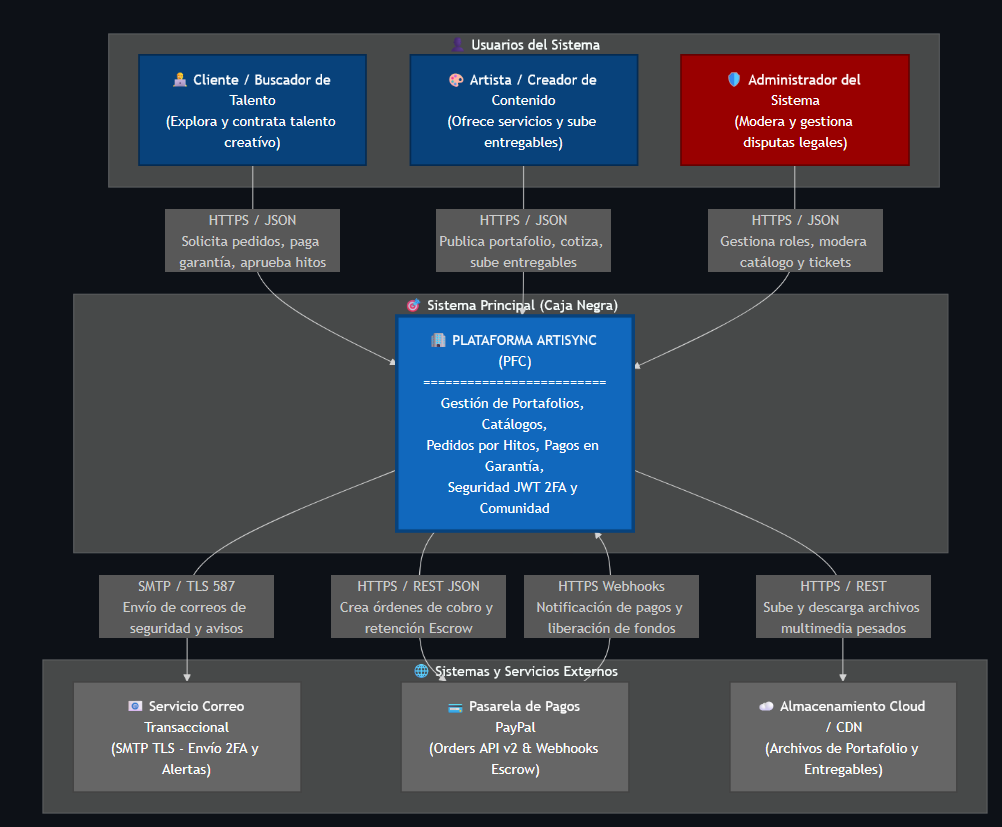
\includegraphics[width=6.29407in,height=5.19444in]{media/media/image1.png}\emph{Figura
1. Diagrama C4 Nivel 1 --- Diagrama de contexto del Software Artisync.}

\subsubsection{\texorpdfstring{\textbf{Descripción formal del sistema y
sus interacciones
externas}}{Descripción formal del sistema y sus interacciones externas}}\label{descripciuxf3n-formal-del-sistema-y-sus-interacciones-externas}

Artisync es una plataforma web de gestión de comisiones de contenido
digital que actúa como nodo central entre tres perfiles de usuario y
tres servicios externos. El diagrama representa el sistema como una
unidad indivisible, definiendo sus límites y los flujos de información
que cruzan esa frontera sin exponer su estructura interna,
correspondiendo al Nivel 1 del modelo C4.

El Creador envía datos de perfil, servicios, documentos para
verificación y entregables firmados electrónicamente. Recibe
notificaciones de estado, confirmaciones de garantía, mensajes en tiempo
real y alertas de infracción. El Cliente envía solicitudes de
contratación, respuestas al briefing, firma del contrato y aprobación
del entregable. Recibe el catálogo de servicios, contratos en PDF,
mensajes en tiempo real y la descarga del entregable limpio tras liberar
el pago. El Administrador envía configuraciones globales, el umbral de
confianza de la IA y resoluciones de disputas. Recibe reportes contables
en CSV, alertas de comportamiento y registros de auditoría completos.

La API de PayPal Orders v2 es el único canal financiero de la
plataforma: recibe las órdenes de pago generadas por Artisync y devuelve
confirmaciones mediante webhooks firmados que el sistema verifica antes
de liberar fondos. El Servicio de Inteligencia Artificial recibe
documentos de identidad y certificados profesionales, y devuelve el
resultado de verificación de mayoría de edad y un puntaje de confianza
decimal que determina la asignación del sello de verificación en el
perfil del Creador. El Servicio de Almacenamiento S3 recibe todos los
archivos binarios de la plataforma y devuelve las URLs públicas que la
interfaz utiliza para renderizar contenido y habilitar descargas,
manteniendo al servidor de aplicaciones libre de gestión de archivos
locales.

\subsubsection{\texorpdfstring{\textbf{Diagrama C4 Nivel 2: Contenedores
de Software}
}{Diagrama C4 Nivel 2: Contenedores de Software }}\label{diagrama-c4-nivel-2-contenedores-de-software}

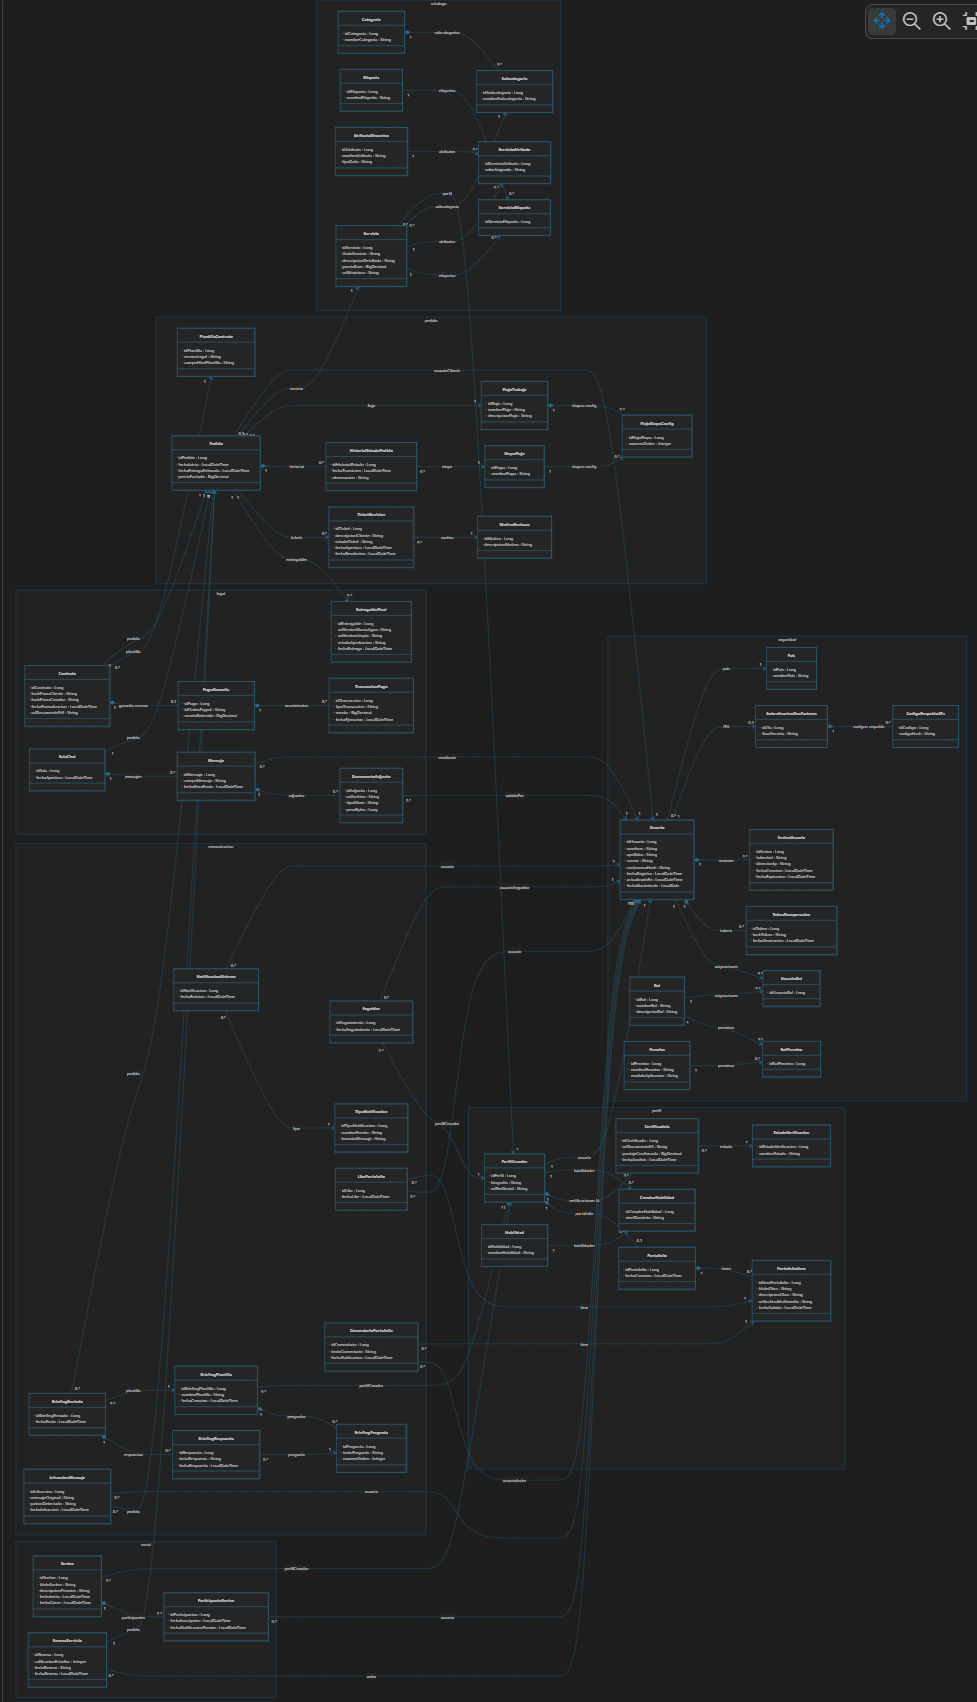
\includegraphics[width=5.19444in,height=7.20984in]{media/media/image2.png}

\emph{Figura 2. Diagrama C4 Nivel 2 --- Contenedores de Software
Artisync.}

El diagrama de contenedores desglosa el sistema en sus piezas de
software principales, mostrando cómo los usuarios (User) y
administradores (Admin) acceden e interactúan directamente con la
Aplicación Web (Frontend) basada en Angular y TypeScript. Este
contenedor de frontend se ejecuta en el navegador del usuario y se
comunica de forma asíncrona mediante `HTTP/JSON` con el Servidor de
Aplicaciones (Backend) desarrollado en Spring Boot, el cual centraliza
la lógica de negocio (Business Logic), gestiona la seguridad y expone
una API REST. A su vez, este backend se conecta mediante `JDBC` a la
base de datos PostgreSQL para la persistencia transaccional, al mismo
tiempo que realiza peticiones salientes vía `REST API` hacia tres
servicios externos esenciales: la API de PayPal para procesar flujos de
pago y depósitos en garantía (Pay Escrow), AWS S3 o Cloudflare R2 para
el almacenamiento seguro de archivos (Store Files), y un Motor de IA
dedicado a la automatización de la verificación de certificados.

\begin{quote}
\textbf{4.2. Descripción de capas y tecnologías}
\end{quote}

\begin{longtable}[]{@{}
  >{\raggedright\arraybackslash}p{(\columnwidth - 4\tabcolsep) * \real{0.1881}}
  >{\raggedright\arraybackslash}p{(\columnwidth - 4\tabcolsep) * \real{0.2359}}
  >{\raggedright\arraybackslash}p{(\columnwidth - 4\tabcolsep) * \real{0.5760}}@{}}
\toprule\noalign{}
\begin{minipage}[b]{\linewidth}\raggedright
\textbf{Capa}
\end{minipage} & \begin{minipage}[b]{\linewidth}\raggedright
\textbf{Tecnología elegida}
\end{minipage} & \begin{minipage}[b]{\linewidth}\raggedright
\textbf{Justificación}
\end{minipage} \\
\midrule\noalign{}
\endhead
\bottomrule\noalign{}
\endlastfoot
Frontend & Angular 19, TypeScript, CSS3, Bootstrap 5 & Angular
proporciona un framework con inyección de dependencias, módulos
lazy-loading y compilación AOT que optimizan el rendimiento. TypeScript
añade tipado estático, reduciendo errores en tiempo de desarrollo.
Bootstrap 5 + CSS3 permite construir interfaces responsivas con clases
utilitarias sin añadir CSS muerto al bundle de producción. \\
Framework CSS & Bootstrap 5, CSS3 & Bootstrap 5 fue elegido por su
sistema de grilla de 12 columnas, componentes responsivos nativos
(modales, formularios, navbar) y su amplia documentación. Combinado con
CSS3 personalizado permite construir la identidad visual de Artisync sin
abandonar estándares web. La curva de aprendizaje es baja y el equipo ya
tiene experiencia previa con el framework. \\
Backend & Java 25 con Spring Boot 4.0.6 & Java 25 ofrece soporte a largo
plazo (LTS) y virtual threads (Project Loom) para alta concurrencia.
Spring Boot 4.0.6 reduce la configuración boilerplate y cuenta con el
ecosistema más maduro para aplicaciones empresariales: Spring Security,
Spring Data JPA y Spring Batch, todos coherentes con los módulos de la
base de datos Artisync. \\
Framework backend & Spring Boot 4.0.6, Spring Security, JPA & Spring
Security gestiona el control de acceso basado en roles (RBAC).
JPA/Hibernate mapea automáticamente las entidades del esquema
relacional. Spring Boot Actuator facilita el monitoreo del sistema en
producción. \\
Base de datos & PostgreSQL 18 & PostgreSQL 18 soporta transacciones
ACID, constraints complejos (ENUM via CHECK, UNIQUE compuestos) y tipos
de datos avanzados (DECIMAL(10,2) para montos financieros, TEXT para
contratos HTML). Su robustez garantiza la integridad del patrón Escrow
implementado en pagos\_garantia y transacciones\_pago. \\
Control de versiones & Git, GitHub & Repositorio compartido del equipo
con estrategia de ramas (main, develop, feature/*). \\
Despliegue & Docker, Docker Compose & Docker permite empaquetar cada
contenedor (Angular build, Spring Boot JAR, PostgreSQL) con sus
dependencias aisladas. Docker Compose orquesta el arranque en orden
correcto y define las redes internas. Esto garantiza paridad total entre
el entorno de desarrollo local y el servidor de producción. \\
\end{longtable}

\begin{quote}
\textbf{4.3. ADR-001: Decisión de tecnología principal}
\end{quote}

El siguiente Architecture Decision Record (ADR) documenta de forma
formal y trazable la decisión más crítica del proyecto: la elección del
lenguaje y framework del servidor.

\begin{longtable}[]{@{}
  >{\raggedright\arraybackslash}p{(\columnwidth - 2\tabcolsep) * \real{0.1853}}
  >{\raggedright\arraybackslash}p{(\columnwidth - 2\tabcolsep) * \real{0.8147}}@{}}
\toprule\noalign{}
\begin{minipage}[b]{\linewidth}\raggedright
\textbf{Título}
\end{minipage} & \begin{minipage}[b]{\linewidth}\raggedright
ADR-001: Selección del lenguaje de programación del servidor
\end{minipage} \\
\midrule\noalign{}
\endhead
\bottomrule\noalign{}
\endlastfoot
\textbf{Estado} & En Revisión \\
\textbf{Fecha} & Semana 5 --- Período académico 2025-2026 \\
\textbf{Contexto} & El equipo de desarrollo de Artisync debe seleccionar
el lenguaje y entorno del lado del servidor para implementar la lógica
de negocio del sistema. Las restricciones que enmarcan esta decisión son
las siguientes:

1. Tiempo disponible: 14 semanas de desarrollo divididas en entregas
parciales.

2. Conocimiento previo: el equipo tiene experiencia con Java (cursos de
POO y Estructuras de Datos) y ha trabajado con Spring Boot en prácticas
de laboratorio y proyectos personales.

3. Requisitos del sistema: el backend debe implementar RBAC (tablas
roles/permisos), JWT con 2FA, el patrón Escrow financiero y un motor de
flujos de trabajo parametrizable.

4. Hosting disponible: por el momento localmente.

5. Madurez del ecosistema: se requieren librerías estables para
integración con PayPal, AWS S3 / Cloudflare R2 y servicios SMTP. \\
\textbf{Opciones consideradas} & Opción A --- Spring Boot (Java 25):
Plataforma basada en Java diseñada para crear aplicaciones robustas,
escalables y listas para producción. Destaca por tener la mejor
velocidad de procesamiento de peticiones y una alta fiabilidad en cargas
de hasta 8,000 usuarios simultáneos. Incluye mecanismos de optimización
de rendimiento integrados por defecto.

Opción B --- Express (JavaScript/Node.js 4.18.2): Ecosistema diseñado
para optimizar la eficiencia y escalabilidad mediante un enfoque
minimalista. Aunque es más lento que Spring Boot en el procesamiento,
demuestra una mayor fiabilidad (menor tasa de errores) bajo cargas
extremas de 16,000 usuarios simultáneos. Requiere bibliotecas
adicionales y configuración manual para implementar mecanismos de alto
rendimiento.

Opción C --- Django (Python 3.11): Framework de alto nivel que permite
el desarrollo rápido, pero registra la eficiencia más baja en pruebas
comparativas. Presenta los tiempos de procesamiento más largos y la
mayor tasa de errores debido a su arquitectura basada en hilos, lo que
eleva el consumo de memoria y procesamiento bajo carga sustancial \\
\textbf{Decisión} & Se elige la Opción A: Java 25 con Spring Boot 4.0.6.

Spring Boot 4.0.6 proporciona, fuera de la caja, los módulos exactos que
Artisync requiere: Spring Security para RBAC y JWT, Spring Data
JPA/Hibernate para el mapeo del esquema relacional de 42 tablas, y
Spring Boot Actuator para observabilidad. La curva de aprendizaje
adicional se mitiga con la experiencia previa del equipo en Java y la
documentación oficial extensa. Adicionalmente, Java 25 introduce virtual
threads (Project Loom) que mejoran la escalabilidad del sistema de
mensajería en tiempo real (módulo salas\_chat y mensajes) sin cambiar el
modelo de programación. \\
\textbf{Consecuencias positivas} & • Control de acceso (RBAC)
implementado con Spring Security y las tablas roles/permisos sin código
adicional de seguridad manual.

• JPA/Hibernate genera el DDL automáticamente desde las entidades,
reduciendo errores de sincronización con el esquema PostgreSQL.

• SDKs oficiales de AWS S3 / Cloudflare R2 (SDK Java) y PayPal para
Java, garantizando soporte a largo plazo.

• Java 25 LTS: soporte de seguridad garantizado hasta 2033.

• Ecosistema maduro que simplifica la configuración y el despliegue de
aplicaciones mediante la inyección de dependencias y el uso de
anotaciones \\
\textbf{Consecuencias negativas} & • Mayor complejidad inicial en
comparación con frameworks minimalistas, requiriendo un conocimiento más
profundo de sus mecanismos integrados para su aprovechamiento óptimo

• Verbosidad del lenguaje: mitigada con Lombok para reducir boilerplate
(getters, setters, constructores).

• Curva de aprendizaje de Spring Security: mitigada con módulos
incrementales y revisión de código en equipo. \\
\end{longtable}

\textbf{5. Modelo de base de datos}

\begin{quote}
\textbf{5.1. Modelo Entidad-Relación (MER)}
\end{quote}

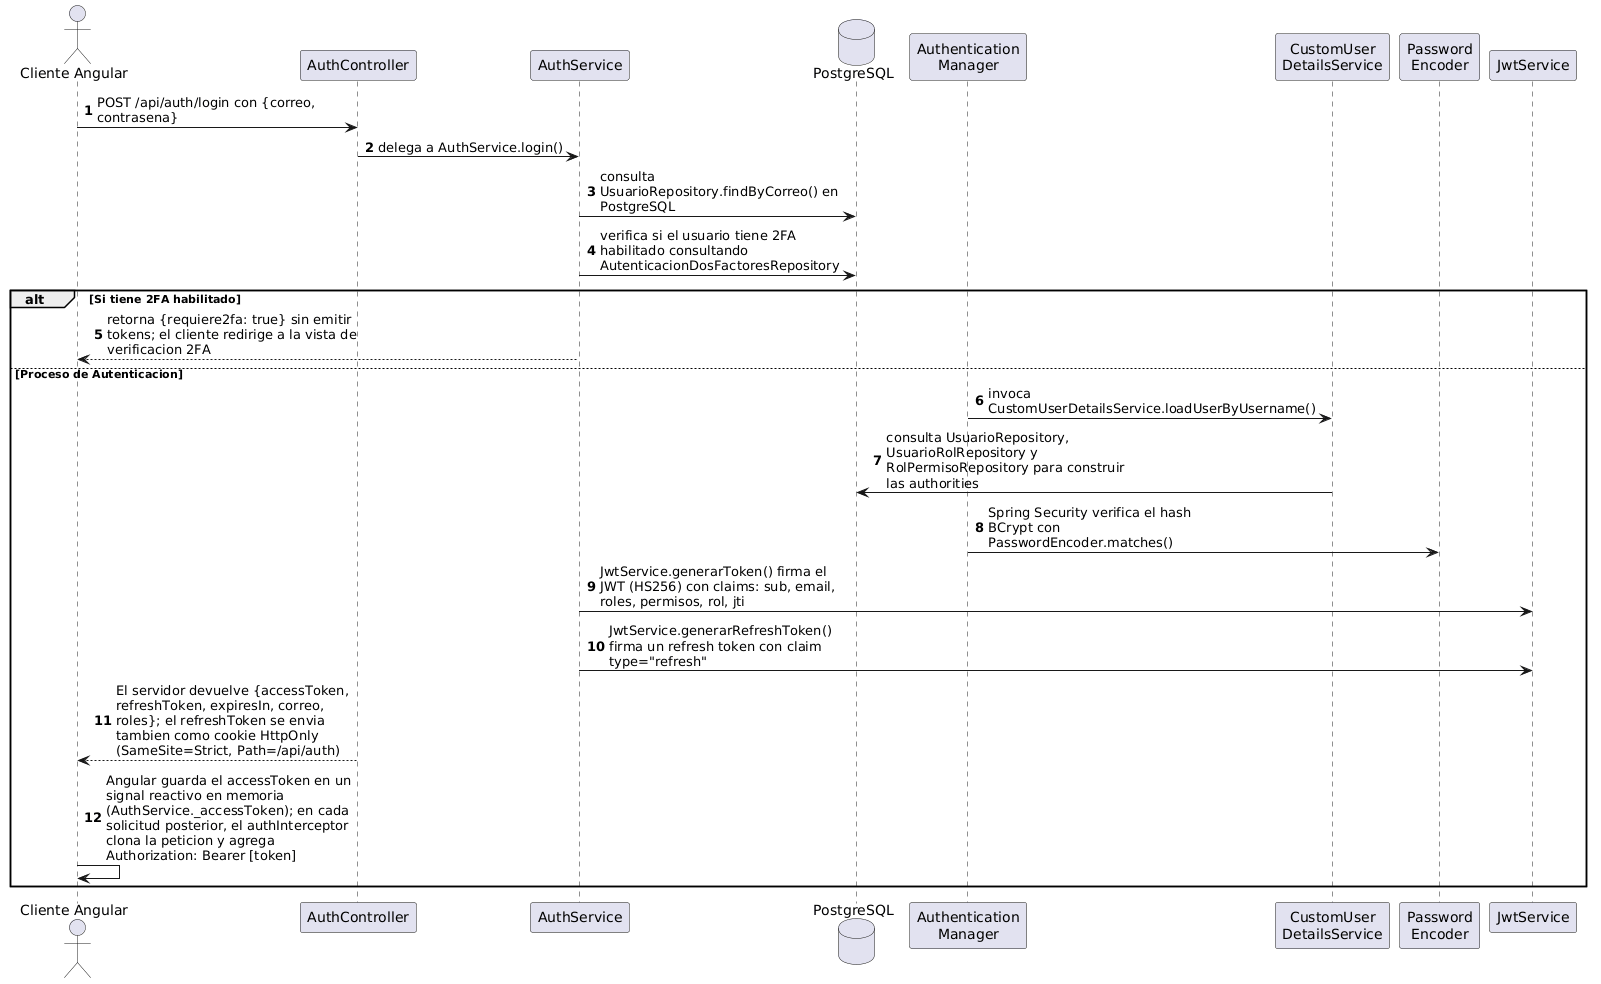
\includegraphics[width=6.22046in,height=5.2156in]{media/media/image3.png}\emph{Figura
3. Diagrama de base de datos de Artisync.}

\begin{quote}
\textbf{5.2. Diccionario de datos}
\end{quote}

Módulo 1: Seguridad y Control de Acceso

Tabla: roles

\begin{longtable}[]{@{}
  >{\raggedright\arraybackslash}p{(\columnwidth - 8\tabcolsep) * \real{0.2000}}
  >{\raggedright\arraybackslash}p{(\columnwidth - 8\tabcolsep) * \real{0.2000}}
  >{\raggedright\arraybackslash}p{(\columnwidth - 8\tabcolsep) * \real{0.2000}}
  >{\raggedright\arraybackslash}p{(\columnwidth - 8\tabcolsep) * \real{0.2000}}
  >{\raggedright\arraybackslash}p{(\columnwidth - 8\tabcolsep) * \real{0.2000}}@{}}
\toprule\noalign{}
\begin{minipage}[b]{\linewidth}\raggedright
\textbf{Atributo}
\end{minipage} & \begin{minipage}[b]{\linewidth}\raggedright
\textbf{Tipo}
\end{minipage} & \begin{minipage}[b]{\linewidth}\raggedright
\textbf{Nulo}
\end{minipage} & \begin{minipage}[b]{\linewidth}\raggedright
\textbf{Restricción}
\end{minipage} & \begin{minipage}[b]{\linewidth}\raggedright
\textbf{Descripción}
\end{minipage} \\
\midrule\noalign{}
\endhead
\bottomrule\noalign{}
\endlastfoot
id\_rol & SERIAL & No & PK, AUTO & Identificador único del rol \\
nombre\_rol & VARCHAR(50) & No & NOT NULL, UNIQUE & Nombre único del
rol \\
descripcion\_rol & TEXT & Sí & & Descripción del rol \\
\end{longtable}

Tabla: permisos

\begin{longtable}[]{@{}
  >{\raggedright\arraybackslash}p{(\columnwidth - 8\tabcolsep) * \real{0.2000}}
  >{\raggedright\arraybackslash}p{(\columnwidth - 8\tabcolsep) * \real{0.2000}}
  >{\raggedright\arraybackslash}p{(\columnwidth - 8\tabcolsep) * \real{0.2000}}
  >{\raggedright\arraybackslash}p{(\columnwidth - 8\tabcolsep) * \real{0.2000}}
  >{\raggedright\arraybackslash}p{(\columnwidth - 8\tabcolsep) * \real{0.2001}}@{}}
\toprule\noalign{}
\begin{minipage}[b]{\linewidth}\raggedright
\textbf{Atributo}
\end{minipage} & \begin{minipage}[b]{\linewidth}\raggedright
\textbf{Tipo}
\end{minipage} & \begin{minipage}[b]{\linewidth}\raggedright
\textbf{Nulo}
\end{minipage} & \begin{minipage}[b]{\linewidth}\raggedright
\textbf{Restricción}
\end{minipage} & \begin{minipage}[b]{\linewidth}\raggedright
\textbf{Descripción}
\end{minipage} \\
\midrule\noalign{}
\endhead
\bottomrule\noalign{}
\endlastfoot
id\_permiso & SERIAL & No & PK, AUTO & Identificador único del
permiso \\
nombre\_permiso & VARCHAR(100) & No & NOT NULL, UNIQUE & Nombre único
del permiso \\
modulo\_aplicacion & VARCHAR(50) & Sí & & Módulo al que pertenece el
permiso \\
\end{longtable}

Tabla: rol\_permisos

\begin{longtable}[]{@{}
  >{\raggedright\arraybackslash}p{(\columnwidth - 8\tabcolsep) * \real{0.2000}}
  >{\raggedright\arraybackslash}p{(\columnwidth - 8\tabcolsep) * \real{0.2000}}
  >{\raggedright\arraybackslash}p{(\columnwidth - 8\tabcolsep) * \real{0.2000}}
  >{\raggedright\arraybackslash}p{(\columnwidth - 8\tabcolsep) * \real{0.2000}}
  >{\raggedright\arraybackslash}p{(\columnwidth - 8\tabcolsep) * \real{0.2000}}@{}}
\toprule\noalign{}
\begin{minipage}[b]{\linewidth}\raggedright
\textbf{Atributo}
\end{minipage} & \begin{minipage}[b]{\linewidth}\raggedright
\textbf{Tipo}
\end{minipage} & \begin{minipage}[b]{\linewidth}\raggedright
\textbf{Nulo}
\end{minipage} & \begin{minipage}[b]{\linewidth}\raggedright
\textbf{Restricción}
\end{minipage} & \begin{minipage}[b]{\linewidth}\raggedright
\textbf{Descripción}
\end{minipage} \\
\midrule\noalign{}
\endhead
\bottomrule\noalign{}
\endlastfoot
id\_rol\_permiso & SERIAL & No & PK, AUTO & Identificador único de la
relación \\
id\_rol & INT & No & FK → roles & Referencia al rol \\
id\_permiso & INT & No & FK → permisos & Referencia al permiso \\
\end{longtable}

Tabla: pais

\begin{longtable}[]{@{}
  >{\raggedright\arraybackslash}p{(\columnwidth - 8\tabcolsep) * \real{0.2000}}
  >{\raggedright\arraybackslash}p{(\columnwidth - 8\tabcolsep) * \real{0.2000}}
  >{\raggedright\arraybackslash}p{(\columnwidth - 8\tabcolsep) * \real{0.2000}}
  >{\raggedright\arraybackslash}p{(\columnwidth - 8\tabcolsep) * \real{0.2000}}
  >{\raggedright\arraybackslash}p{(\columnwidth - 8\tabcolsep) * \real{0.2000}}@{}}
\toprule\noalign{}
\begin{minipage}[b]{\linewidth}\raggedright
\textbf{Atributo}
\end{minipage} & \begin{minipage}[b]{\linewidth}\raggedright
\textbf{Tipo}
\end{minipage} & \begin{minipage}[b]{\linewidth}\raggedright
\textbf{Nulo}
\end{minipage} & \begin{minipage}[b]{\linewidth}\raggedright
\textbf{Restricción}
\end{minipage} & \begin{minipage}[b]{\linewidth}\raggedright
\textbf{Descripción}
\end{minipage} \\
\midrule\noalign{}
\endhead
\bottomrule\noalign{}
\endlastfoot
id\_pais & SERIAL & No & PK, AUTO & Identificador único del país \\
nombre\_pais & VARCHAR(100) & No & NOT NULL, UNIQUE & Nombre del país \\
\end{longtable}

Tabla: usuarios

\begin{longtable}[]{@{}
  >{\raggedright\arraybackslash}p{(\columnwidth - 8\tabcolsep) * \real{0.2000}}
  >{\raggedright\arraybackslash}p{(\columnwidth - 8\tabcolsep) * \real{0.2000}}
  >{\raggedright\arraybackslash}p{(\columnwidth - 8\tabcolsep) * \real{0.2000}}
  >{\raggedright\arraybackslash}p{(\columnwidth - 8\tabcolsep) * \real{0.2000}}
  >{\raggedright\arraybackslash}p{(\columnwidth - 8\tabcolsep) * \real{0.2000}}@{}}
\toprule\noalign{}
\begin{minipage}[b]{\linewidth}\raggedright
\textbf{Atributo}
\end{minipage} & \begin{minipage}[b]{\linewidth}\raggedright
\textbf{Tipo}
\end{minipage} & \begin{minipage}[b]{\linewidth}\raggedright
\textbf{Nulo}
\end{minipage} & \begin{minipage}[b]{\linewidth}\raggedright
\textbf{Restricción}
\end{minipage} & \begin{minipage}[b]{\linewidth}\raggedright
\textbf{Descripción}
\end{minipage} \\
\midrule\noalign{}
\endhead
\bottomrule\noalign{}
\endlastfoot
id\_usuario & SERIAL & No & PK, AUTO & Identificador único del
usuario \\
nombres & VARCHAR(100) & No & NOT NULL & Nombres del usuario \\
apellidos & VARCHAR(100) & No & NOT NULL & Apellidos del usuario \\
correo & VARCHAR(150) & No & NOT NULL, UNIQUE & Correo electrónico
(usado para login) \\
contrasena\_hash & VARCHAR(255) & No & NOT NULL & Hash de la
contraseña \\
id\_pais & INT & Sí & FK → pais & País del usuario \\
fecha\_registro & TIMESTAMP & No & DEFAULT NOW() & Fecha y hora de
registro \\
estado\_cuenta & BOOLEAN & No & DEFAULT TRUE & Estado activo/inactivo de
la cuenta \\
\end{longtable}

Tabla: usuario\_roles

\begin{longtable}[]{@{}
  >{\raggedright\arraybackslash}p{(\columnwidth - 8\tabcolsep) * \real{0.2000}}
  >{\raggedright\arraybackslash}p{(\columnwidth - 8\tabcolsep) * \real{0.2000}}
  >{\raggedright\arraybackslash}p{(\columnwidth - 8\tabcolsep) * \real{0.2000}}
  >{\raggedright\arraybackslash}p{(\columnwidth - 8\tabcolsep) * \real{0.2000}}
  >{\raggedright\arraybackslash}p{(\columnwidth - 8\tabcolsep) * \real{0.2000}}@{}}
\toprule\noalign{}
\begin{minipage}[b]{\linewidth}\raggedright
\textbf{Atributo}
\end{minipage} & \begin{minipage}[b]{\linewidth}\raggedright
\textbf{Tipo}
\end{minipage} & \begin{minipage}[b]{\linewidth}\raggedright
\textbf{Nulo}
\end{minipage} & \begin{minipage}[b]{\linewidth}\raggedright
\textbf{Restricción}
\end{minipage} & \begin{minipage}[b]{\linewidth}\raggedright
\textbf{Descripción}
\end{minipage} \\
\midrule\noalign{}
\endhead
\bottomrule\noalign{}
\endlastfoot
id\_usuario\_rol & SERIAL & No & PK, AUTO & Identificador único de la
relación \\
id\_usuario & INT & No & FK → usuarios & Referencia al usuario \\
id\_rol & INT & No & FK → roles & Referencia al rol \\
\end{longtable}

Tabla: sesiones\_usuario

\begin{longtable}[]{@{}
  >{\raggedright\arraybackslash}p{(\columnwidth - 8\tabcolsep) * \real{0.2000}}
  >{\raggedright\arraybackslash}p{(\columnwidth - 8\tabcolsep) * \real{0.2000}}
  >{\raggedright\arraybackslash}p{(\columnwidth - 8\tabcolsep) * \real{0.2000}}
  >{\raggedright\arraybackslash}p{(\columnwidth - 8\tabcolsep) * \real{0.2000}}
  >{\raggedright\arraybackslash}p{(\columnwidth - 8\tabcolsep) * \real{0.2000}}@{}}
\toprule\noalign{}
\begin{minipage}[b]{\linewidth}\raggedright
\textbf{Atributo}
\end{minipage} & \begin{minipage}[b]{\linewidth}\raggedright
\textbf{Tipo}
\end{minipage} & \begin{minipage}[b]{\linewidth}\raggedright
\textbf{Nulo}
\end{minipage} & \begin{minipage}[b]{\linewidth}\raggedright
\textbf{Restricción}
\end{minipage} & \begin{minipage}[b]{\linewidth}\raggedright
\textbf{Descripción}
\end{minipage} \\
\midrule\noalign{}
\endhead
\bottomrule\noalign{}
\endlastfoot
id\_sesion & SERIAL & No & PK, AUTO & Identificador único de la
sesión \\
id\_usuario & INT & No & FK → usuarios & Referencia al usuario \\
token\_jwt & TEXT & No & NOT NULL & Token JWT de la sesión \\
direccion\_ip & VARCHAR(45) & Sí & & Dirección IP del cliente \\
fecha\_creacion & TIMESTAMP & No & DEFAULT NOW() & Fecha de creación de
la sesión \\
fecha\_expiracion & TIMESTAMP & No & NOT NULL & Fecha de expiración del
token \\
\end{longtable}

Tabla: tokens\_recuperacion

\begin{longtable}[]{@{}
  >{\raggedright\arraybackslash}p{(\columnwidth - 8\tabcolsep) * \real{0.2000}}
  >{\raggedright\arraybackslash}p{(\columnwidth - 8\tabcolsep) * \real{0.2000}}
  >{\raggedright\arraybackslash}p{(\columnwidth - 8\tabcolsep) * \real{0.2000}}
  >{\raggedright\arraybackslash}p{(\columnwidth - 8\tabcolsep) * \real{0.2000}}
  >{\raggedright\arraybackslash}p{(\columnwidth - 8\tabcolsep) * \real{0.2000}}@{}}
\toprule\noalign{}
\begin{minipage}[b]{\linewidth}\raggedright
\textbf{Atributo}
\end{minipage} & \begin{minipage}[b]{\linewidth}\raggedright
\textbf{Tipo}
\end{minipage} & \begin{minipage}[b]{\linewidth}\raggedright
\textbf{Nulo}
\end{minipage} & \begin{minipage}[b]{\linewidth}\raggedright
\textbf{Restricción}
\end{minipage} & \begin{minipage}[b]{\linewidth}\raggedright
\textbf{Descripción}
\end{minipage} \\
\midrule\noalign{}
\endhead
\bottomrule\noalign{}
\endlastfoot
id\_token & SERIAL & No & PK, AUTO & Identificador único del token \\
id\_usuario & INT & No & FK → usuarios & Referencia al usuario \\
hash\_token & VARCHAR(255) & No & NOT NULL & Hash del token de
recuperación \\
fecha\_generacion & TIMESTAMP & No & DEFAULT NOW() & Fecha de generación
del token \\
usado & BOOLEAN & No & DEFAULT FALSE & Indica si el token ya fue
usado \\
\end{longtable}

Tabla: autenticacion\_dos\_factores

\begin{longtable}[]{@{}
  >{\raggedright\arraybackslash}p{(\columnwidth - 8\tabcolsep) * \real{0.2000}}
  >{\raggedright\arraybackslash}p{(\columnwidth - 8\tabcolsep) * \real{0.2000}}
  >{\raggedright\arraybackslash}p{(\columnwidth - 8\tabcolsep) * \real{0.2000}}
  >{\raggedright\arraybackslash}p{(\columnwidth - 8\tabcolsep) * \real{0.2000}}
  >{\raggedright\arraybackslash}p{(\columnwidth - 8\tabcolsep) * \real{0.2000}}@{}}
\toprule\noalign{}
\begin{minipage}[b]{\linewidth}\raggedright
\textbf{Atributo}
\end{minipage} & \begin{minipage}[b]{\linewidth}\raggedright
\textbf{Tipo}
\end{minipage} & \begin{minipage}[b]{\linewidth}\raggedright
\textbf{Nulo}
\end{minipage} & \begin{minipage}[b]{\linewidth}\raggedright
\textbf{Restricción}
\end{minipage} & \begin{minipage}[b]{\linewidth}\raggedright
\textbf{Descripción}
\end{minipage} \\
\midrule\noalign{}
\endhead
\bottomrule\noalign{}
\endlastfoot
id\_2fa & SERIAL & No & PK, AUTO & Identificador único del registro
2FA \\
id\_usuario & INT & No & FK → usuarios, UNIQUE & Referencia al usuario
(uno a uno) \\
llave\_secreta & VARCHAR(255) & No & NOT NULL & Llave secreta para
2FA \\
esta\_habilitado & BOOLEAN & No & DEFAULT FALSE & Indica si el 2FA está
activo \\
\end{longtable}

Módulo 2: Perfiles, Verificación y Portafolio

Tabla: perfiles\_creadores

\begin{longtable}[]{@{}
  >{\raggedright\arraybackslash}p{(\columnwidth - 8\tabcolsep) * \real{0.2000}}
  >{\raggedright\arraybackslash}p{(\columnwidth - 8\tabcolsep) * \real{0.2000}}
  >{\raggedright\arraybackslash}p{(\columnwidth - 8\tabcolsep) * \real{0.2000}}
  >{\raggedright\arraybackslash}p{(\columnwidth - 8\tabcolsep) * \real{0.2000}}
  >{\raggedright\arraybackslash}p{(\columnwidth - 8\tabcolsep) * \real{0.2000}}@{}}
\toprule\noalign{}
\begin{minipage}[b]{\linewidth}\raggedright
\textbf{Atributo}
\end{minipage} & \begin{minipage}[b]{\linewidth}\raggedright
\textbf{Tipo}
\end{minipage} & \begin{minipage}[b]{\linewidth}\raggedright
\textbf{Nulo}
\end{minipage} & \begin{minipage}[b]{\linewidth}\raggedright
\textbf{Restricción}
\end{minipage} & \begin{minipage}[b]{\linewidth}\raggedright
\textbf{Descripción}
\end{minipage} \\
\midrule\noalign{}
\endhead
\bottomrule\noalign{}
\endlastfoot
id\_perfil & SERIAL & No & PK, AUTO & Identificador único del perfil \\
id\_usuario & INT & No & FK → usuarios, UNIQUE & Referencia al usuario
(uno a uno) \\
biografia & TEXT & Sí & & Biografía del creador \\
url\_red\_social & VARCHAR(255) & Sí & & URL de red social del
creador \\
\end{longtable}

Tabla: estados\_verificacion

\begin{longtable}[]{@{}
  >{\raggedright\arraybackslash}p{(\columnwidth - 8\tabcolsep) * \real{0.2000}}
  >{\raggedright\arraybackslash}p{(\columnwidth - 8\tabcolsep) * \real{0.2000}}
  >{\raggedright\arraybackslash}p{(\columnwidth - 8\tabcolsep) * \real{0.2000}}
  >{\raggedright\arraybackslash}p{(\columnwidth - 8\tabcolsep) * \real{0.2000}}
  >{\raggedright\arraybackslash}p{(\columnwidth - 8\tabcolsep) * \real{0.2001}}@{}}
\toprule\noalign{}
\begin{minipage}[b]{\linewidth}\raggedright
\textbf{Atributo}
\end{minipage} & \begin{minipage}[b]{\linewidth}\raggedright
\textbf{Tipo}
\end{minipage} & \begin{minipage}[b]{\linewidth}\raggedright
\textbf{Nulo}
\end{minipage} & \begin{minipage}[b]{\linewidth}\raggedright
\textbf{Restricción}
\end{minipage} & \begin{minipage}[b]{\linewidth}\raggedright
\textbf{Descripción}
\end{minipage} \\
\midrule\noalign{}
\endhead
\bottomrule\noalign{}
\endlastfoot
id\_estado\_verificacion & SERIAL & No & PK, AUTO & Identificador único
del estado \\
nombre\_estado & VARCHAR(50) & No & NOT NULL, UNIQUE & Nombre del estado
(ej: Pendiente, Aprobado) \\
\end{longtable}

Tabla: certificados\_ia

\begin{longtable}[]{@{}
  >{\raggedright\arraybackslash}p{(\columnwidth - 8\tabcolsep) * \real{0.2000}}
  >{\raggedright\arraybackslash}p{(\columnwidth - 8\tabcolsep) * \real{0.2000}}
  >{\raggedright\arraybackslash}p{(\columnwidth - 8\tabcolsep) * \real{0.2000}}
  >{\raggedright\arraybackslash}p{(\columnwidth - 8\tabcolsep) * \real{0.2000}}
  >{\raggedright\arraybackslash}p{(\columnwidth - 8\tabcolsep) * \real{0.2001}}@{}}
\toprule\noalign{}
\begin{minipage}[b]{\linewidth}\raggedright
\textbf{Atributo}
\end{minipage} & \begin{minipage}[b]{\linewidth}\raggedright
\textbf{Tipo}
\end{minipage} & \begin{minipage}[b]{\linewidth}\raggedright
\textbf{Nulo}
\end{minipage} & \begin{minipage}[b]{\linewidth}\raggedright
\textbf{Restricción}
\end{minipage} & \begin{minipage}[b]{\linewidth}\raggedright
\textbf{Descripción}
\end{minipage} \\
\midrule\noalign{}
\endhead
\bottomrule\noalign{}
\endlastfoot
id\_certificado & SERIAL & No & PK, AUTO & Identificador único del
certificado \\
id\_perfil & INT & No & FK → perfiles\_creadores & Referencia al perfil
del creador \\
id\_estado\_verificacion & INT & No & FK → estados\_verificacion &
Estado actual del certificado \\
url\_documento\_s3 & VARCHAR(255) & No & NOT NULL & URL del documento en
S3 \\
puntaje\_confianza\_ia & DECIMAL(5,2) & Sí & & Puntaje de confianza
asignado por IA \\
fecha\_analisis & TIMESTAMP & No & DEFAULT NOW() & Fecha del análisis
del certificado \\
\end{longtable}

Tabla: habilidades

\begin{longtable}[]{@{}
  >{\raggedright\arraybackslash}p{(\columnwidth - 8\tabcolsep) * \real{0.2000}}
  >{\raggedright\arraybackslash}p{(\columnwidth - 8\tabcolsep) * \real{0.2000}}
  >{\raggedright\arraybackslash}p{(\columnwidth - 8\tabcolsep) * \real{0.2000}}
  >{\raggedright\arraybackslash}p{(\columnwidth - 8\tabcolsep) * \real{0.2000}}
  >{\raggedright\arraybackslash}p{(\columnwidth - 8\tabcolsep) * \real{0.2001}}@{}}
\toprule\noalign{}
\begin{minipage}[b]{\linewidth}\raggedright
\textbf{Atributo}
\end{minipage} & \begin{minipage}[b]{\linewidth}\raggedright
\textbf{Tipo}
\end{minipage} & \begin{minipage}[b]{\linewidth}\raggedright
\textbf{Nulo}
\end{minipage} & \begin{minipage}[b]{\linewidth}\raggedright
\textbf{Restricción}
\end{minipage} & \begin{minipage}[b]{\linewidth}\raggedright
\textbf{Descripción}
\end{minipage} \\
\midrule\noalign{}
\endhead
\bottomrule\noalign{}
\endlastfoot
id\_habilidad & SERIAL & No & PK, AUTO & Identificador único de la
habilidad \\
nombre\_habilidad & VARCHAR(100) & No & NOT NULL, UNIQUE & Nombre de la
habilidad \\
\end{longtable}

Tabla: creador\_habilidades

\begin{longtable}[]{@{}
  >{\raggedright\arraybackslash}p{(\columnwidth - 8\tabcolsep) * \real{0.2000}}
  >{\raggedright\arraybackslash}p{(\columnwidth - 8\tabcolsep) * \real{0.2000}}
  >{\raggedright\arraybackslash}p{(\columnwidth - 8\tabcolsep) * \real{0.2000}}
  >{\raggedright\arraybackslash}p{(\columnwidth - 8\tabcolsep) * \real{0.2000}}
  >{\raggedright\arraybackslash}p{(\columnwidth - 8\tabcolsep) * \real{0.2001}}@{}}
\toprule\noalign{}
\begin{minipage}[b]{\linewidth}\raggedright
\textbf{Atributo}
\end{minipage} & \begin{minipage}[b]{\linewidth}\raggedright
\textbf{Tipo}
\end{minipage} & \begin{minipage}[b]{\linewidth}\raggedright
\textbf{Nulo}
\end{minipage} & \begin{minipage}[b]{\linewidth}\raggedright
\textbf{Restricción}
\end{minipage} & \begin{minipage}[b]{\linewidth}\raggedright
\textbf{Descripción}
\end{minipage} \\
\midrule\noalign{}
\endhead
\bottomrule\noalign{}
\endlastfoot
id\_creador\_habilidad & SERIAL & No & PK, AUTO & Identificador único de
la relación \\
id\_perfil & INT & No & FK → perfiles\_creadores & Referencia al perfil
del creador \\
id\_habilidad & INT & No & FK → habilidades & Referencia a la
habilidad \\
nivel\_dominio & VARCHAR(50) & Sí & & Nivel: Básico, Intermedio,
Experto \\
\end{longtable}

Tabla: portafolios

\begin{longtable}[]{@{}
  >{\raggedright\arraybackslash}p{(\columnwidth - 8\tabcolsep) * \real{0.2000}}
  >{\raggedright\arraybackslash}p{(\columnwidth - 8\tabcolsep) * \real{0.2000}}
  >{\raggedright\arraybackslash}p{(\columnwidth - 8\tabcolsep) * \real{0.2000}}
  >{\raggedright\arraybackslash}p{(\columnwidth - 8\tabcolsep) * \real{0.2000}}
  >{\raggedright\arraybackslash}p{(\columnwidth - 8\tabcolsep) * \real{0.2001}}@{}}
\toprule\noalign{}
\begin{minipage}[b]{\linewidth}\raggedright
\textbf{Atributo}
\end{minipage} & \begin{minipage}[b]{\linewidth}\raggedright
\textbf{Tipo}
\end{minipage} & \begin{minipage}[b]{\linewidth}\raggedright
\textbf{Nulo}
\end{minipage} & \begin{minipage}[b]{\linewidth}\raggedright
\textbf{Restricción}
\end{minipage} & \begin{minipage}[b]{\linewidth}\raggedright
\textbf{Descripción}
\end{minipage} \\
\midrule\noalign{}
\endhead
\bottomrule\noalign{}
\endlastfoot
id\_portafolio & SERIAL & No & PK, AUTO & Identificador único del
portafolio \\
id\_perfil & INT & No & FK → perfiles\_creadores, UNIQUE & Referencia al
perfil (uno a uno) \\
fecha\_creacion & TIMESTAMP & No & DEFAULT NOW() & Fecha de creación del
portafolio \\
total\_visitas\_acumuladas & INT & No & DEFAULT 0 & Total de visitas
acumuladas \\
es\_publico & BOOLEAN & No & DEFAULT TRUE & Indica si el portafolio es
público \\
color\_plantilla & VARCHAR(20) & No & DEFAULT
\textquotesingle\#FFFFFF\textquotesingle{} & Color de la plantilla
visual \\
\end{longtable}

Tabla: portafolio\_items

\begin{longtable}[]{@{}
  >{\raggedright\arraybackslash}p{(\columnwidth - 8\tabcolsep) * \real{0.2000}}
  >{\raggedright\arraybackslash}p{(\columnwidth - 8\tabcolsep) * \real{0.2000}}
  >{\raggedright\arraybackslash}p{(\columnwidth - 8\tabcolsep) * \real{0.2000}}
  >{\raggedright\arraybackslash}p{(\columnwidth - 8\tabcolsep) * \real{0.2000}}
  >{\raggedright\arraybackslash}p{(\columnwidth - 8\tabcolsep) * \real{0.2001}}@{}}
\toprule\noalign{}
\begin{minipage}[b]{\linewidth}\raggedright
\textbf{Atributo}
\end{minipage} & \begin{minipage}[b]{\linewidth}\raggedright
\textbf{Tipo}
\end{minipage} & \begin{minipage}[b]{\linewidth}\raggedright
\textbf{Nulo}
\end{minipage} & \begin{minipage}[b]{\linewidth}\raggedright
\textbf{Restricción}
\end{minipage} & \begin{minipage}[b]{\linewidth}\raggedright
\textbf{Descripción}
\end{minipage} \\
\midrule\noalign{}
\endhead
\bottomrule\noalign{}
\endlastfoot
id\_item\_portafolio & SERIAL & No & PK, AUTO & Identificador único del
ítem \\
id\_portafolio & INT & No & FK → portafolios & Referencia al
portafolio \\
titulo\_obra & VARCHAR(150) & No & NOT NULL & Título de la obra \\
descripcion\_obra & TEXT & Sí & & Descripción de la obra \\
url\_archivo\_multimedia & VARCHAR(255) & No & NOT NULL & URL del
archivo multimedia \\
fecha\_subida & TIMESTAMP & No & DEFAULT NOW() & Fecha de subida del
ítem \\
\end{longtable}

Tabla: categorias

\begin{longtable}[]{@{}
  >{\raggedright\arraybackslash}p{(\columnwidth - 8\tabcolsep) * \real{0.2000}}
  >{\raggedright\arraybackslash}p{(\columnwidth - 8\tabcolsep) * \real{0.2000}}
  >{\raggedright\arraybackslash}p{(\columnwidth - 8\tabcolsep) * \real{0.2000}}
  >{\raggedright\arraybackslash}p{(\columnwidth - 8\tabcolsep) * \real{0.2000}}
  >{\raggedright\arraybackslash}p{(\columnwidth - 8\tabcolsep) * \real{0.2001}}@{}}
\toprule\noalign{}
\begin{minipage}[b]{\linewidth}\raggedright
\textbf{Atributo}
\end{minipage} & \begin{minipage}[b]{\linewidth}\raggedright
\textbf{Tipo}
\end{minipage} & \begin{minipage}[b]{\linewidth}\raggedright
\textbf{Nulo}
\end{minipage} & \begin{minipage}[b]{\linewidth}\raggedright
\textbf{Restricción}
\end{minipage} & \begin{minipage}[b]{\linewidth}\raggedright
\textbf{Descripción}
\end{minipage} \\
\midrule\noalign{}
\endhead
\bottomrule\noalign{}
\endlastfoot
id\_categoria & SERIAL & No & PK, AUTO & Identificador único de la
categoría \\
nombre\_categoria & VARCHAR(100) & No & NOT NULL, UNIQUE & Nombre de la
categoría \\
estado\_activa & BOOLEAN & No & DEFAULT TRUE & Indica si la categoría
está activa \\
\end{longtable}

Módulo 3: Catálogo Dinámico de Servicios

Tabla: subcategorias

\begin{longtable}[]{@{}
  >{\raggedright\arraybackslash}p{(\columnwidth - 8\tabcolsep) * \real{0.2000}}
  >{\raggedright\arraybackslash}p{(\columnwidth - 8\tabcolsep) * \real{0.2000}}
  >{\raggedright\arraybackslash}p{(\columnwidth - 8\tabcolsep) * \real{0.2000}}
  >{\raggedright\arraybackslash}p{(\columnwidth - 8\tabcolsep) * \real{0.2000}}
  >{\raggedright\arraybackslash}p{(\columnwidth - 8\tabcolsep) * \real{0.2001}}@{}}
\toprule\noalign{}
\begin{minipage}[b]{\linewidth}\raggedright
\textbf{Atributo}
\end{minipage} & \begin{minipage}[b]{\linewidth}\raggedright
\textbf{Tipo}
\end{minipage} & \begin{minipage}[b]{\linewidth}\raggedright
\textbf{Nulo}
\end{minipage} & \begin{minipage}[b]{\linewidth}\raggedright
\textbf{Restricción}
\end{minipage} & \begin{minipage}[b]{\linewidth}\raggedright
\textbf{Descripción}
\end{minipage} \\
\midrule\noalign{}
\endhead
\bottomrule\noalign{}
\endlastfoot
id\_subcategoria & SERIAL & No & PK, AUTO & Identificador único de la
subcategoría \\
id\_categoria & INT & No & FK → categorias & Categoría a la que
pertenece \\
nombre\_subcategoria & VARCHAR(100) & No & NOT NULL & Nombre de la
subcategoría \\
\end{longtable}

Tabla: servicios

\begin{longtable}[]{@{}
  >{\raggedright\arraybackslash}p{(\columnwidth - 8\tabcolsep) * \real{0.2000}}
  >{\raggedright\arraybackslash}p{(\columnwidth - 8\tabcolsep) * \real{0.2000}}
  >{\raggedright\arraybackslash}p{(\columnwidth - 8\tabcolsep) * \real{0.2000}}
  >{\raggedright\arraybackslash}p{(\columnwidth - 8\tabcolsep) * \real{0.2000}}
  >{\raggedright\arraybackslash}p{(\columnwidth - 8\tabcolsep) * \real{0.2001}}@{}}
\toprule\noalign{}
\begin{minipage}[b]{\linewidth}\raggedright
\textbf{Atributo}
\end{minipage} & \begin{minipage}[b]{\linewidth}\raggedright
\textbf{Tipo}
\end{minipage} & \begin{minipage}[b]{\linewidth}\raggedright
\textbf{Nulo}
\end{minipage} & \begin{minipage}[b]{\linewidth}\raggedright
\textbf{Restricción}
\end{minipage} & \begin{minipage}[b]{\linewidth}\raggedright
\textbf{Descripción}
\end{minipage} \\
\midrule\noalign{}
\endhead
\bottomrule\noalign{}
\endlastfoot
id\_servicio & SERIAL & No & PK, AUTO & Identificador único del
servicio \\
id\_perfil & INT & No & FK → perfiles\_creadores & Perfil del creador
del servicio \\
id\_subcategoria & INT & No & FK → subcategorias & Subcategoría del
servicio \\
titulo\_servicio & VARCHAR(150) & No & NOT NULL & Título del servicio
ofrecido \\
descripcion\_detallada & TEXT & No & NOT NULL & Descripción detallada
del servicio \\
precio\_base & DECIMAL(10,2) & No & NOT NULL & Precio base del
servicio \\
url\_miniatura & VARCHAR(255) & Sí & & URL de la imagen miniatura \\
\end{longtable}

Tabla: atributos\_dinamicos

\begin{longtable}[]{@{}
  >{\raggedright\arraybackslash}p{(\columnwidth - 8\tabcolsep) * \real{0.2000}}
  >{\raggedright\arraybackslash}p{(\columnwidth - 8\tabcolsep) * \real{0.2000}}
  >{\raggedright\arraybackslash}p{(\columnwidth - 8\tabcolsep) * \real{0.2000}}
  >{\raggedright\arraybackslash}p{(\columnwidth - 8\tabcolsep) * \real{0.2000}}
  >{\raggedright\arraybackslash}p{(\columnwidth - 8\tabcolsep) * \real{0.2000}}@{}}
\toprule\noalign{}
\begin{minipage}[b]{\linewidth}\raggedright
\textbf{Atributo}
\end{minipage} & \begin{minipage}[b]{\linewidth}\raggedright
\textbf{Tipo}
\end{minipage} & \begin{minipage}[b]{\linewidth}\raggedright
\textbf{Nulo}
\end{minipage} & \begin{minipage}[b]{\linewidth}\raggedright
\textbf{Restricción}
\end{minipage} & \begin{minipage}[b]{\linewidth}\raggedright
\textbf{Descripción}
\end{minipage} \\
\midrule\noalign{}
\endhead
\bottomrule\noalign{}
\endlastfoot
id\_atributo & SERIAL & No & PK, AUTO & Identificador único del
atributo \\
nombre\_atributo & VARCHAR(100) & No & NOT NULL, UNIQUE & Nombre del
atributo dinámico \\
tipo\_dato & VARCHAR(50) & No & NOT NULL & Tipo de dato: Texto, Numero,
Booleano \\
\end{longtable}

Tabla: servicio\_atributos

\begin{longtable}[]{@{}
  >{\raggedright\arraybackslash}p{(\columnwidth - 8\tabcolsep) * \real{0.2000}}
  >{\raggedright\arraybackslash}p{(\columnwidth - 8\tabcolsep) * \real{0.2000}}
  >{\raggedright\arraybackslash}p{(\columnwidth - 8\tabcolsep) * \real{0.2000}}
  >{\raggedright\arraybackslash}p{(\columnwidth - 8\tabcolsep) * \real{0.2000}}
  >{\raggedright\arraybackslash}p{(\columnwidth - 8\tabcolsep) * \real{0.2001}}@{}}
\toprule\noalign{}
\begin{minipage}[b]{\linewidth}\raggedright
\textbf{Atributo}
\end{minipage} & \begin{minipage}[b]{\linewidth}\raggedright
\textbf{Tipo}
\end{minipage} & \begin{minipage}[b]{\linewidth}\raggedright
\textbf{Nulo}
\end{minipage} & \begin{minipage}[b]{\linewidth}\raggedright
\textbf{Restricción}
\end{minipage} & \begin{minipage}[b]{\linewidth}\raggedright
\textbf{Descripción}
\end{minipage} \\
\midrule\noalign{}
\endhead
\bottomrule\noalign{}
\endlastfoot
id\_servicio\_atributo & SERIAL & No & PK, AUTO & Identificador único de
la relación \\
id\_servicio & INT & No & FK → servicios & Referencia al servicio \\
id\_atributo & INT & No & FK → atributos\_dinamicos & Referencia al
atributo \\
valor\_asignado & VARCHAR(255) & No & NOT NULL & Valor del atributo para
el servicio \\
\end{longtable}

Tabla: etiquetas

\begin{longtable}[]{@{}
  >{\raggedright\arraybackslash}p{(\columnwidth - 8\tabcolsep) * \real{0.2000}}
  >{\raggedright\arraybackslash}p{(\columnwidth - 8\tabcolsep) * \real{0.2000}}
  >{\raggedright\arraybackslash}p{(\columnwidth - 8\tabcolsep) * \real{0.2000}}
  >{\raggedright\arraybackslash}p{(\columnwidth - 8\tabcolsep) * \real{0.2000}}
  >{\raggedright\arraybackslash}p{(\columnwidth - 8\tabcolsep) * \real{0.2000}}@{}}
\toprule\noalign{}
\begin{minipage}[b]{\linewidth}\raggedright
\textbf{Atributo}
\end{minipage} & \begin{minipage}[b]{\linewidth}\raggedright
\textbf{Tipo}
\end{minipage} & \begin{minipage}[b]{\linewidth}\raggedright
\textbf{Nulo}
\end{minipage} & \begin{minipage}[b]{\linewidth}\raggedright
\textbf{Restricción}
\end{minipage} & \begin{minipage}[b]{\linewidth}\raggedright
\textbf{Descripción}
\end{minipage} \\
\midrule\noalign{}
\endhead
\bottomrule\noalign{}
\endlastfoot
id\_etiqueta & SERIAL & No & PK, AUTO & Identificador único de la
etiqueta \\
nombre\_etiqueta & VARCHAR(50) & No & NOT NULL, UNIQUE & Nombre de la
etiqueta \\
\end{longtable}

Tabla: servicio\_etiquetas

\begin{longtable}[]{@{}
  >{\raggedright\arraybackslash}p{(\columnwidth - 8\tabcolsep) * \real{0.2000}}
  >{\raggedright\arraybackslash}p{(\columnwidth - 8\tabcolsep) * \real{0.2000}}
  >{\raggedright\arraybackslash}p{(\columnwidth - 8\tabcolsep) * \real{0.2000}}
  >{\raggedright\arraybackslash}p{(\columnwidth - 8\tabcolsep) * \real{0.2000}}
  >{\raggedright\arraybackslash}p{(\columnwidth - 8\tabcolsep) * \real{0.2001}}@{}}
\toprule\noalign{}
\begin{minipage}[b]{\linewidth}\raggedright
\textbf{Atributo}
\end{minipage} & \begin{minipage}[b]{\linewidth}\raggedright
\textbf{Tipo}
\end{minipage} & \begin{minipage}[b]{\linewidth}\raggedright
\textbf{Nulo}
\end{minipage} & \begin{minipage}[b]{\linewidth}\raggedright
\textbf{Restricción}
\end{minipage} & \begin{minipage}[b]{\linewidth}\raggedright
\textbf{Descripción}
\end{minipage} \\
\midrule\noalign{}
\endhead
\bottomrule\noalign{}
\endlastfoot
id\_servicio\_etiqueta & SERIAL & No & PK, AUTO & Identificador único de
la relación \\
id\_servicio & INT & No & FK → servicios & Referencia al servicio \\
id\_etiqueta & INT & No & FK → etiquetas & Referencia a la etiqueta \\
\end{longtable}

Tabla: flujos\_trabajo

\begin{longtable}[]{@{}
  >{\raggedright\arraybackslash}p{(\columnwidth - 8\tabcolsep) * \real{0.2000}}
  >{\raggedright\arraybackslash}p{(\columnwidth - 8\tabcolsep) * \real{0.2000}}
  >{\raggedright\arraybackslash}p{(\columnwidth - 8\tabcolsep) * \real{0.2000}}
  >{\raggedright\arraybackslash}p{(\columnwidth - 8\tabcolsep) * \real{0.2000}}
  >{\raggedright\arraybackslash}p{(\columnwidth - 8\tabcolsep) * \real{0.2000}}@{}}
\toprule\noalign{}
\begin{minipage}[b]{\linewidth}\raggedright
\textbf{Atributo}
\end{minipage} & \begin{minipage}[b]{\linewidth}\raggedright
\textbf{Tipo}
\end{minipage} & \begin{minipage}[b]{\linewidth}\raggedright
\textbf{Nulo}
\end{minipage} & \begin{minipage}[b]{\linewidth}\raggedright
\textbf{Restricción}
\end{minipage} & \begin{minipage}[b]{\linewidth}\raggedright
\textbf{Descripción}
\end{minipage} \\
\midrule\noalign{}
\endhead
\bottomrule\noalign{}
\endlastfoot
id\_flujo & SERIAL & No & PK, AUTO & Identificador único del flujo \\
nombre\_flujo & VARCHAR(100) & No & NOT NULL & Nombre del flujo de
trabajo \\
descripcion\_flujo & TEXT & Sí & & Descripción del flujo \\
\end{longtable}

Módulo 4: Motor de Flujos de Trabajo y Pedidos

Tabla: etapas\_flujo

\begin{longtable}[]{@{}
  >{\raggedright\arraybackslash}p{(\columnwidth - 8\tabcolsep) * \real{0.2000}}
  >{\raggedright\arraybackslash}p{(\columnwidth - 8\tabcolsep) * \real{0.2000}}
  >{\raggedright\arraybackslash}p{(\columnwidth - 8\tabcolsep) * \real{0.2000}}
  >{\raggedright\arraybackslash}p{(\columnwidth - 8\tabcolsep) * \real{0.2000}}
  >{\raggedright\arraybackslash}p{(\columnwidth - 8\tabcolsep) * \real{0.2000}}@{}}
\toprule\noalign{}
\begin{minipage}[b]{\linewidth}\raggedright
\textbf{Atributo}
\end{minipage} & \begin{minipage}[b]{\linewidth}\raggedright
\textbf{Tipo}
\end{minipage} & \begin{minipage}[b]{\linewidth}\raggedright
\textbf{Nulo}
\end{minipage} & \begin{minipage}[b]{\linewidth}\raggedright
\textbf{Restricción}
\end{minipage} & \begin{minipage}[b]{\linewidth}\raggedright
\textbf{Descripción}
\end{minipage} \\
\midrule\noalign{}
\endhead
\bottomrule\noalign{}
\endlastfoot
id\_etapa & SERIAL & No & PK, AUTO & Identificador único de la etapa \\
nombre\_etapa & VARCHAR(100) & No & NOT NULL, UNIQUE & Nombre único de
la etapa \\
\end{longtable}

Tabla: flujo\_etapas\_config

\begin{longtable}[]{@{}
  >{\raggedright\arraybackslash}p{(\columnwidth - 8\tabcolsep) * \real{0.2000}}
  >{\raggedright\arraybackslash}p{(\columnwidth - 8\tabcolsep) * \real{0.2000}}
  >{\raggedright\arraybackslash}p{(\columnwidth - 8\tabcolsep) * \real{0.2000}}
  >{\raggedright\arraybackslash}p{(\columnwidth - 8\tabcolsep) * \real{0.2000}}
  >{\raggedright\arraybackslash}p{(\columnwidth - 8\tabcolsep) * \real{0.2000}}@{}}
\toprule\noalign{}
\begin{minipage}[b]{\linewidth}\raggedright
\textbf{Atributo}
\end{minipage} & \begin{minipage}[b]{\linewidth}\raggedright
\textbf{Tipo}
\end{minipage} & \begin{minipage}[b]{\linewidth}\raggedright
\textbf{Nulo}
\end{minipage} & \begin{minipage}[b]{\linewidth}\raggedright
\textbf{Restricción}
\end{minipage} & \begin{minipage}[b]{\linewidth}\raggedright
\textbf{Descripción}
\end{minipage} \\
\midrule\noalign{}
\endhead
\bottomrule\noalign{}
\endlastfoot
id\_flujo\_etapa & SERIAL & No & PK, AUTO & Identificador único de la
config \\
id\_flujo & INT & No & FK → flujos\_trabajo & Referencia al flujo de
trabajo \\
id\_etapa & INT & No & FK → etapas\_flujo & Referencia a la etapa \\
numero\_orden & INT & No & NOT NULL & Orden de la etapa en el flujo \\
es\_etapa\_final & BOOLEAN & No & DEFAULT FALSE & Indica si es la etapa
final \\
\end{longtable}

Tabla: pedidos

\begin{longtable}[]{@{}
  >{\raggedright\arraybackslash}p{(\columnwidth - 8\tabcolsep) * \real{0.2000}}
  >{\raggedright\arraybackslash}p{(\columnwidth - 8\tabcolsep) * \real{0.2000}}
  >{\raggedright\arraybackslash}p{(\columnwidth - 8\tabcolsep) * \real{0.2000}}
  >{\raggedright\arraybackslash}p{(\columnwidth - 8\tabcolsep) * \real{0.2000}}
  >{\raggedright\arraybackslash}p{(\columnwidth - 8\tabcolsep) * \real{0.2001}}@{}}
\toprule\noalign{}
\begin{minipage}[b]{\linewidth}\raggedright
\textbf{Atributo}
\end{minipage} & \begin{minipage}[b]{\linewidth}\raggedright
\textbf{Tipo}
\end{minipage} & \begin{minipage}[b]{\linewidth}\raggedright
\textbf{Nulo}
\end{minipage} & \begin{minipage}[b]{\linewidth}\raggedright
\textbf{Restricción}
\end{minipage} & \begin{minipage}[b]{\linewidth}\raggedright
\textbf{Descripción}
\end{minipage} \\
\midrule\noalign{}
\endhead
\bottomrule\noalign{}
\endlastfoot
id\_pedido & SERIAL & No & PK, AUTO & Identificador único del pedido \\
id\_usuario\_cliente & INT & No & FK → usuarios & Usuario cliente del
pedido \\
id\_servicio & INT & No & FK → servicios & Servicio solicitado \\
id\_flujo & INT & No & FK → flujos\_trabajo & Flujo de trabajo
asignado \\
fecha\_inicio & TIMESTAMP & No & DEFAULT NOW() & Fecha de inicio del
pedido \\
fecha\_entrega\_estimada & TIMESTAMP & Sí & & Fecha estimada de
entrega \\
precio\_pactado & DECIMAL(10,2) & No & NOT NULL & Precio acordado para
el pedido \\
\end{longtable}

Tabla: historial\_estados\_pedido

\begin{longtable}[]{@{}
  >{\raggedright\arraybackslash}p{(\columnwidth - 8\tabcolsep) * \real{0.2000}}
  >{\raggedright\arraybackslash}p{(\columnwidth - 8\tabcolsep) * \real{0.2000}}
  >{\raggedright\arraybackslash}p{(\columnwidth - 8\tabcolsep) * \real{0.2000}}
  >{\raggedright\arraybackslash}p{(\columnwidth - 8\tabcolsep) * \real{0.2000}}
  >{\raggedright\arraybackslash}p{(\columnwidth - 8\tabcolsep) * \real{0.2001}}@{}}
\toprule\noalign{}
\begin{minipage}[b]{\linewidth}\raggedright
\textbf{Atributo}
\end{minipage} & \begin{minipage}[b]{\linewidth}\raggedright
\textbf{Tipo}
\end{minipage} & \begin{minipage}[b]{\linewidth}\raggedright
\textbf{Nulo}
\end{minipage} & \begin{minipage}[b]{\linewidth}\raggedright
\textbf{Restricción}
\end{minipage} & \begin{minipage}[b]{\linewidth}\raggedright
\textbf{Descripción}
\end{minipage} \\
\midrule\noalign{}
\endhead
\bottomrule\noalign{}
\endlastfoot
id\_historial\_estado & SERIAL & No & PK, AUTO & Identificador único del
historial \\
id\_pedido & INT & No & FK → pedidos & Referencia al pedido \\
id\_etapa & INT & No & FK → etapas\_flujo & Etapa registrada en el
historial \\
fecha\_transicion & TIMESTAMP & No & DEFAULT NOW() & Fecha de la
transición de estado \\
observacion & TEXT & Sí & & Observación sobre el cambio de estado \\
\end{longtable}

Tabla: motivos\_rechazo

\begin{longtable}[]{@{}
  >{\raggedright\arraybackslash}p{(\columnwidth - 8\tabcolsep) * \real{0.2000}}
  >{\raggedright\arraybackslash}p{(\columnwidth - 8\tabcolsep) * \real{0.2000}}
  >{\raggedright\arraybackslash}p{(\columnwidth - 8\tabcolsep) * \real{0.2000}}
  >{\raggedright\arraybackslash}p{(\columnwidth - 8\tabcolsep) * \real{0.2000}}
  >{\raggedright\arraybackslash}p{(\columnwidth - 8\tabcolsep) * \real{0.2001}}@{}}
\toprule\noalign{}
\begin{minipage}[b]{\linewidth}\raggedright
\textbf{Atributo}
\end{minipage} & \begin{minipage}[b]{\linewidth}\raggedright
\textbf{Tipo}
\end{minipage} & \begin{minipage}[b]{\linewidth}\raggedright
\textbf{Nulo}
\end{minipage} & \begin{minipage}[b]{\linewidth}\raggedright
\textbf{Restricción}
\end{minipage} & \begin{minipage}[b]{\linewidth}\raggedright
\textbf{Descripción}
\end{minipage} \\
\midrule\noalign{}
\endhead
\bottomrule\noalign{}
\endlastfoot
id\_motivo & SERIAL & No & PK, AUTO & Identificador único del motivo \\
descripcion\_motivo & VARCHAR(150) & No & NOT NULL, UNIQUE & Descripción
del motivo de rechazo \\
\end{longtable}

Tabla: tickets\_revision

\begin{longtable}[]{@{}
  >{\raggedright\arraybackslash}p{(\columnwidth - 8\tabcolsep) * \real{0.2000}}
  >{\raggedright\arraybackslash}p{(\columnwidth - 8\tabcolsep) * \real{0.2000}}
  >{\raggedright\arraybackslash}p{(\columnwidth - 8\tabcolsep) * \real{0.2000}}
  >{\raggedright\arraybackslash}p{(\columnwidth - 8\tabcolsep) * \real{0.2000}}
  >{\raggedright\arraybackslash}p{(\columnwidth - 8\tabcolsep) * \real{0.2001}}@{}}
\toprule\noalign{}
\begin{minipage}[b]{\linewidth}\raggedright
\textbf{Atributo}
\end{minipage} & \begin{minipage}[b]{\linewidth}\raggedright
\textbf{Tipo}
\end{minipage} & \begin{minipage}[b]{\linewidth}\raggedright
\textbf{Nulo}
\end{minipage} & \begin{minipage}[b]{\linewidth}\raggedright
\textbf{Restricción}
\end{minipage} & \begin{minipage}[b]{\linewidth}\raggedright
\textbf{Descripción}
\end{minipage} \\
\midrule\noalign{}
\endhead
\bottomrule\noalign{}
\endlastfoot
id\_ticket & SERIAL & No & PK, AUTO & Identificador único del ticket \\
id\_pedido & INT & No & FK → pedidos & Pedido asociado al ticket \\
id\_motivo & INT & No & FK → motivos\_rechazo & Motivo del
rechazo/revisión \\
descripcion\_cliente & TEXT & No & NOT NULL & Descripción del cliente \\
costo\_adicional\_generado & DECIMAL(10,2) & No & DEFAULT 0.00 & Costo
adicional generado \\
estado\_ticket & VARCHAR(50) & No & DEFAULT
\textquotesingle Abierto\textquotesingle{} & Estado actual del ticket \\
\end{longtable}

Tabla: plantillas\_contrato

\begin{longtable}[]{@{}
  >{\raggedright\arraybackslash}p{(\columnwidth - 8\tabcolsep) * \real{0.2000}}
  >{\raggedright\arraybackslash}p{(\columnwidth - 8\tabcolsep) * \real{0.2000}}
  >{\raggedright\arraybackslash}p{(\columnwidth - 8\tabcolsep) * \real{0.2000}}
  >{\raggedright\arraybackslash}p{(\columnwidth - 8\tabcolsep) * \real{0.2000}}
  >{\raggedright\arraybackslash}p{(\columnwidth - 8\tabcolsep) * \real{0.2001}}@{}}
\toprule\noalign{}
\begin{minipage}[b]{\linewidth}\raggedright
\textbf{Atributo}
\end{minipage} & \begin{minipage}[b]{\linewidth}\raggedright
\textbf{Tipo}
\end{minipage} & \begin{minipage}[b]{\linewidth}\raggedright
\textbf{Nulo}
\end{minipage} & \begin{minipage}[b]{\linewidth}\raggedright
\textbf{Restricción}
\end{minipage} & \begin{minipage}[b]{\linewidth}\raggedright
\textbf{Descripción}
\end{minipage} \\
\midrule\noalign{}
\endhead
\bottomrule\noalign{}
\endlastfoot
id\_plantilla & SERIAL & No & PK, AUTO & Identificador único de la
plantilla \\
version\_legal & VARCHAR(50) & No & NOT NULL, UNIQUE & Versión legal de
la plantilla \\
cuerpo\_html\_plantilla & TEXT & No & NOT NULL & Contenido HTML de la
plantilla \\
\end{longtable}

Módulo 5: Legal, Entregables y Finanzas (Escrow)

Tabla: contratos

\begin{longtable}[]{@{}
  >{\raggedright\arraybackslash}p{(\columnwidth - 8\tabcolsep) * \real{0.2000}}
  >{\raggedright\arraybackslash}p{(\columnwidth - 8\tabcolsep) * \real{0.2000}}
  >{\raggedright\arraybackslash}p{(\columnwidth - 8\tabcolsep) * \real{0.2000}}
  >{\raggedright\arraybackslash}p{(\columnwidth - 8\tabcolsep) * \real{0.2000}}
  >{\raggedright\arraybackslash}p{(\columnwidth - 8\tabcolsep) * \real{0.2001}}@{}}
\toprule\noalign{}
\begin{minipage}[b]{\linewidth}\raggedright
\textbf{Atributo}
\end{minipage} & \begin{minipage}[b]{\linewidth}\raggedright
\textbf{Tipo}
\end{minipage} & \begin{minipage}[b]{\linewidth}\raggedright
\textbf{Nulo}
\end{minipage} & \begin{minipage}[b]{\linewidth}\raggedright
\textbf{Restricción}
\end{minipage} & \begin{minipage}[b]{\linewidth}\raggedright
\textbf{Descripción}
\end{minipage} \\
\midrule\noalign{}
\endhead
\bottomrule\noalign{}
\endlastfoot
id\_contrato & SERIAL & No & PK, AUTO & Identificador único del
contrato \\
id\_pedido & INT & No & FK → pedidos, UNIQUE & Pedido asociado (uno a
uno) \\
id\_plantilla & INT & No & FK → plantillas\_contrato & Plantilla
utilizada \\
hash\_firma\_cliente & VARCHAR(255) & Sí & & Hash de la firma del
cliente \\
hash\_firma\_creador & VARCHAR(255) & Sí & & Hash de la firma del
creador \\
limite\_revisiones & INT & No & DEFAULT 0 & Límite de revisiones
permitidas \\
fecha\_formalizacion & TIMESTAMP & No & DEFAULT NOW() & Fecha de
formalización del contrato \\
url\_documento\_pdf & VARCHAR(255) & Sí & & URL del PDF del contrato \\
\end{longtable}

Tabla: entregables\_finales

\begin{longtable}[]{@{}
  >{\raggedright\arraybackslash}p{(\columnwidth - 8\tabcolsep) * \real{0.2000}}
  >{\raggedright\arraybackslash}p{(\columnwidth - 8\tabcolsep) * \real{0.2000}}
  >{\raggedright\arraybackslash}p{(\columnwidth - 8\tabcolsep) * \real{0.2000}}
  >{\raggedright\arraybackslash}p{(\columnwidth - 8\tabcolsep) * \real{0.2000}}
  >{\raggedright\arraybackslash}p{(\columnwidth - 8\tabcolsep) * \real{0.2001}}@{}}
\toprule\noalign{}
\begin{minipage}[b]{\linewidth}\raggedright
\textbf{Atributo}
\end{minipage} & \begin{minipage}[b]{\linewidth}\raggedright
\textbf{Tipo}
\end{minipage} & \begin{minipage}[b]{\linewidth}\raggedright
\textbf{Nulo}
\end{minipage} & \begin{minipage}[b]{\linewidth}\raggedright
\textbf{Restricción}
\end{minipage} & \begin{minipage}[b]{\linewidth}\raggedright
\textbf{Descripción}
\end{minipage} \\
\midrule\noalign{}
\endhead
\bottomrule\noalign{}
\endlastfoot
id\_entregable & SERIAL & No & PK, AUTO & Identificador único del
entregable \\
id\_pedido & INT & No & FK → pedidos & Pedido al que pertenece \\
url\_version\_marca\_agua & VARCHAR(255) & Sí & & URL versión con marca
de agua \\
url\_version\_limpia & VARCHAR(255) & Sí & & URL versión sin marca de
agua \\
esta\_liberado & BOOLEAN & No & DEFAULT FALSE & Indica si el entregable
fue liberado \\
\end{longtable}

Tabla: pagos\_garantia

\begin{longtable}[]{@{}
  >{\raggedright\arraybackslash}p{(\columnwidth - 8\tabcolsep) * \real{0.2000}}
  >{\raggedright\arraybackslash}p{(\columnwidth - 8\tabcolsep) * \real{0.2000}}
  >{\raggedright\arraybackslash}p{(\columnwidth - 8\tabcolsep) * \real{0.2000}}
  >{\raggedright\arraybackslash}p{(\columnwidth - 8\tabcolsep) * \real{0.2000}}
  >{\raggedright\arraybackslash}p{(\columnwidth - 8\tabcolsep) * \real{0.2000}}@{}}
\toprule\noalign{}
\begin{minipage}[b]{\linewidth}\raggedright
\textbf{Atributo}
\end{minipage} & \begin{minipage}[b]{\linewidth}\raggedright
\textbf{Tipo}
\end{minipage} & \begin{minipage}[b]{\linewidth}\raggedright
\textbf{Nulo}
\end{minipage} & \begin{minipage}[b]{\linewidth}\raggedright
\textbf{Restricción}
\end{minipage} & \begin{minipage}[b]{\linewidth}\raggedright
\textbf{Descripción}
\end{minipage} \\
\midrule\noalign{}
\endhead
\bottomrule\noalign{}
\endlastfoot
id\_pago & SERIAL & No & PK, AUTO & Identificador único del pago \\
id\_contrato & INT & No & FK → contratos, UNIQUE & Contrato asociado
(uno a uno) \\
id\_orden\_paypal & VARCHAR(100) & Sí & & ID de la orden en PayPal \\
monto\_retenido & DECIMAL(10,2) & No & NOT NULL & Monto retenido en
escrow \\
estado\_fondos & VARCHAR(50) & No & DEFAULT
\textquotesingle Retenido\textquotesingle{} & Estado: Retenido,
Liberado, Reembolsado \\
\end{longtable}

Tabla: transacciones\_pago

\begin{longtable}[]{@{}
  >{\raggedright\arraybackslash}p{(\columnwidth - 8\tabcolsep) * \real{0.2000}}
  >{\raggedright\arraybackslash}p{(\columnwidth - 8\tabcolsep) * \real{0.2000}}
  >{\raggedright\arraybackslash}p{(\columnwidth - 8\tabcolsep) * \real{0.2000}}
  >{\raggedright\arraybackslash}p{(\columnwidth - 8\tabcolsep) * \real{0.2000}}
  >{\raggedright\arraybackslash}p{(\columnwidth - 8\tabcolsep) * \real{0.2000}}@{}}
\toprule\noalign{}
\begin{minipage}[b]{\linewidth}\raggedright
\textbf{Atributo}
\end{minipage} & \begin{minipage}[b]{\linewidth}\raggedright
\textbf{Tipo}
\end{minipage} & \begin{minipage}[b]{\linewidth}\raggedright
\textbf{Nulo}
\end{minipage} & \begin{minipage}[b]{\linewidth}\raggedright
\textbf{Restricción}
\end{minipage} & \begin{minipage}[b]{\linewidth}\raggedright
\textbf{Descripción}
\end{minipage} \\
\midrule\noalign{}
\endhead
\bottomrule\noalign{}
\endlastfoot
id\_transaccion & SERIAL & No & PK, AUTO & Identificador único de la
transacción \\
id\_pago & INT & No & FK → pagos\_garantia & Referencia al pago de
garantía \\
tipo\_transaccion & VARCHAR(50) & No & NOT NULL & Tipo: Ingreso, Egreso,
Comision \\
monto & DECIMAL(10,2) & No & NOT NULL & Monto de la transacción \\
fecha\_ejecucion & TIMESTAMP & No & DEFAULT NOW() & Fecha de
ejecución \\
\end{longtable}

Tabla: salas\_chat

\begin{longtable}[]{@{}
  >{\raggedright\arraybackslash}p{(\columnwidth - 8\tabcolsep) * \real{0.2000}}
  >{\raggedright\arraybackslash}p{(\columnwidth - 8\tabcolsep) * \real{0.2000}}
  >{\raggedright\arraybackslash}p{(\columnwidth - 8\tabcolsep) * \real{0.2000}}
  >{\raggedright\arraybackslash}p{(\columnwidth - 8\tabcolsep) * \real{0.2000}}
  >{\raggedright\arraybackslash}p{(\columnwidth - 8\tabcolsep) * \real{0.2000}}@{}}
\toprule\noalign{}
\begin{minipage}[b]{\linewidth}\raggedright
\textbf{Atributo}
\end{minipage} & \begin{minipage}[b]{\linewidth}\raggedright
\textbf{Tipo}
\end{minipage} & \begin{minipage}[b]{\linewidth}\raggedright
\textbf{Nulo}
\end{minipage} & \begin{minipage}[b]{\linewidth}\raggedright
\textbf{Restricción}
\end{minipage} & \begin{minipage}[b]{\linewidth}\raggedright
\textbf{Descripción}
\end{minipage} \\
\midrule\noalign{}
\endhead
\bottomrule\noalign{}
\endlastfoot
id\_sala & SERIAL & No & PK, AUTO & Identificador único de la sala \\
id\_pedido & INT & No & FK → pedidos, UNIQUE & Pedido asociado (uno a
uno) \\
fecha\_apertura & TIMESTAMP & No & DEFAULT NOW() & Fecha de apertura de
la sala \\
sala\_activa & BOOLEAN & No & DEFAULT TRUE & Indica si la sala está
activa \\
\end{longtable}

Tabla: mensajes

\begin{longtable}[]{@{}
  >{\raggedright\arraybackslash}p{(\columnwidth - 8\tabcolsep) * \real{0.2000}}
  >{\raggedright\arraybackslash}p{(\columnwidth - 8\tabcolsep) * \real{0.2000}}
  >{\raggedright\arraybackslash}p{(\columnwidth - 8\tabcolsep) * \real{0.2000}}
  >{\raggedright\arraybackslash}p{(\columnwidth - 8\tabcolsep) * \real{0.2000}}
  >{\raggedright\arraybackslash}p{(\columnwidth - 8\tabcolsep) * \real{0.2000}}@{}}
\toprule\noalign{}
\begin{minipage}[b]{\linewidth}\raggedright
\textbf{Atributo}
\end{minipage} & \begin{minipage}[b]{\linewidth}\raggedright
\textbf{Tipo}
\end{minipage} & \begin{minipage}[b]{\linewidth}\raggedright
\textbf{Nulo}
\end{minipage} & \begin{minipage}[b]{\linewidth}\raggedright
\textbf{Restricción}
\end{minipage} & \begin{minipage}[b]{\linewidth}\raggedright
\textbf{Descripción}
\end{minipage} \\
\midrule\noalign{}
\endhead
\bottomrule\noalign{}
\endlastfoot
id\_mensaje & SERIAL & No & PK, AUTO & Identificador único del
mensaje \\
id\_sala & INT & No & FK → salas\_chat & Sala a la que pertenece el
mensaje \\
id\_remitente & INT & No & FK → usuarios & Usuario que envió el
mensaje \\
cuerpo\_mensaje & TEXT & Sí & & Contenido del mensaje \\
fecha\_hora\_envio & TIMESTAMP & No & DEFAULT NOW() & Fecha y hora de
envío \\
leido & BOOLEAN & No & DEFAULT FALSE & Indica si fue leído \\
\end{longtable}

Tabla: documentos\_adjuntos

\begin{longtable}[]{@{}
  >{\raggedright\arraybackslash}p{(\columnwidth - 8\tabcolsep) * \real{0.2000}}
  >{\raggedright\arraybackslash}p{(\columnwidth - 8\tabcolsep) * \real{0.2000}}
  >{\raggedright\arraybackslash}p{(\columnwidth - 8\tabcolsep) * \real{0.2000}}
  >{\raggedright\arraybackslash}p{(\columnwidth - 8\tabcolsep) * \real{0.2000}}
  >{\raggedright\arraybackslash}p{(\columnwidth - 8\tabcolsep) * \real{0.2000}}@{}}
\toprule\noalign{}
\begin{minipage}[b]{\linewidth}\raggedright
\textbf{Atributo}
\end{minipage} & \begin{minipage}[b]{\linewidth}\raggedright
\textbf{Tipo}
\end{minipage} & \begin{minipage}[b]{\linewidth}\raggedright
\textbf{Nulo}
\end{minipage} & \begin{minipage}[b]{\linewidth}\raggedright
\textbf{Restricción}
\end{minipage} & \begin{minipage}[b]{\linewidth}\raggedright
\textbf{Descripción}
\end{minipage} \\
\midrule\noalign{}
\endhead
\bottomrule\noalign{}
\endlastfoot
id\_adjunto & SERIAL & No & PK, AUTO & Identificador único del
adjunto \\
id\_mensaje & INT & No & FK → mensajes & Mensaje al que pertenece \\
url\_archivo & VARCHAR(255) & No & NOT NULL & URL del archivo adjunto \\
tipo\_mime & VARCHAR(50) & Sí & & Tipo MIME del archivo \\
peso\_bytes & INT & Sí & & Tamaño del archivo en bytes \\
\end{longtable}

Módulo 6: Comunicación y Notificaciones

Tabla: tipos\_notificacion

\begin{longtable}[]{@{}
  >{\raggedright\arraybackslash}p{(\columnwidth - 8\tabcolsep) * \real{0.2000}}
  >{\raggedright\arraybackslash}p{(\columnwidth - 8\tabcolsep) * \real{0.2000}}
  >{\raggedright\arraybackslash}p{(\columnwidth - 8\tabcolsep) * \real{0.2000}}
  >{\raggedright\arraybackslash}p{(\columnwidth - 8\tabcolsep) * \real{0.2000}}
  >{\raggedright\arraybackslash}p{(\columnwidth - 8\tabcolsep) * \real{0.2001}}@{}}
\toprule\noalign{}
\begin{minipage}[b]{\linewidth}\raggedright
\textbf{Atributo}
\end{minipage} & \begin{minipage}[b]{\linewidth}\raggedright
\textbf{Tipo}
\end{minipage} & \begin{minipage}[b]{\linewidth}\raggedright
\textbf{Nulo}
\end{minipage} & \begin{minipage}[b]{\linewidth}\raggedright
\textbf{Restricción}
\end{minipage} & \begin{minipage}[b]{\linewidth}\raggedright
\textbf{Descripción}
\end{minipage} \\
\midrule\noalign{}
\endhead
\bottomrule\noalign{}
\endlastfoot
id\_tipo\_notificacion & SERIAL & No & PK, AUTO & Identificador único
del tipo \\
nombre\_evento & VARCHAR(100) & No & NOT NULL, UNIQUE & Nombre del
evento de notificación \\
formato\_mensaje & TEXT & Sí & & Plantilla del mensaje de
notificación \\
\end{longtable}

Tabla: notificaciones\_sistema

\begin{longtable}[]{@{}
  >{\raggedright\arraybackslash}p{(\columnwidth - 8\tabcolsep) * \real{0.2000}}
  >{\raggedright\arraybackslash}p{(\columnwidth - 8\tabcolsep) * \real{0.2000}}
  >{\raggedright\arraybackslash}p{(\columnwidth - 8\tabcolsep) * \real{0.2000}}
  >{\raggedright\arraybackslash}p{(\columnwidth - 8\tabcolsep) * \real{0.2000}}
  >{\raggedright\arraybackslash}p{(\columnwidth - 8\tabcolsep) * \real{0.2001}}@{}}
\toprule\noalign{}
\begin{minipage}[b]{\linewidth}\raggedright
\textbf{Atributo}
\end{minipage} & \begin{minipage}[b]{\linewidth}\raggedright
\textbf{Tipo}
\end{minipage} & \begin{minipage}[b]{\linewidth}\raggedright
\textbf{Nulo}
\end{minipage} & \begin{minipage}[b]{\linewidth}\raggedright
\textbf{Restricción}
\end{minipage} & \begin{minipage}[b]{\linewidth}\raggedright
\textbf{Descripción}
\end{minipage} \\
\midrule\noalign{}
\endhead
\bottomrule\noalign{}
\endlastfoot
id\_notificacion & SERIAL & No & PK, AUTO & Identificador único de la
notificación \\
id\_usuario & INT & No & FK → usuarios & Usuario destinatario \\
id\_tipo\_notificacion & INT & No & FK → tipos\_notificacion & Tipo de
notificación \\
fecha\_emision & TIMESTAMP & No & DEFAULT NOW() & Fecha de emisión \\
esta\_leida & BOOLEAN & No & DEFAULT FALSE & Indica si fue leída \\
\end{longtable}

Tabla: seguidores

\begin{longtable}[]{@{}
  >{\raggedright\arraybackslash}p{(\columnwidth - 8\tabcolsep) * \real{0.2000}}
  >{\raggedright\arraybackslash}p{(\columnwidth - 8\tabcolsep) * \real{0.2000}}
  >{\raggedright\arraybackslash}p{(\columnwidth - 8\tabcolsep) * \real{0.2000}}
  >{\raggedright\arraybackslash}p{(\columnwidth - 8\tabcolsep) * \real{0.2000}}
  >{\raggedright\arraybackslash}p{(\columnwidth - 8\tabcolsep) * \real{0.2001}}@{}}
\toprule\noalign{}
\begin{minipage}[b]{\linewidth}\raggedright
\textbf{Atributo}
\end{minipage} & \begin{minipage}[b]{\linewidth}\raggedright
\textbf{Tipo}
\end{minipage} & \begin{minipage}[b]{\linewidth}\raggedright
\textbf{Nulo}
\end{minipage} & \begin{minipage}[b]{\linewidth}\raggedright
\textbf{Restricción}
\end{minipage} & \begin{minipage}[b]{\linewidth}\raggedright
\textbf{Descripción}
\end{minipage} \\
\midrule\noalign{}
\endhead
\bottomrule\noalign{}
\endlastfoot
id\_seguimiento & SERIAL & No & PK, AUTO & Identificador único del
seguimiento \\
id\_usuario\_seguidor & INT & No & FK → usuarios & Usuario que sigue \\
id\_perfil\_creador & INT & No & FK → perfiles\_creadores & Perfil
seguido \\
fecha\_seguimiento & TIMESTAMP & No & DEFAULT NOW() & Fecha en que
inició el seguimiento \\
notificaciones\_activas & BOOLEAN & No & DEFAULT TRUE & Notificaciones
activas del seguimiento \\
\end{longtable}

Tabla: comentarios\_portafolio

\begin{longtable}[]{@{}
  >{\raggedright\arraybackslash}p{(\columnwidth - 8\tabcolsep) * \real{0.2000}}
  >{\raggedright\arraybackslash}p{(\columnwidth - 8\tabcolsep) * \real{0.2000}}
  >{\raggedright\arraybackslash}p{(\columnwidth - 8\tabcolsep) * \real{0.2000}}
  >{\raggedright\arraybackslash}p{(\columnwidth - 8\tabcolsep) * \real{0.2000}}
  >{\raggedright\arraybackslash}p{(\columnwidth - 8\tabcolsep) * \real{0.2001}}@{}}
\toprule\noalign{}
\begin{minipage}[b]{\linewidth}\raggedright
\textbf{Atributo}
\end{minipage} & \begin{minipage}[b]{\linewidth}\raggedright
\textbf{Tipo}
\end{minipage} & \begin{minipage}[b]{\linewidth}\raggedright
\textbf{Nulo}
\end{minipage} & \begin{minipage}[b]{\linewidth}\raggedright
\textbf{Restricción}
\end{minipage} & \begin{minipage}[b]{\linewidth}\raggedright
\textbf{Descripción}
\end{minipage} \\
\midrule\noalign{}
\endhead
\bottomrule\noalign{}
\endlastfoot
id\_comentario & SERIAL & No & PK, AUTO & Identificador único del
comentario \\
id\_item\_portafolio & INT & No & FK → portafolio\_items & Ítem al que
pertenece \\
id\_usuario\_autor & INT & No & FK → usuarios & Autor del comentario \\
texto\_comentario & TEXT & No & NOT NULL & Contenido del comentario \\
fecha\_publicacion & TIMESTAMP & No & DEFAULT NOW() & Fecha de
publicación \\
estado\_moderacion & VARCHAR(50) & No & DEFAULT
\textquotesingle Activo\textquotesingle{} & Estado de moderación del
comentario \\
\end{longtable}

Tabla: likes\_portafolio

\begin{longtable}[]{@{}
  >{\raggedright\arraybackslash}p{(\columnwidth - 8\tabcolsep) * \real{0.2071}}
  >{\raggedright\arraybackslash}p{(\columnwidth - 8\tabcolsep) * \real{0.1989}}
  >{\raggedright\arraybackslash}p{(\columnwidth - 8\tabcolsep) * \real{0.1961}}
  >{\raggedright\arraybackslash}p{(\columnwidth - 8\tabcolsep) * \real{0.1995}}
  >{\raggedright\arraybackslash}p{(\columnwidth - 8\tabcolsep) * \real{0.1984}}@{}}
\toprule\noalign{}
\begin{minipage}[b]{\linewidth}\raggedright
\textbf{Atributo}
\end{minipage} & \begin{minipage}[b]{\linewidth}\raggedright
\textbf{Tipo}
\end{minipage} & \begin{minipage}[b]{\linewidth}\raggedright
\textbf{Nulo}
\end{minipage} & \begin{minipage}[b]{\linewidth}\raggedright
\textbf{Restricción}
\end{minipage} & \begin{minipage}[b]{\linewidth}\raggedright
\textbf{Descripción}
\end{minipage} \\
\midrule\noalign{}
\endhead
\bottomrule\noalign{}
\endlastfoot
id\_like & SERIAL & No & PK, AUTO & Identificador único del like \\
id\_item\_portafolio & INT & No & FK → portafolio\_items & Ítem que
recibió el like \\
id\_usuario & INT & No & FK → usuarios & Usuario que dio el like \\
fecha\_like & TIMESTAMP & No & DEFAULT NOW() & Fecha en que se dio el
like \\
\end{longtable}

Módulo 7: Social, Comunidad y Sorteos

Tabla: resenas\_servicios

\begin{longtable}[]{@{}
  >{\raggedright\arraybackslash}p{(\columnwidth - 8\tabcolsep) * \real{0.2299}}
  >{\raggedright\arraybackslash}p{(\columnwidth - 8\tabcolsep) * \real{0.1961}}
  >{\raggedright\arraybackslash}p{(\columnwidth - 8\tabcolsep) * \real{0.1860}}
  >{\raggedright\arraybackslash}p{(\columnwidth - 8\tabcolsep) * \real{0.1935}}
  >{\raggedright\arraybackslash}p{(\columnwidth - 8\tabcolsep) * \real{0.1944}}@{}}
\toprule\noalign{}
\begin{minipage}[b]{\linewidth}\raggedright
\textbf{Atributo}
\end{minipage} & \begin{minipage}[b]{\linewidth}\raggedright
\textbf{Tipo}
\end{minipage} & \begin{minipage}[b]{\linewidth}\raggedright
\textbf{Nulo}
\end{minipage} & \begin{minipage}[b]{\linewidth}\raggedright
\textbf{Restricción}
\end{minipage} & \begin{minipage}[b]{\linewidth}\raggedright
\textbf{Descripción}
\end{minipage} \\
\midrule\noalign{}
\endhead
\bottomrule\noalign{}
\endlastfoot
id\_resena & SERIAL & No & PK, AUTO & Identificador único de la
reseña \\
id\_pedido & INT & No & FK → pedidos, UNIQUE & Pedido evaluado (uno a
uno) \\
calificacion\_estrellas & INT & No & CHECK (1-5) & Calificación entre 1
y 5 estrellas \\
texto\_resena & TEXT & Sí & & Texto de la reseña \\
fecha\_resena & TIMESTAMP & No & DEFAULT NOW() & Fecha de la reseña \\
\end{longtable}

Tabla: sorteos

\begin{longtable}[]{@{}
  >{\raggedright\arraybackslash}p{(\columnwidth - 8\tabcolsep) * \real{0.2000}}
  >{\raggedright\arraybackslash}p{(\columnwidth - 8\tabcolsep) * \real{0.2000}}
  >{\raggedright\arraybackslash}p{(\columnwidth - 8\tabcolsep) * \real{0.2000}}
  >{\raggedright\arraybackslash}p{(\columnwidth - 8\tabcolsep) * \real{0.2000}}
  >{\raggedright\arraybackslash}p{(\columnwidth - 8\tabcolsep) * \real{0.2001}}@{}}
\toprule\noalign{}
\begin{minipage}[b]{\linewidth}\raggedright
\textbf{Atributo}
\end{minipage} & \begin{minipage}[b]{\linewidth}\raggedright
\textbf{Tipo}
\end{minipage} & \begin{minipage}[b]{\linewidth}\raggedright
\textbf{Nulo}
\end{minipage} & \begin{minipage}[b]{\linewidth}\raggedright
\textbf{Restricción}
\end{minipage} & \begin{minipage}[b]{\linewidth}\raggedright
\textbf{Descripción}
\end{minipage} \\
\midrule\noalign{}
\endhead
\bottomrule\noalign{}
\endlastfoot
id\_sorteo & SERIAL & No & PK, AUTO & Identificador único del sorteo \\
id\_perfil\_creador & INT & No & FK → perfiles\_creadores & Perfil
creador del sorteo \\
titulo\_sorteo & VARCHAR(150) & No & NOT NULL & Título del sorteo \\
descripcion\_premios & TEXT & No & NOT NULL & Descripción de los
premios \\
cantidad\_ganadores & INT & No & DEFAULT 1 & Número de ganadores \\
fecha\_inicio & TIMESTAMP & No & NOT NULL & Fecha de inicio del
sorteo \\
fecha\_cierre & TIMESTAMP & No & NOT NULL & Fecha de cierre del
sorteo \\
estado\_sorteo & VARCHAR(50) & No & DEFAULT
\textquotesingle Activo\textquotesingle{} & Estado actual del sorteo \\
\end{longtable}

Tabla: participantes\_sorteo

\begin{longtable}[]{@{}
  >{\raggedright\arraybackslash}p{(\columnwidth - 8\tabcolsep) * \real{0.2000}}
  >{\raggedright\arraybackslash}p{(\columnwidth - 8\tabcolsep) * \real{0.2000}}
  >{\raggedright\arraybackslash}p{(\columnwidth - 8\tabcolsep) * \real{0.2000}}
  >{\raggedright\arraybackslash}p{(\columnwidth - 8\tabcolsep) * \real{0.2000}}
  >{\raggedright\arraybackslash}p{(\columnwidth - 8\tabcolsep) * \real{0.2001}}@{}}
\toprule\noalign{}
\begin{minipage}[b]{\linewidth}\raggedright
\textbf{Atributo}
\end{minipage} & \begin{minipage}[b]{\linewidth}\raggedright
\textbf{Tipo}
\end{minipage} & \begin{minipage}[b]{\linewidth}\raggedright
\textbf{Nulo}
\end{minipage} & \begin{minipage}[b]{\linewidth}\raggedright
\textbf{Restricción}
\end{minipage} & \begin{minipage}[b]{\linewidth}\raggedright
\textbf{Descripción}
\end{minipage} \\
\midrule\noalign{}
\endhead
\bottomrule\noalign{}
\endlastfoot
id\_participacion & SERIAL & No & PK, AUTO & Identificador único de la
participación \\
id\_sorteo & INT & No & FK → sorteos & Sorteo al que participa \\
id\_usuario & INT & No & FK → usuarios & Usuario participante \\
fecha\_inscripcion & TIMESTAMP & No & DEFAULT NOW() & Fecha de
inscripción \\
es\_ganador & BOOLEAN & No & DEFAULT FALSE & Indica si es ganador \\
fecha\_notificacion\_premio & TIMESTAMP & Sí & & Fecha de notificación
del premio \\
\end{longtable}

\begin{quote}
\textbf{5.3. Script DDL de creación}
\end{quote}

\emph{-\/-
==============================================================================-\/-}
\emph{PROYECTO ARTISYNC - SCRIPT DE CREACIÓN DE BASE DE DATOS
(POSTGRESQL)-\/-
===========================================================================}

\emph{================-\/- MÓDULO 1: SEGURIDAD Y CONTROL DE ACCESO-\/-
==================}

\textbf{CREATE} \textbf{TABLE} \textbf{roles} (

id\_rol SERIAL PRIMARY \textbf{KEY},

nombre\_rol VARCHAR(50) \textbf{NOT} NULL \textbf{UNIQUE},

descripcion\_rol TEXT

);

\textbf{CREATE} \textbf{TABLE} permisos (

id\_permiso SERIAL PRIMARY \textbf{KEY},

nombre\_permiso VARCHAR(100) \textbf{NOT} NULL \textbf{UNIQUE},

modulo\_aplicacion VARCHAR(50)

);

\textbf{CREATE} \textbf{TABLE} rol\_permisos (

id\_rol\_permiso SERIAL PRIMARY \textbf{KEY},

id\_rol INT \textbf{NOT} NULL \textbf{REFERENCES}
\textbf{roles}(id\_rol) \textbf{ON} \textbf{DELETE} \textbf{CASCADE},

id\_permiso INT \textbf{NOT} NULL \textbf{REFERENCES}
permisos(id\_permiso) \textbf{ON} \textbf{DELETE} \textbf{CASCADE}

);

\textbf{CREATE} \textbf{TABLE} pais (

id\_pais SERIAL PRIMARY \textbf{KEY},

nombre\_pais VARCHAR(100) \textbf{NOT} NULL \textbf{UNIQUE}

);

\textbf{CREATE} \textbf{TABLE} usuarios (

id\_usuario SERIAL PRIMARY \textbf{KEY},

nombres VARCHAR(100) \textbf{NOT} NULL,

apellidos VARCHAR(100) \textbf{NOT} NULL,

correo VARCHAR(150) \textbf{NOT} NULL \textbf{UNIQUE},

contrasena\_hash VARCHAR(255) \textbf{NOT} NULL,

id\_pais INT \textbf{REFERENCES} pais(id\_pais),

fecha\_registro \textbf{TIMESTAMP} \textbf{DEFAULT}
\textbf{CURRENT\_TIMESTAMP},

estado\_cuenta BOOLEAN \textbf{DEFAULT} TRUE

);

\textbf{CREATE} \textbf{TABLE} usuario\_roles (

id\_usuario\_rol SERIAL PRIMARY \textbf{KEY},

id\_usuario INT \textbf{NOT} NULL \textbf{REFERENCES}
usuarios(id\_usuario) \textbf{ON} \textbf{DELETE} \textbf{CASCADE},

id\_rol INT \textbf{NOT} NULL \textbf{REFERENCES}
\textbf{roles}(id\_rol) \textbf{ON} \textbf{DELETE} \textbf{CASCADE}

);

\textbf{CREATE} \textbf{TABLE} sesiones\_usuario (

id\_sesion SERIAL PRIMARY \textbf{KEY},

id\_usuario INT \textbf{NOT} NULL \textbf{REFERENCES}
usuarios(id\_usuario) \textbf{ON} \textbf{DELETE} \textbf{CASCADE},

token\_jwt TEXT \textbf{NOT} NULL,

direccion\_ip VARCHAR(45),

fecha\_creacion \textbf{TIMESTAMP} \textbf{DEFAULT}
\textbf{CURRENT\_TIMESTAMP},

fecha\_expiracion \textbf{TIMESTAMP} \textbf{NOT} NULL

);

\textbf{CREATE} \textbf{TABLE} tokens\_recuperacion (

id\_token SERIAL PRIMARY \textbf{KEY},

id\_usuario INT \textbf{NOT} NULL \textbf{REFERENCES}
usuarios(id\_usuario) \textbf{ON} \textbf{DELETE} \textbf{CASCADE},

hash\_token VARCHAR(255) \textbf{NOT} NULL,

fecha\_generacion \textbf{TIMESTAMP} \textbf{DEFAULT}
\textbf{CURRENT\_TIMESTAMP},

usado BOOLEAN \textbf{DEFAULT} FALSE

);

\textbf{CREATE} \textbf{TABLE} autenticacion\_dos\_factores (

id\_2fa SERIAL PRIMARY \textbf{KEY},

id\_usuario INT \textbf{UNIQUE} \textbf{NOT} NULL \textbf{REFERENCES}
usuarios(id\_usuario) \textbf{ON} \textbf{DELETE} \textbf{CASCADE},

llave\_secreta VARCHAR(255) \textbf{NOT} NULL,

esta\_habilitado BOOLEAN \textbf{DEFAULT} FALSE

);

\emph{-\/- ==========================================-\/- MÓDULO 2:
PERFILES, VERIFICACIÓN Y PORTAFOLIO-\/-
==========================================}

\textbf{CREATE} \textbf{TABLE} perfiles\_creadores (

id\_perfil SERIAL PRIMARY \textbf{KEY},

id\_usuario INT \textbf{UNIQUE} \textbf{NOT} NULL \textbf{REFERENCES}
usuarios(id\_usuario) \textbf{ON} \textbf{DELETE} \textbf{CASCADE},

biografia TEXT,

url\_red\_social VARCHAR(255)

);

\textbf{CREATE} \textbf{TABLE} estados\_verificacion (

id\_estado\_verificacion SERIAL PRIMARY \textbf{KEY},

nombre\_estado VARCHAR(50) \textbf{NOT} NULL \textbf{UNIQUE}

);

\textbf{CREATE} \textbf{TABLE} certificados\_ia (

id\_certificado SERIAL PRIMARY \textbf{KEY},

id\_perfil INT \textbf{NOT} NULL \textbf{REFERENCES}
perfiles\_creadores(id\_perfil) \textbf{ON} \textbf{DELETE}
\textbf{CASCADE},

id\_estado\_verificacion INT \textbf{NOT} NULL \textbf{REFERENCES}
estados\_verificacion(id\_estado\_verificacion),

url\_documento\_s3 VARCHAR(255) \textbf{NOT} NULL,

puntaje\_confianza\_ia DECIMAL(5,2),

fecha\_analisis \textbf{TIMESTAMP} \textbf{DEFAULT}
\textbf{CURRENT\_TIMESTAMP}

);

\textbf{CREATE} \textbf{TABLE} habilidades (

id\_habilidad SERIAL PRIMARY \textbf{KEY},

nombre\_habilidad VARCHAR(100) \textbf{NOT} NULL \textbf{UNIQUE}

);

\textbf{CREATE} \textbf{TABLE} creador\_habilidades (

id\_creador\_habilidad SERIAL PRIMARY \textbf{KEY},

id\_perfil INT \textbf{NOT} NULL \textbf{REFERENCES}
perfiles\_creadores(id\_perfil) \textbf{ON} \textbf{DELETE}
\textbf{CASCADE},

id\_habilidad INT \textbf{NOT} NULL \textbf{REFERENCES}
habilidades(id\_habilidad) \textbf{ON} \textbf{DELETE} \textbf{CASCADE},

nivel\_dominio VARCHAR(50) \emph{-\/- Ej: Básico, Intermedio, Experto}

);

\textbf{CREATE} \textbf{TABLE} portafolios (

id\_portafolio SERIAL PRIMARY \textbf{KEY},

id\_perfil INT \textbf{UNIQUE} \textbf{NOT} NULL \textbf{REFERENCES}
perfiles\_creadores(id\_perfil) \textbf{ON} \textbf{DELETE}
\textbf{CASCADE},

fecha\_creacion \textbf{TIMESTAMP} \textbf{DEFAULT}
\textbf{CURRENT\_TIMESTAMP},

total\_visitas\_acumuladas INT \textbf{DEFAULT} 0,

es\_publico BOOLEAN \textbf{DEFAULT} TRUE,

color\_plantilla VARCHAR(20) \textbf{DEFAULT}
\textquotesingle\#FFFFFF\textquotesingle{}

);

\textbf{CREATE} \textbf{TABLE} portafolio\_items (

id\_item\_portafolio SERIAL PRIMARY \textbf{KEY},

id\_portafolio INT \textbf{NOT} NULL \textbf{REFERENCES}
portafolios(id\_portafolio) \textbf{ON} \textbf{DELETE}
\textbf{CASCADE},

titulo\_obra VARCHAR(150) \textbf{NOT} NULL,

descripcion\_obra TEXT,

url\_archivo\_multimedia VARCHAR(255) \textbf{NOT} NULL,

fecha\_subida \textbf{TIMESTAMP} \textbf{DEFAULT}
\textbf{CURRENT\_TIMESTAMP}

);

\emph{-\/- ==========================================-\/- MÓDULO 3:
CATÁLOGO DINÁMICO DE SERVICIOS-\/-
==========================================}

\textbf{CREATE} \textbf{TABLE} categorias (

id\_categoria SERIAL PRIMARY \textbf{KEY},

nombre\_categoria VARCHAR(100) \textbf{NOT} NULL \textbf{UNIQUE},

estado\_activa BOOLEAN \textbf{DEFAULT} TRUE

);

\textbf{CREATE} \textbf{TABLE} subcategorias (

id\_subcategoria SERIAL PRIMARY \textbf{KEY},

id\_categoria INT \textbf{NOT} NULL \textbf{REFERENCES}
categorias(id\_categoria) \textbf{ON} \textbf{DELETE} \textbf{CASCADE},

nombre\_subcategoria VARCHAR(100) \textbf{NOT} NULL

);

\textbf{CREATE} \textbf{TABLE} servicios (

id\_servicio SERIAL PRIMARY \textbf{KEY},

id\_perfil INT \textbf{NOT} NULL \textbf{REFERENCES}
perfiles\_creadores(id\_perfil) \textbf{ON} \textbf{DELETE}
\textbf{CASCADE},

id\_subcategoria INT \textbf{NOT} NULL \textbf{REFERENCES}
subcategorias(id\_subcategoria),

titulo\_servicio VARCHAR(150) \textbf{NOT} NULL,

descripcion\_detallada TEXT \textbf{NOT} NULL,

precio\_base DECIMAL(10,2) \textbf{NOT} NULL,

url\_miniatura VARCHAR(255)

);

\textbf{CREATE} \textbf{TABLE} atributos\_dinamicos (

id\_atributo SERIAL PRIMARY \textbf{KEY},

nombre\_atributo VARCHAR(100) \textbf{NOT} NULL \textbf{UNIQUE},

tipo\_dato VARCHAR(50) \textbf{NOT} NULL \emph{-\/- Ej: Texto, Numero,
Booleano}

);

\textbf{CREATE} \textbf{TABLE} servicio\_atributos (

id\_servicio\_atributo SERIAL PRIMARY \textbf{KEY},

id\_servicio INT \textbf{NOT} NULL \textbf{REFERENCES}
servicios(id\_servicio) \textbf{ON} \textbf{DELETE} \textbf{CASCADE},

id\_atributo INT \textbf{NOT} NULL \textbf{REFERENCES}
atributos\_dinamicos(id\_atributo) \textbf{ON} \textbf{DELETE}
\textbf{CASCADE},

valor\_asignado VARCHAR(255) \textbf{NOT} NULL

);

\textbf{CREATE} \textbf{TABLE} etiquetas (

id\_etiqueta SERIAL PRIMARY \textbf{KEY},

nombre\_etiqueta VARCHAR(50) \textbf{NOT} NULL \textbf{UNIQUE}

);

\textbf{CREATE} \textbf{TABLE} servicio\_etiquetas (

id\_servicio\_etiqueta SERIAL PRIMARY \textbf{KEY},

id\_servicio INT \textbf{NOT} NULL \textbf{REFERENCES}
servicios(id\_servicio) \textbf{ON} \textbf{DELETE} \textbf{CASCADE},

id\_etiqueta INT \textbf{NOT} NULL \textbf{REFERENCES}
etiquetas(id\_etiqueta) \textbf{ON} \textbf{DELETE} \textbf{CASCADE}

);

\emph{-\/- ==========================================-\/- MÓDULO 4:
MOTOR DE FLUJOS DE TRABAJO Y PEDIDOS-\/-
==========================================}

\textbf{CREATE} \textbf{TABLE} flujos\_trabajo (

id\_flujo SERIAL PRIMARY \textbf{KEY},

nombre\_flujo VARCHAR(100) \textbf{NOT} NULL,

descripcion\_flujo TEXT

);

\textbf{CREATE} \textbf{TABLE} etapas\_flujo (

id\_etapa SERIAL PRIMARY \textbf{KEY},

nombre\_etapa VARCHAR(100) \textbf{NOT} NULL \textbf{UNIQUE}

);

\textbf{CREATE} \textbf{TABLE} flujo\_etapas\_config (

id\_flujo\_etapa SERIAL PRIMARY \textbf{KEY},

id\_flujo INT \textbf{NOT} NULL \textbf{REFERENCES}
flujos\_trabajo(id\_flujo) \textbf{ON} \textbf{DELETE} \textbf{CASCADE},

id\_etapa INT \textbf{NOT} NULL \textbf{REFERENCES}
etapas\_flujo(id\_etapa) \textbf{ON} \textbf{DELETE} \textbf{CASCADE},

numero\_orden INT \textbf{NOT} NULL,

es\_etapa\_final BOOLEAN \textbf{DEFAULT} FALSE

);

\textbf{CREATE} \textbf{TABLE} pedidos (

id\_pedido SERIAL PRIMARY \textbf{KEY},

id\_usuario\_cliente INT \textbf{NOT} NULL \textbf{REFERENCES}
usuarios(id\_usuario),

id\_servicio INT \textbf{NOT} NULL \textbf{REFERENCES}
servicios(id\_servicio),

id\_flujo INT \textbf{NOT} NULL \textbf{REFERENCES}
flujos\_trabajo(id\_flujo),

fecha\_inicio \textbf{TIMESTAMP} \textbf{DEFAULT}
\textbf{CURRENT\_TIMESTAMP},

fecha\_entrega\_estimada \textbf{TIMESTAMP},

precio\_pactado DECIMAL(10,2) \textbf{NOT} NULL

);

\textbf{CREATE} \textbf{TABLE} historial\_estados\_pedido (

id\_historial\_estado SERIAL PRIMARY \textbf{KEY},

id\_pedido INT \textbf{NOT} NULL \textbf{REFERENCES} pedidos(id\_pedido)
\textbf{ON} \textbf{DELETE} \textbf{CASCADE},

id\_etapa INT \textbf{NOT} NULL \textbf{REFERENCES}
etapas\_flujo(id\_etapa),

fecha\_transicion \textbf{TIMESTAMP} \textbf{DEFAULT}
\textbf{CURRENT\_TIMESTAMP},

observacion TEXT

);

\textbf{CREATE} \textbf{TABLE} motivos\_rechazo (

id\_motivo SERIAL PRIMARY \textbf{KEY},

descripcion\_motivo VARCHAR(150) \textbf{NOT} NULL \textbf{UNIQUE}

);

\textbf{CREATE} \textbf{TABLE} tickets\_revision (

id\_ticket SERIAL PRIMARY \textbf{KEY},

id\_pedido INT \textbf{NOT} NULL \textbf{REFERENCES} pedidos(id\_pedido)
\textbf{ON} \textbf{DELETE} \textbf{CASCADE},

id\_motivo INT \textbf{NOT} NULL \textbf{REFERENCES}
motivos\_rechazo(id\_motivo),

descripcion\_cliente TEXT \textbf{NOT} NULL,

costo\_adicional\_generado DECIMAL(10,2) \textbf{DEFAULT} 0.00,

estado\_ticket VARCHAR(50) \textbf{DEFAULT}
\textquotesingle Abierto\textquotesingle{}

);

\emph{-\/- ==========================================-\/- MÓDULO 5:
LEGAL, ENTREGABLES Y FINANZAS (ESCROW)-\/-
==========================================}

\textbf{CREATE} \textbf{TABLE} plantillas\_contrato (

id\_plantilla SERIAL PRIMARY \textbf{KEY},

version\_legal VARCHAR(50) \textbf{NOT} NULL \textbf{UNIQUE},

cuerpo\_html\_plantilla TEXT \textbf{NOT} NULL

);

\textbf{CREATE} \textbf{TABLE} contratos (

id\_contrato SERIAL PRIMARY \textbf{KEY},

id\_pedido INT \textbf{UNIQUE} \textbf{NOT} NULL \textbf{REFERENCES}
pedidos(id\_pedido) \textbf{ON} \textbf{DELETE} \textbf{CASCADE},

id\_plantilla INT \textbf{NOT} NULL \textbf{REFERENCES}
plantillas\_contrato(id\_plantilla),

hash\_firma\_cliente VARCHAR(255),

hash\_firma\_creador VARCHAR(255),

limite\_revisiones INT \textbf{DEFAULT} 0,

fecha\_formalizacion \textbf{TIMESTAMP} \textbf{DEFAULT}
\textbf{CURRENT\_TIMESTAMP},

url\_documento\_pdf VARCHAR(255)

);

\textbf{CREATE} \textbf{TABLE} entregables\_finales (

id\_entregable SERIAL PRIMARY \textbf{KEY},

id\_pedido INT \textbf{NOT} NULL \textbf{REFERENCES} pedidos(id\_pedido)
\textbf{ON} \textbf{DELETE} \textbf{CASCADE},

url\_version\_marca\_agua VARCHAR(255),

url\_version\_limpia VARCHAR(255),

esta\_liberado BOOLEAN \textbf{DEFAULT} FALSE

);

\textbf{CREATE} \textbf{TABLE} pagos\_garantia (

id\_pago SERIAL PRIMARY \textbf{KEY},

id\_contrato INT \textbf{UNIQUE} \textbf{NOT} NULL \textbf{REFERENCES}
contratos(id\_contrato) \textbf{ON} \textbf{DELETE} \textbf{CASCADE},

id\_orden\_paypal VARCHAR(100),

monto\_retenido DECIMAL(10,2) \textbf{NOT} NULL,

estado\_fondos VARCHAR(50) \textbf{DEFAULT}
\textquotesingle Retenido\textquotesingle{} \emph{-\/- Retenido,
Liberado, Reembolsado}

);

\textbf{CREATE} \textbf{TABLE} transacciones\_pago (

id\_transaccion SERIAL PRIMARY \textbf{KEY},

id\_pago INT \textbf{NOT} NULL \textbf{REFERENCES}
pagos\_garantia(id\_pago) \textbf{ON} \textbf{DELETE} \textbf{CASCADE},

tipo\_transaccion VARCHAR(50) \textbf{NOT} NULL, \emph{-\/- Ingreso,
Egreso, Comision}

monto DECIMAL(10,2) \textbf{NOT} NULL,

fecha\_ejecucion \textbf{TIMESTAMP} \textbf{DEFAULT}
\textbf{CURRENT\_TIMESTAMP}

);

\emph{-\/- ==========================================-\/- MÓDULO 6:
COMUNICACIÓN Y NOTIFICACIONES-\/-
==========================================}

\textbf{CREATE} \textbf{TABLE} salas\_chat (

id\_sala SERIAL PRIMARY \textbf{KEY},

id\_pedido INT \textbf{UNIQUE} \textbf{NOT} NULL \textbf{REFERENCES}
pedidos(id\_pedido) \textbf{ON} \textbf{DELETE} \textbf{CASCADE},

fecha\_apertura \textbf{TIMESTAMP} \textbf{DEFAULT}
\textbf{CURRENT\_TIMESTAMP},

sala\_activa BOOLEAN \textbf{DEFAULT} TRUE

);

\textbf{CREATE} \textbf{TABLE} mensajes (

id\_mensaje SERIAL PRIMARY \textbf{KEY},

id\_sala INT \textbf{NOT} NULL \textbf{REFERENCES} salas\_chat(id\_sala)
\textbf{ON} \textbf{DELETE} \textbf{CASCADE},

id\_remitente INT \textbf{NOT} NULL \textbf{REFERENCES}
usuarios(id\_usuario),

cuerpo\_mensaje TEXT,

fecha\_hora\_envio \textbf{TIMESTAMP} \textbf{DEFAULT}
\textbf{CURRENT\_TIMESTAMP},

leido BOOLEAN \textbf{DEFAULT} FALSE

);

\textbf{CREATE} \textbf{TABLE} documentos\_adjuntos (

id\_adjunto SERIAL PRIMARY \textbf{KEY},

id\_mensaje INT \textbf{NOT} NULL \textbf{REFERENCES}
mensajes(id\_mensaje) \textbf{ON} \textbf{DELETE} \textbf{CASCADE},

url\_archivo VARCHAR(255) \textbf{NOT} NULL,

tipo\_mime VARCHAR(50),

peso\_bytes INT

);

\textbf{CREATE} \textbf{TABLE} tipos\_notificacion (

id\_tipo\_notificacion SERIAL PRIMARY \textbf{KEY},

nombre\_evento VARCHAR(100) \textbf{NOT} NULL \textbf{UNIQUE},

formato\_mensaje TEXT

);

\textbf{CREATE} \textbf{TABLE} notificaciones\_sistema (

id\_notificacion SERIAL PRIMARY \textbf{KEY},

id\_usuario INT \textbf{NOT} NULL \textbf{REFERENCES}
usuarios(id\_usuario) \textbf{ON} \textbf{DELETE} \textbf{CASCADE},

id\_tipo\_notificacion INT \textbf{NOT} NULL \textbf{REFERENCES}
tipos\_notificacion(id\_tipo\_notificacion),

fecha\_emision \textbf{TIMESTAMP} \textbf{DEFAULT}
\textbf{CURRENT\_TIMESTAMP},

esta\_leida BOOLEAN \textbf{DEFAULT} FALSE

);

\emph{-\/- ==========================================-\/- MÓDULO 7:
SOCIAL, COMUNIDAD Y SORTEOS-\/-
==========================================}

\textbf{CREATE} \textbf{TABLE} seguidores (

id\_seguimiento SERIAL PRIMARY \textbf{KEY},

id\_usuario\_seguidor INT \textbf{NOT} NULL \textbf{REFERENCES}
usuarios(id\_usuario) \textbf{ON} \textbf{DELETE} \textbf{CASCADE},

id\_perfil\_creador INT \textbf{NOT} NULL \textbf{REFERENCES}
perfiles\_creadores(id\_perfil) \textbf{ON} \textbf{DELETE}
\textbf{CASCADE},

fecha\_seguimiento \textbf{TIMESTAMP} \textbf{DEFAULT}
\textbf{CURRENT\_TIMESTAMP},

notificaciones\_activas BOOLEAN \textbf{DEFAULT} TRUE,

\textbf{UNIQUE} (id\_usuario\_seguidor, id\_perfil\_creador)

);

\textbf{CREATE} \textbf{TABLE} comentarios\_portafolio (

id\_comentario SERIAL PRIMARY \textbf{KEY},

id\_item\_portafolio INT \textbf{NOT} NULL \textbf{REFERENCES}
portafolio\_items(id\_item\_portafolio) \textbf{ON} \textbf{DELETE}
\textbf{CASCADE},

id\_usuario\_autor INT \textbf{NOT} NULL \textbf{REFERENCES}
usuarios(id\_usuario) \textbf{ON} \textbf{DELETE} \textbf{CASCADE},

texto\_comentario TEXT \textbf{NOT} NULL,

fecha\_publicacion \textbf{TIMESTAMP} \textbf{DEFAULT}
\textbf{CURRENT\_TIMESTAMP},

estado\_moderacion VARCHAR(50) \textbf{DEFAULT}
\textquotesingle Activo\textquotesingle{}

);

\textbf{CREATE} \textbf{TABLE} likes\_portafolio (

id\_like SERIAL PRIMARY \textbf{KEY},

id\_item\_portafolio INT \textbf{NOT} NULL \textbf{REFERENCES}
portafolio\_items(id\_item\_portafolio) \textbf{ON} \textbf{DELETE}
\textbf{CASCADE},

id\_usuario INT \textbf{NOT} NULL \textbf{REFERENCES}
usuarios(id\_usuario) \textbf{ON} \textbf{DELETE} \textbf{CASCADE},

fecha\_like \textbf{TIMESTAMP} \textbf{DEFAULT}
\textbf{CURRENT\_TIMESTAMP},

\textbf{UNIQUE} (id\_item\_portafolio, id\_usuario)

);

\textbf{CREATE} \textbf{TABLE} resenas\_servicios (

id\_resena SERIAL PRIMARY \textbf{KEY},

id\_pedido INT \textbf{UNIQUE} \textbf{NOT} NULL \textbf{REFERENCES}
pedidos(id\_pedido) \textbf{ON} \textbf{DELETE} \textbf{CASCADE},

calificacion\_estrellas INT \textbf{CHECK} (calificacion\_estrellas
\textbf{BETWEEN} 1 \textbf{AND} 5),

texto\_resena TEXT,

fecha\_resena \textbf{TIMESTAMP} \textbf{DEFAULT}
\textbf{CURRENT\_TIMESTAMP}

);

\textbf{CREATE} \textbf{TABLE} sorteos (

id\_sorteo SERIAL PRIMARY \textbf{KEY},

id\_perfil\_creador INT \textbf{NOT} NULL \textbf{REFERENCES}
perfiles\_creadores(id\_perfil) \textbf{ON} \textbf{DELETE}
\textbf{CASCADE},

titulo\_sorteo VARCHAR(150) \textbf{NOT} NULL,

descripcion\_premios TEXT \textbf{NOT} NULL,

cantidad\_ganadores INT \textbf{NOT} NULL \textbf{DEFAULT} 1,

fecha\_inicio \textbf{TIMESTAMP} \textbf{NOT} NULL,

fecha\_cierre \textbf{TIMESTAMP} \textbf{NOT} NULL,

estado\_sorteo VARCHAR(50) \textbf{DEFAULT}
\textquotesingle Activo\textquotesingle{}

);

\textbf{CREATE} \textbf{TABLE} participantes\_sorteo (

id\_participacion SERIAL PRIMARY \textbf{KEY},

id\_sorteo INT \textbf{NOT} NULL \textbf{REFERENCES} sorteos(id\_sorteo)
\textbf{ON} \textbf{DELETE} \textbf{CASCADE},

id\_usuario INT \textbf{NOT} NULL \textbf{REFERENCES}
usuarios(id\_usuario) \textbf{ON} \textbf{DELETE} \textbf{CASCADE},

fecha\_inscripcion \textbf{TIMESTAMP} \textbf{DEFAULT}
\textbf{CURRENT\_TIMESTAMP},

es\_ganador BOOLEAN \textbf{DEFAULT} FALSE,

fecha\_notificacion\_premio \textbf{TIMESTAMP},

\textbf{UNIQUE} (id\_sorteo, id\_usuario)

);

\textbf{6. Diseño de interfaz:}

\textbf{Descripción de interfaces del sistema (prototipo inicial)}

A continuación, se describen las cinco interfaces principales que
componen el flujo central del ecosistema Artisync, diseñadas bajo
principios de minimalismo, usabilidad y alta cohesión con la
arquitectura de la base de datos.

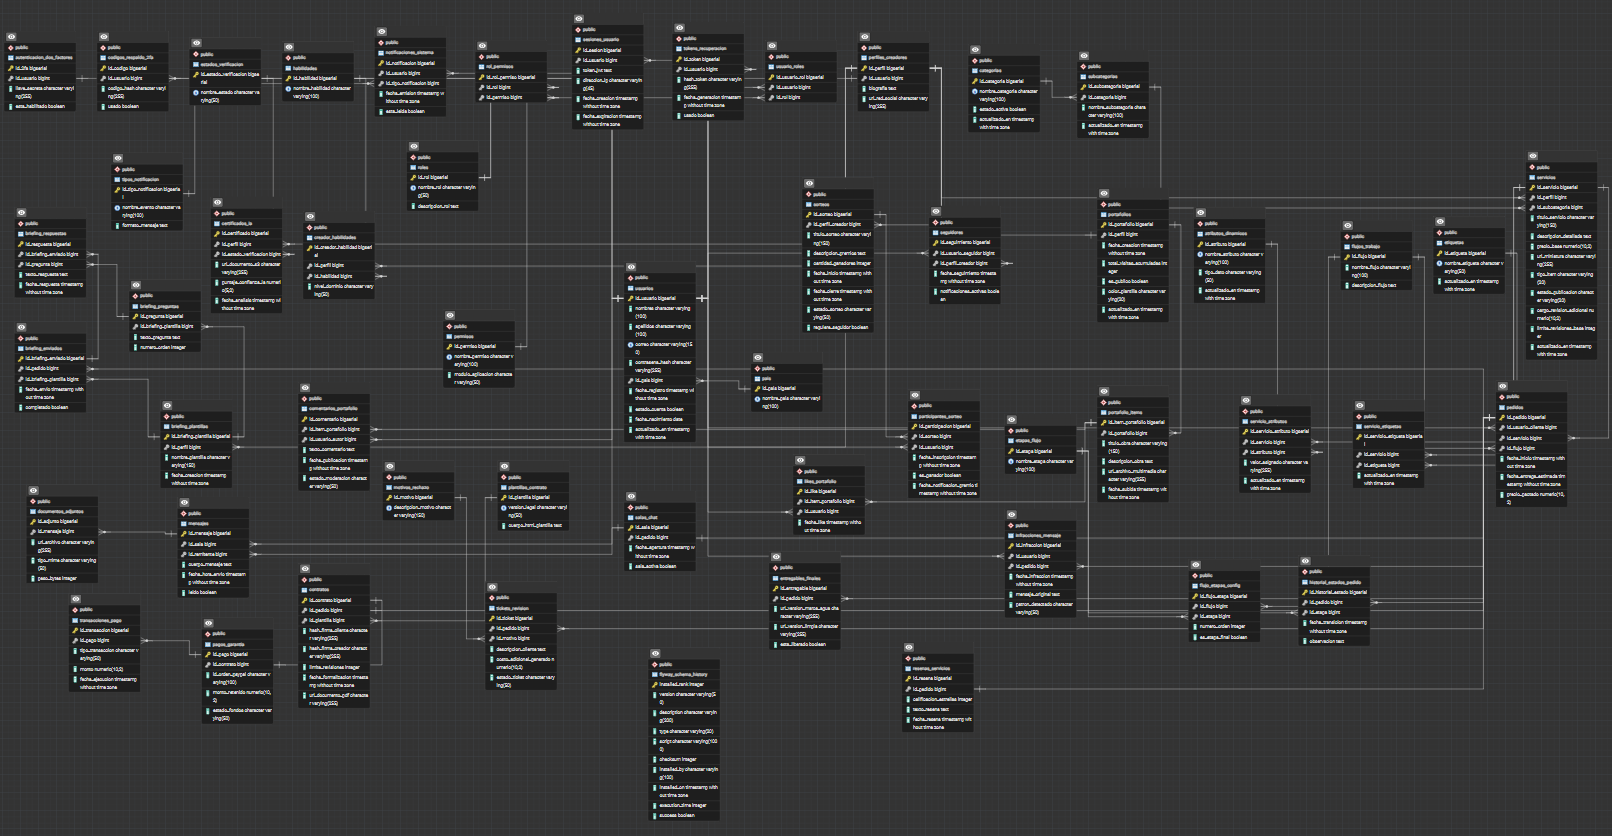
\includegraphics[width=6.26042in,height=3.39583in]{media/media/image4.png}

\begin{quote}
\textbf{6.1. Interfaz de catálogo inteligente y búsqueda (módulo de
cliente)}
\end{quote}

Esta pantalla constituye el punto de entrada principal para el
descubrimiento de servicios. Su diseño responsivo integra un panel
lateral de filtros combinados que permite segmentar la búsqueda por
categoría, rango de precio y etiquetas dinámicas. La grilla de
resultados expone las tarjetas de servicios priorizando la claridad
visual, mostrando únicamente la miniatura del producto, el precio base y
la calificación promedio del creador, optimizando la toma de decisiones
del cliente y cumpliendo con el motor de búsqueda especificado en los
requisitos del sistema.

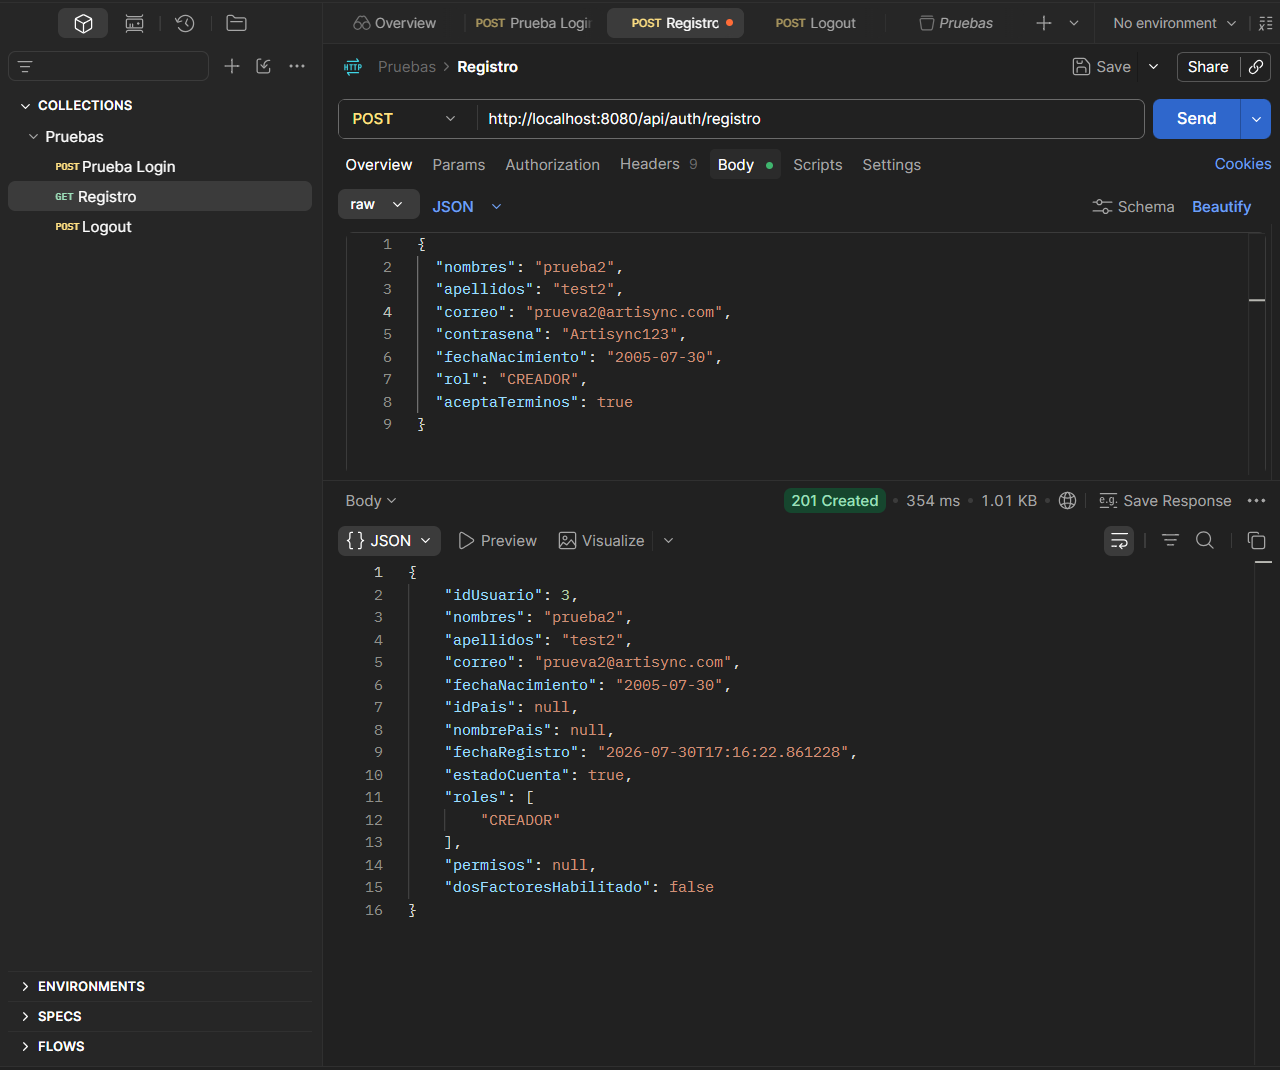
\includegraphics[width=6.26042in,height=3.35417in]{media/media/image5.png}

\begin{quote}
\textbf{6.2. Interfaz de perfil público del creador (módulo de identidad
y portafolio)} Diseñada para transmitir autoridad y confianza
profesional. La cabecera del perfil destaca los datos validados del
usuario, exhibiendo de forma prominente el "Sello de Verificación"
otorgado por el análisis de inteligencia artificial sobre los documentos
profesionales del creador. El cuerpo de la interfaz unifica la identidad
comercial, integrando métricas en tiempo real como el conteo de
seguidores y el promedio de calificaciones, además de organizar el
catálogo del creador en pestañas limpias que separan las obras previas
(Portafolio) de las comisiones activas (Servicios).
\end{quote}

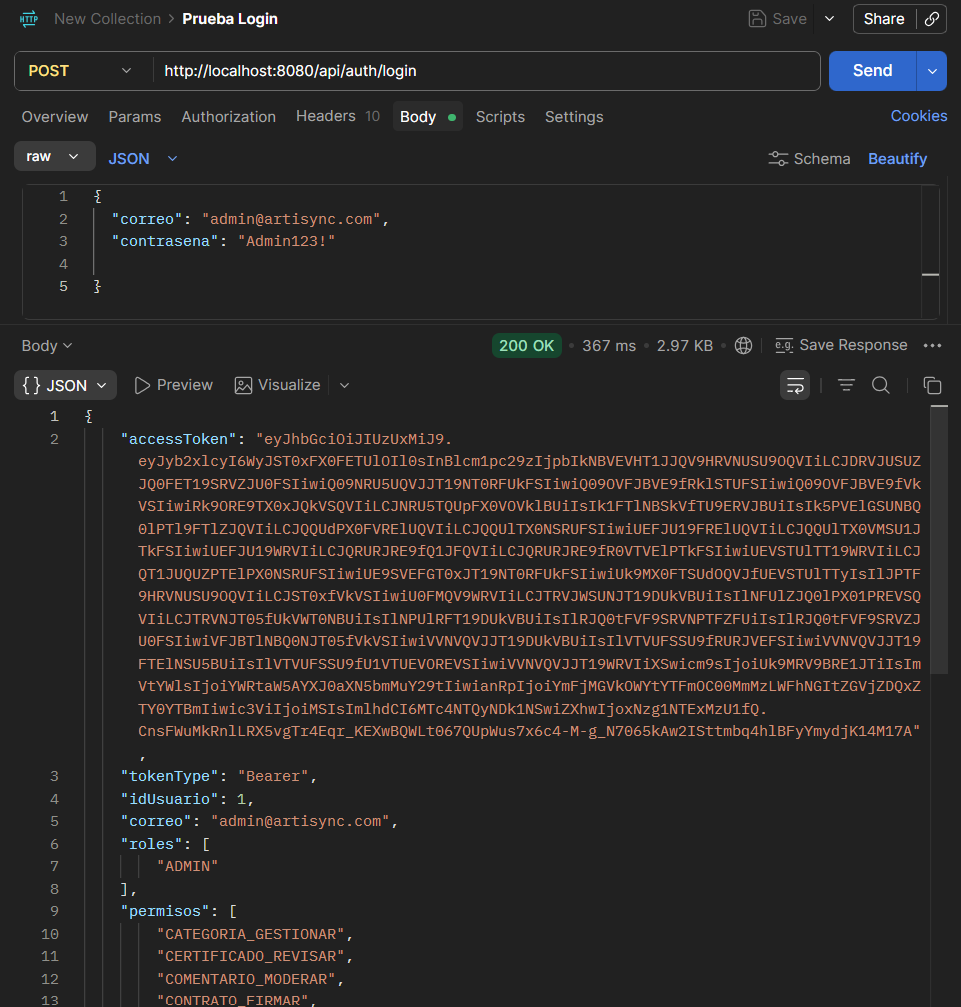
\includegraphics[width=6.26042in,height=2.86458in]{media/media/image6.png}

\begin{quote}
\textbf{6.3. Interfaz de sala de operaciones (módulo de comunicación y
legal)}
\end{quote}

Esta pantalla de diseño dividido (split-screen) centraliza la
negociación y formalización del servicio. El panel izquierdo aloja el
sistema de mensajería bidireccional en tiempo real (vía WebSockets), el
cual incluye el motor de validación en segundo plano para bloquear el
intercambio de datos de contacto externos. El panel derecho actúa como
un gestor de documentos dinámico, donde el formulario de briefing
interactivo se transforma automáticamente en un contrato digital
renderizado en HTML, habilitando las acciones de firma electrónica para
ambas partes y la posterior descarga en formato PDF.

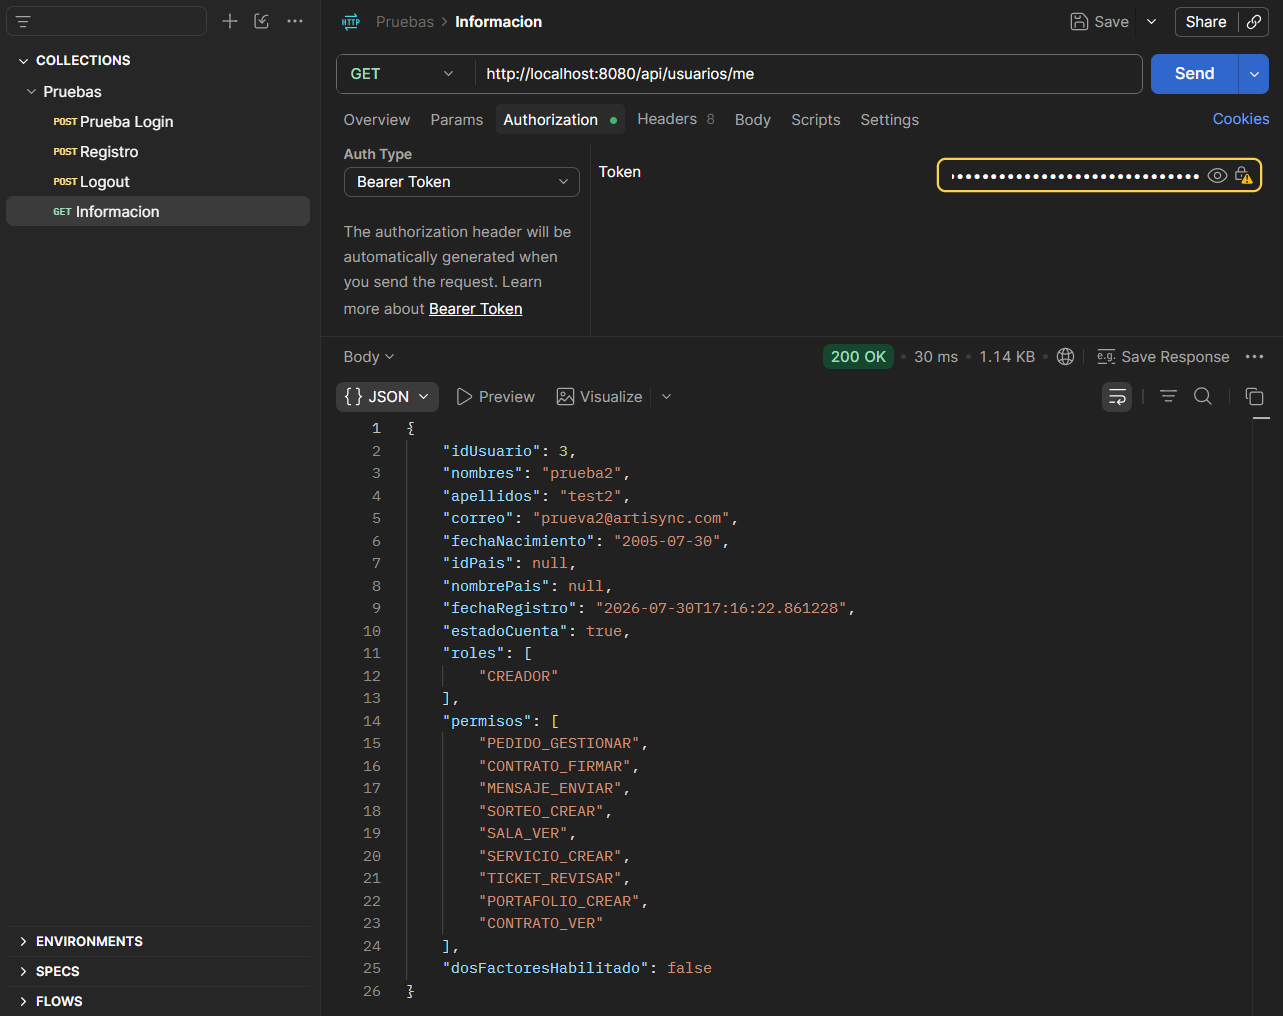
\includegraphics[width=6.26042in,height=3.42708in]{media/media/image7.png}

\begin{quote}
\textbf{6.4. Interfaz de pipeline de producción (módulo de flujos de
trabajo)}
\end{quote}

Orientada exclusivamente a la gestión operativa del creador, esta vista
adopta un tablero tipo Kanban para monitorear el ciclo de vida de los
pedidos activos. Las columnas representan las etapas configuradas en el
motor de flujos de trabajo (ej. \emph{En Espera, Boceto, Revisión,
Finalizado}). Al interactuar con las tarjetas de cada pedido, el creador
ejecuta las transiciones de estado que se registran automáticamente en
el historial de auditoría del sistema, permitiendo una trazabilidad
exacta y notificando al cliente sobre el avance de su comisión.

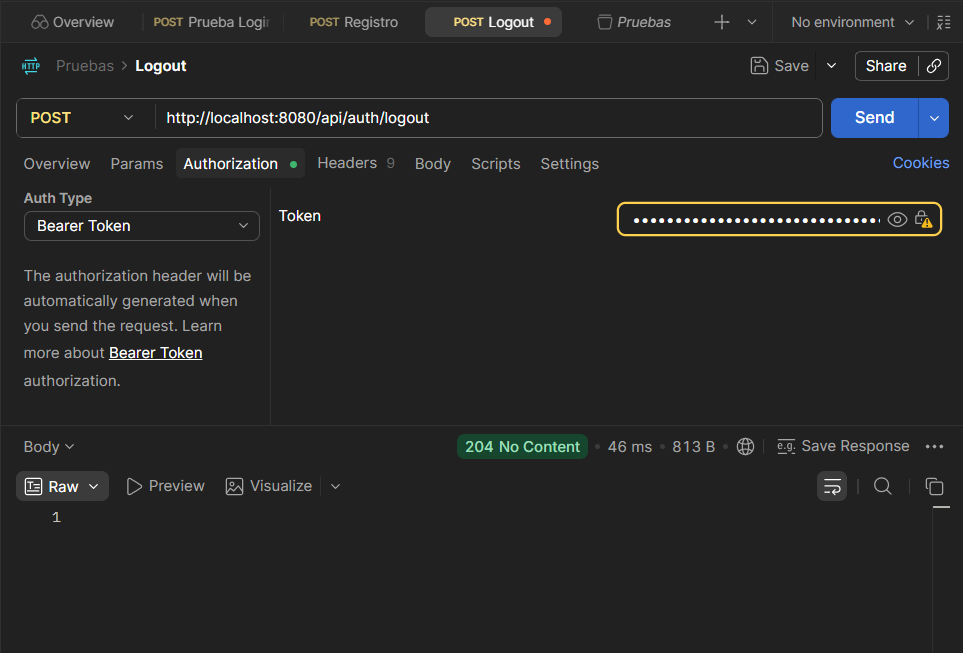
\includegraphics[width=6.26042in,height=3.25in]{media/media/image8.png}

\begin{quote}
\textbf{6.5. Interfaz de entrega final y escrow (módulo financiero y
entregables)}
\end{quote}

Esta pantalla representa la culminación técnica y financiera del ciclo
de servicio. Su estructura prioriza la previsualización segura del
entregable mediante la aplicación de una marca de agua automatizada. El
panel de acciones lateral cede el control final al cliente, ofreciendo
dos flujos condicionales: la solicitud de revisiones adicionales (con
recargo automatizado en caso de superar el límite del contrato) o la
aprobación definitiva del trabajo. La acción de aprobación desencadena
lógicamente la liberación de los fondos retenidos en la pasarela de pago
(Escrow) y habilita la descarga del archivo en su versión limpia y en
alta resolución.

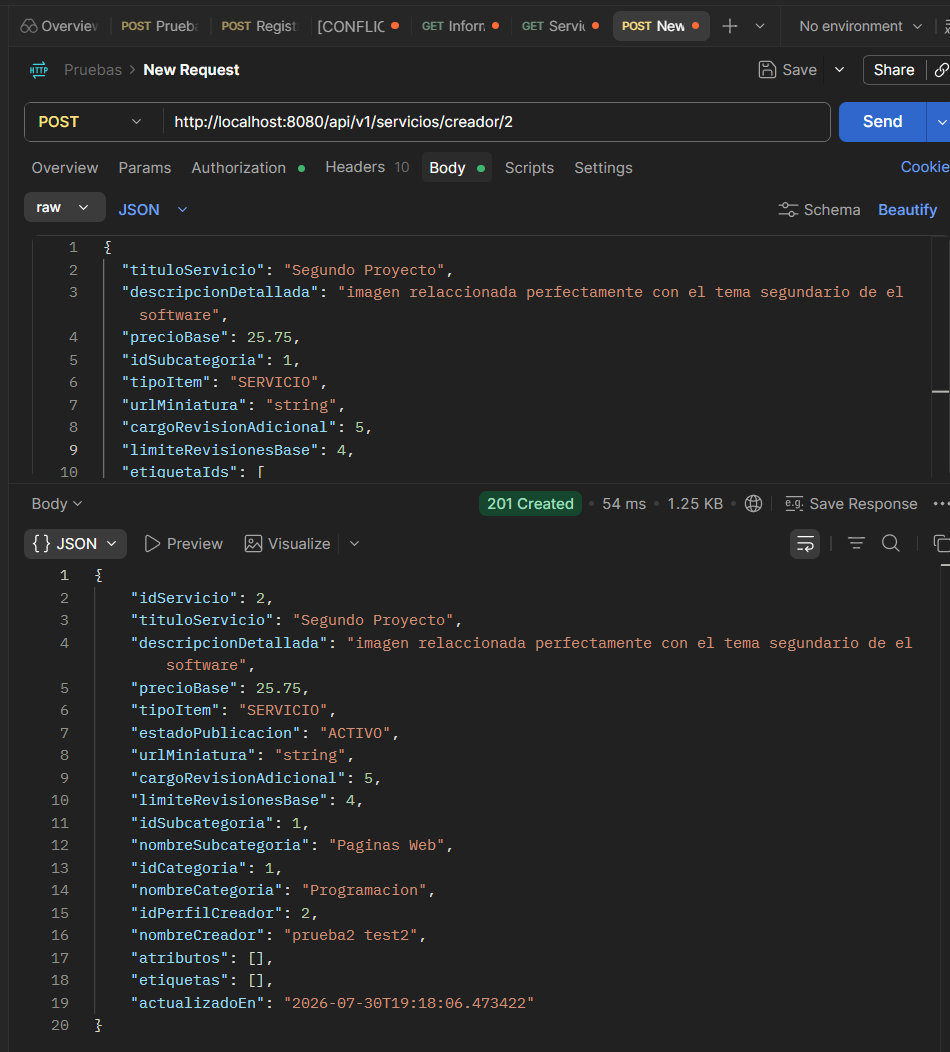
\includegraphics[width=6.26042in,height=3.36458in]{media/media/image9.png}

\textbf{7. Plan de trabajo: cronograma e hitos}

Esta sección documenta la planificación temporal del proyecto Artisync
desde la semana 5 hasta la semana 17 del período académico 2025-2026. El
equipo está conformado por tres integrantes: Johan C., Bryan F. y Jhon
R. El cronograma es coherente con las sumativas establecidas en el
sílabo. La asignación de responsable principal no limita el trabajo a un
solo módulo: el historial de commits en GitHub debe reflejar
contribuciones de los tres integrantes en todos los módulos del sistema.

\begin{quote}
\textbf{7.1. Cronograma en formato Gantt o tabla semanal}
\end{quote}

La siguiente tabla detalla para cada semana la tarea, la descripción
técnica vinculada a los módulos de la base de datos, el responsable
principal, su colaborador de apoyo, el entregable del sílabo y la
sumativa correspondiente:

\begin{longtable}[]{@{}
  >{\raggedright\arraybackslash}p{(\columnwidth - 10\tabcolsep) * \real{0.0780}}
  >{\raggedright\arraybackslash}p{(\columnwidth - 10\tabcolsep) * \real{0.3411}}
  >{\raggedright\arraybackslash}p{(\columnwidth - 10\tabcolsep) * \real{0.1764}}
  >{\raggedright\arraybackslash}p{(\columnwidth - 10\tabcolsep) * \real{0.1827}}
  >{\raggedright\arraybackslash}p{(\columnwidth - 10\tabcolsep) * \real{0.0813}}
  >{\raggedright\arraybackslash}p{(\columnwidth - 10\tabcolsep) * \real{0.1406}}@{}}
\toprule\noalign{}
\begin{minipage}[b]{\linewidth}\raggedright
\textbf{Sem.}
\end{minipage} & \begin{minipage}[b]{\linewidth}\raggedright
\textbf{Tarea principal y detalle técnico}
\end{minipage} & \begin{minipage}[b]{\linewidth}\raggedright
\textbf{Responsable}
\end{minipage} & \begin{minipage}[b]{\linewidth}\raggedright
\textbf{Entregable}
\end{minipage} & \begin{minipage}[b]{\linewidth}\raggedright
\textbf{Sum.}
\end{minipage} & \begin{minipage}[b]{\linewidth}\raggedright
\textbf{Tipo}
\end{minipage} \\
\midrule\noalign{}
\endhead
\bottomrule\noalign{}
\endlastfoot
\textbf{S5} & \textbf{Entrega 1A: diseño y planificación}

ER conceptual/lógico/físico, C4 Nivel 1 y 2, ADR-001, cronograma,
asignación de roles. & \textbf{Todo el equipo} & PDF Entrega 1A en LMS &
\textbf{S\#5} & \textbf{Entrega} \\
\textbf{S6} & Configuración del entorno + estructura del proyecto +
primeras rutas

Repositorio GitHub, estructura Spring Boot + Angular 17, Dockerfiles,
ruta /api/health, Angular routing inicial. &
\begin{minipage}[t]{\linewidth}\raggedright
\textbf{Johan C.}\\
Apoyo: Bryan F.\strut
\end{minipage} & Repositorio con estructura inicial & --- &
\textbf{Trabajo} \\
\textbf{S7} & PE Unidad II: backend con Java/Spring Boot

Johan: ORM base. Bryan: servicios. Jhon: pruebas. Commits de los tres
integrantes obligatorios. & \textbf{Todo el equipo} & Práctica
Experimental U2 & \textbf{S\#6} & \textbf{Sumativa} \\
\textbf{S8} & Tutoría --- consolidar avances y resolver blockers

Revisión de progreso, pull requests revisados, resolución de problemas
de integración entre capas. & \textbf{Todo el equipo} & --- & --- &
\textbf{Tutoría} \\
\textbf{S9} & Evaluación Parcial 1 (individual)

Evaluación individual. Semana de repaso, sin push de features nuevas al
repositorio. & \begin{minipage}[t]{\linewidth}\raggedright
\textbf{Todo el equipo}\\
Individual\strut
\end{minipage} & EP Primer Corte & \textbf{S\#7} &
\textbf{Evaluación} \\
\textbf{S10} & Módulo de autenticación completo + sesiones (Spring
Security, JWT, 2FA)

Tablas: usuarios, roles, permisos, sesiones\_usuario,
autenticacion\_dos\_factores, tokens\_recuperacion. &
\begin{minipage}[t]{\linewidth}\raggedright
\textbf{Johan C.}\\
Apoyo: Jhon R.\strut
\end{minipage} & Avance PFC --- Módulo datos & \textbf{S\#8} &
\textbf{Sumativa} \\
\textbf{S11} & CRUD entidad principal + ORM (servicios, pedidos,
categorías)

Entidades JPA: servicios, categorias, subcategorias, pedidos,
historial\_estados\_pedido. Bean Validation. &
\begin{minipage}[t]{\linewidth}\raggedright
\textbf{Bryan F.}\\
Apoyo: Johan C.\strut
\end{minipage} & PE Unidad III & \textbf{S\#9} & \textbf{Sumativa} \\
\textbf{S12} & Integración de capas + Escrow + chat (Módulos M5/M6)

Módulos: pagos\_garantia, contratos, salas\_chat, mensajes,
notificaciones. Pruebas JUnit 5 + MockMvc. &
\begin{minipage}[t]{\linewidth}\raggedright
\textbf{Jhon R.}\\
Apoyo: Bryan F.\strut
\end{minipage} & --- & --- & \textbf{Trabajo} \\
\textbf{S13} & Frontend responsivo + segunda entidad (Angular +
Bootstrap 5)

Módulo Angular: portafolio-items, catálogo EAV, formulario de pedido,
guards de ruta con JWT. & \begin{minipage}[t]{\linewidth}\raggedright
\textbf{Johan C.}\\
Apoyo: Jhon R.\strut
\end{minipage} & Exposición Back-End & \textbf{S\#12} &
\textbf{Sumativa} \\
\textbf{S14} & Implementación MVC completa + API REST (integración total
backend-frontend)

Integrar los 7 módulos de la BD. Sorteos, notificaciones, seguidores.
API REST documentada con Swagger. & \textbf{Todo el equipo} & --- & ---
& \textbf{Trabajo} \\
\textbf{S15} & \textbf{Entrega 1B: implementación + documentación
completa}

Documentación técnica, manual de usuario, video demo, código en GitHub,
PDF Entrega 1B. & \textbf{Todo el equipo} & Entrega 1B en LMS &
\textbf{S\#15} & \textbf{Entrega} \\
\textbf{S16} & PE Unidad IV + pruebas de aceptación

Práctica Experimental IV. Pruebas de aceptación con datos reales.
Corrección de bugs críticos. & \textbf{Todo el equipo} & PE Unidad IV &
\textbf{S\#16} & \textbf{Sumativa} \\
\textbf{S17} & \textbf{Defensa oral del PFC}

Presentación final del sistema. Demo en vivo. Cada integrante expone su
módulo asignado. & \textbf{Todo el equipo} & EP Segundo Corte + defensa
& \textbf{S\#17} & \textbf{Defensa} \\
\end{longtable}

\textbf{7.2. Asignación de roles del equipo}

\begin{longtable}[]{@{}
  >{\raggedright\arraybackslash}p{(\columnwidth - 8\tabcolsep) * \real{0.1725}}
  >{\raggedright\arraybackslash}p{(\columnwidth - 8\tabcolsep) * \real{0.1766}}
  >{\raggedright\arraybackslash}p{(\columnwidth - 8\tabcolsep) * \real{0.2984}}
  >{\raggedright\arraybackslash}p{(\columnwidth - 8\tabcolsep) * \real{0.1528}}
  >{\raggedright\arraybackslash}p{(\columnwidth - 8\tabcolsep) * \real{0.1998}}@{}}
\toprule\noalign{}
\begin{minipage}[b]{\linewidth}\raggedright
\textbf{Integrante}
\end{minipage} & \begin{minipage}[b]{\linewidth}\raggedright
\textbf{Rol principal}
\end{minipage} & \begin{minipage}[b]{\linewidth}\raggedright
\textbf{Módulos BD asignados}
\end{minipage} & \begin{minipage}[b]{\linewidth}\raggedright
\textbf{Sem. responsable}
\end{minipage} & \begin{minipage}[b]{\linewidth}\raggedright
\textbf{Política de commits}
\end{minipage} \\
\midrule\noalign{}
\endhead
\bottomrule\noalign{}
\endlastfoot
\textbf{Johan C.} & \textbf{Líder técnico / Full-Stack} & M1 Seguridad
(S10): usuarios, roles, JWT, 2FA, sesiones. M3 Catálogo EAV (S13):
servicios, atributos, etiquetas. Frontend Angular (S13): routing,
guards, módulo catálogo. & S6, S10, S13 & \emph{Min. 2 commits/semana.
Code review de M5 en S12.} \\
\textbf{Bryan F.} & \textbf{Desarrollador Backend / Datos} & M4 Pedidos
y Flujos (S11): pedidos, flujos\_trabajo, etapas\_flujo,
historial\_estados, tickets\_revision. CRUD JPA/Hibernate. Pruebas
unitarias JUnit 5. & S11, S12 (apoyo) & \emph{Min. 2 commits/semana.
Code review de M7 en S14.} \\
\textbf{Jhon R.} & \textbf{Desarrollador Backend / Integración} & M5
Legal y Escrow (S12): contratos, pagos\_garantia, entregables\_finales,
transacciones\_pago. M6 Comunicación (S12): salas\_chat, mensajes,
notificaciones. Pruebas de integración. & S12, S13 (apoyo) & \emph{Min.
2 commits/semana. Code review de M2 en S10.} \\
\end{longtable}

\textbf{8. Estructura del repositorio Git}

├── .github/

│ └── workflows/ \# Opcional (para integración continua futura)

├── database/

│ └── schema.sql \# Script DDL completo y ejecutable de PostgreSQL
{[}cite: 744, 794

├── docs/

│ ├── adr/

│ │ └── ADR-001-tecnologia.md \# Registro de decisión arquitectónica
(Java/Spring Boot)

│ ├── diagramas/

│ │ ├── c4-nivel1-contexto.png

│ │ ├── c4-nivel2-contenedores.png

│ │ ├── mer-base-datos.png \# Diagrama Entidad-Relación

│ │ └── wireframes/ \# Capturas o exportaciones de las 4+ interfaces

│ └── entrega-1a.pdf \# El informe final en formato PDF

├── .env.example \# Variables de entorno de muestra (sin credenciales
reales)

├── .gitignore \# Filtro para ignorar node\_modules, .env, target/, etc.

└── README.md \# Descripción del proyecto, integrantes e instrucciones

\textbf{9. Referencias bibliográficas}

{[}1{]} S. Coello Quezada, O. Peñafiel Chele, and Á. Yanza Montalván,
``Desarrollo de una aplicación web e-commerce B2C mediante tecnologías
de desarrollo front-end y back-end. Caso de estudio ferretería `El
Descanso,'\,'' \emph{Investigación, Tecnología e Innovación}, vol. 15,
no. 19, Jul. 2023, doi: 10.53591/ITI.V15I19.1525.

{[}2{]} R. Peres, M. Schreier, D. A. Schweidel, and A. Sorescu, ``The
creator economy: An introduction and a call for scholarly research,''
\emph{International Journal of Research in Marketing}, vol. 41, no. 3,
pp. 403--410, Sep. 2024, doi: 10.1016/j.ijresmar.2024.07.005.

{[}3{]} L. Gussek, A. Grabbe, and M. Wiesche, ``Challenges of IT
freelancers on digital labor platforms: A topic model approach,''
\emph{Electronic Markets 2023 33:1}, vol. 33, no. 1, pp. 55-, Oct. 2023,
doi: 10.1007/S12525-023-00675-Y.

{[}4{]} W. Tafesse and M. Dayan, ``Content creators' participation in
the creator economy: Examining the effect of creators' content sharing
frequency on user engagement behavior on digital platforms,''
\emph{Journal of Retailing and Consumer Services}, vol. 73, Jul. 2023,
doi: 10.1016/J.JRETCONSER.2023.103357.

{[}5{]} P. Monsalve-Obreque, P. Vargas-Villarroel, Y.
Hormazabal-Astorga, J. Hochstetter-Diez, J. Bustos-Gómez, and M.
Diéguez-Rebolledo, ``Proposal to Improve the E-Commerce Platform
Development Process with an Exploratory Case Study in Chile,''
\emph{Applied Sciences (Switzerland)}, vol. 13, no. 14, Jul. 2023, doi:
10.3390/APP13148362.

{[}6{]} T. Wulfert and R. Schütte, ``Retailer's Dual Role in Digital
Marketplaces,'' \emph{SN Computer Science 2022 3:3}, vol. 3, no. 3, pp.
206-, Mar. 2022, doi: 10.1007/S42979-022-01098-W.

\end{document}
